\section{Platform Components}

\subsection{AutoML}
Given a dataset to AutoML, it streamlines the process of finding the best model.\\

AutoML experiments with different \textit{features, algorithmes and hyperparameters}. The model can then by exported into \gls{g_ONNX} to be used on various platforms and devices. 

\begin{figure}[H]
	\centering
	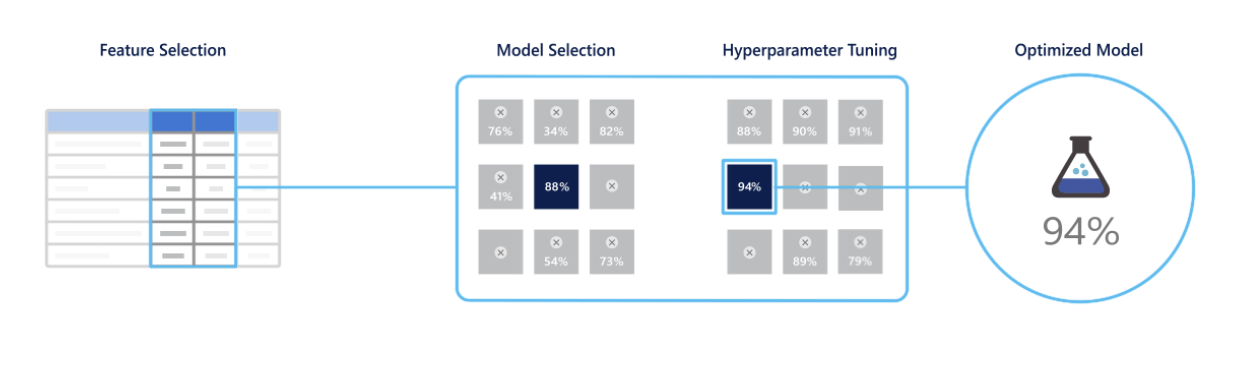
\includegraphics[scale = 0.4]{attachment/chapter_10/Scc004}
	\caption{AutoML Process}
\end{figure}

In the first step, for different Models different features will be tested. If the models scores well, then the hyperparametesation takes place. All the parameter, which goes into building the model will be tuned.

\subsection{Datasets}
The component \textit{Datasets} can be thought of as Linked Cloud Data sources and build-in data store.

\subsubsection{Linked Cloud Data Sources}

Because it is a Azure service many azure services can be linked to it. For example
\begin{itemize}
	\item Azure Data Lake
	\item Azure Blob Storage
	\item SQL Database
	\item Databricks File System
\end{itemize}

\begin{figure}[H]
	\centering
	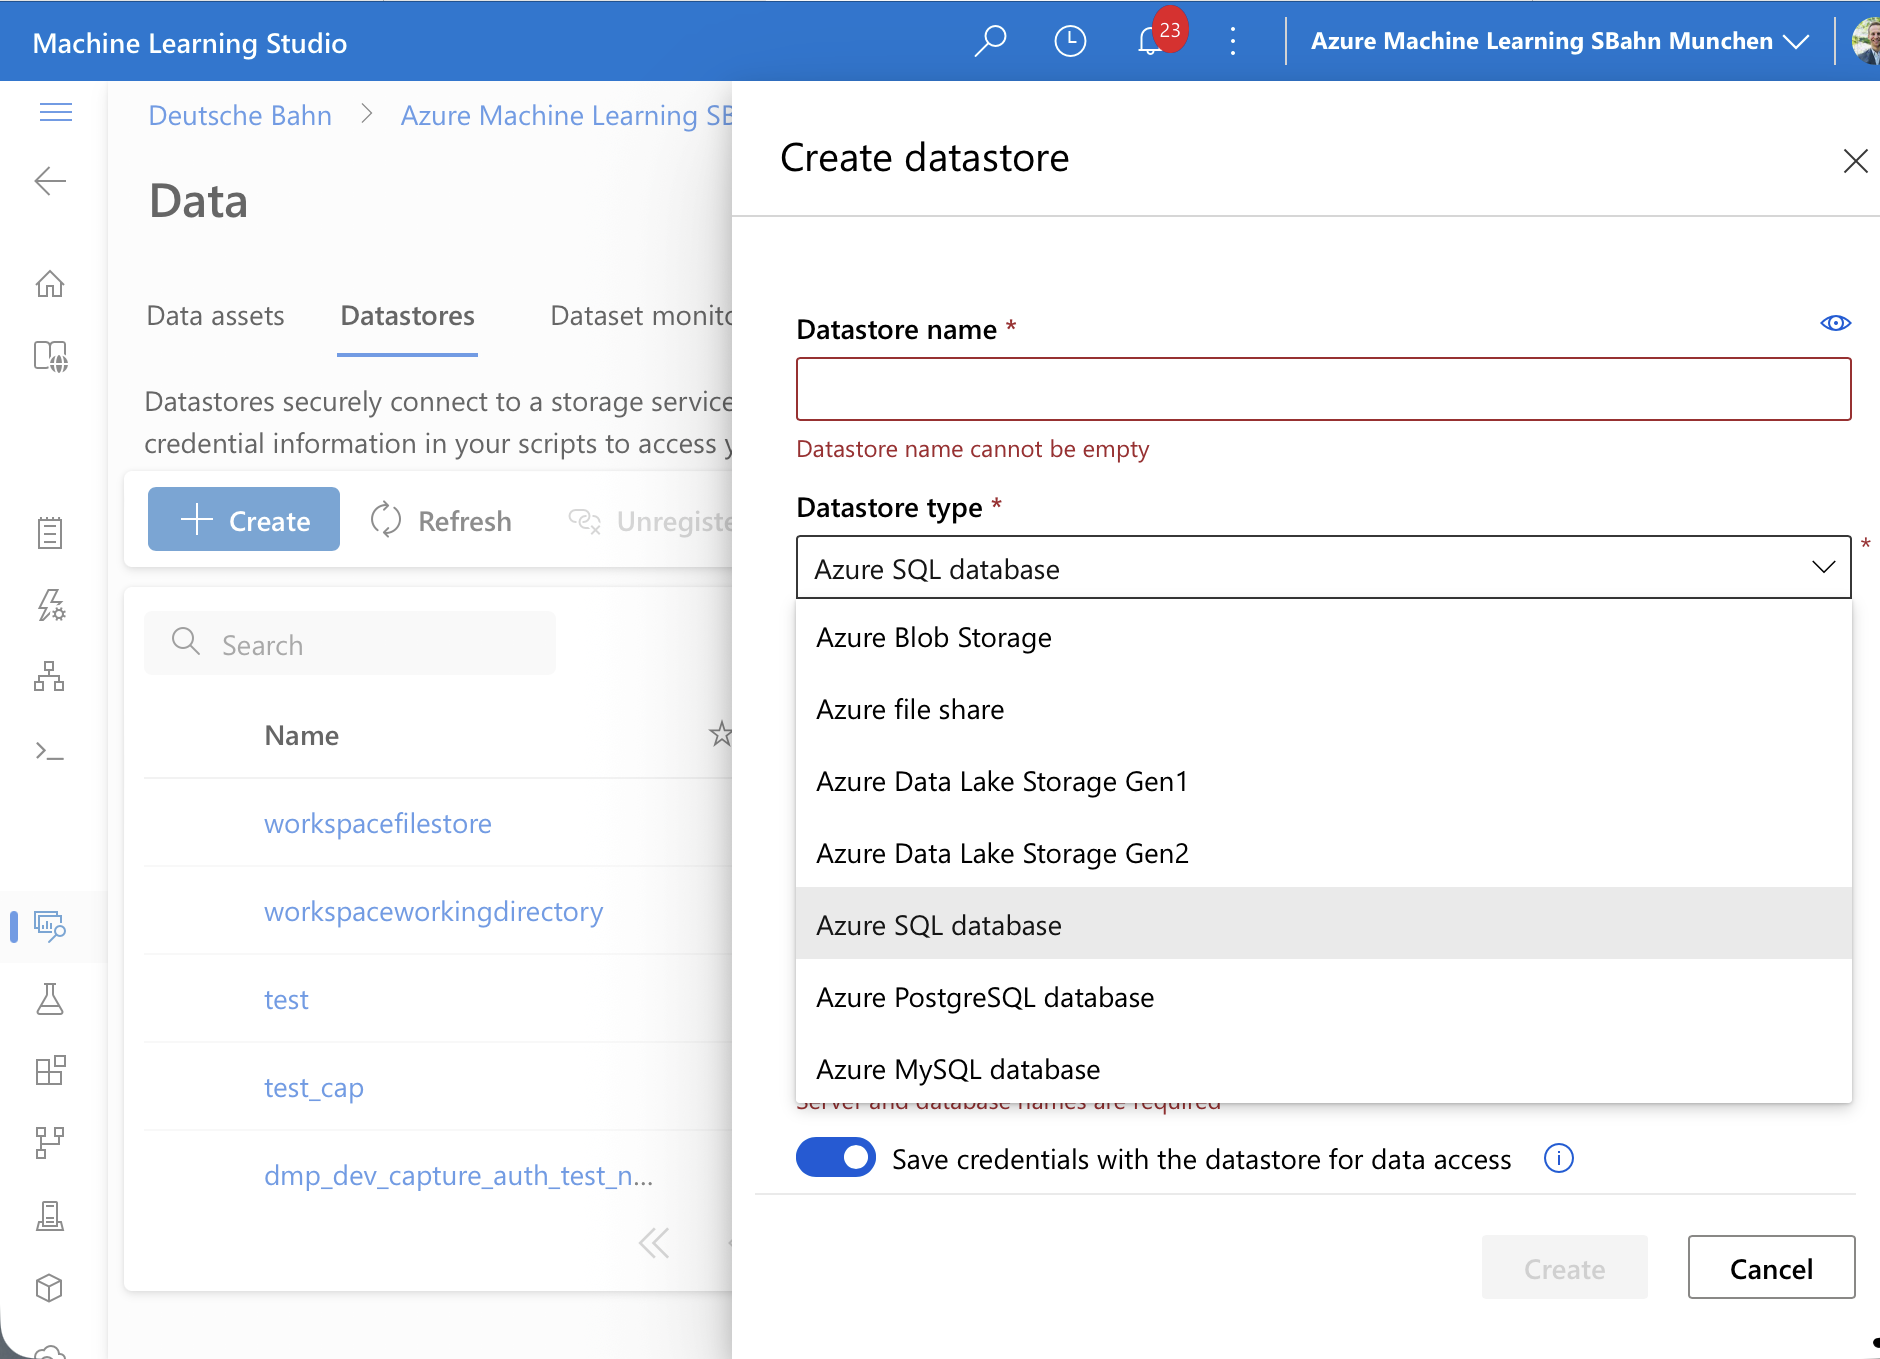
\includegraphics[scale = 0.2]{attachment/chapter_10/Scc028}
	\caption{Create a data storage connection}
\end{figure}

To note: Currently a link to a dedicated \gls{SQL} pool is not available. From those connection datasets are created.\\

A dataset can den be created from previous conneced datastore or from a local file or example registered datasets provided by \textit{Azure}.

\begin{figure}[H]
	\centering
	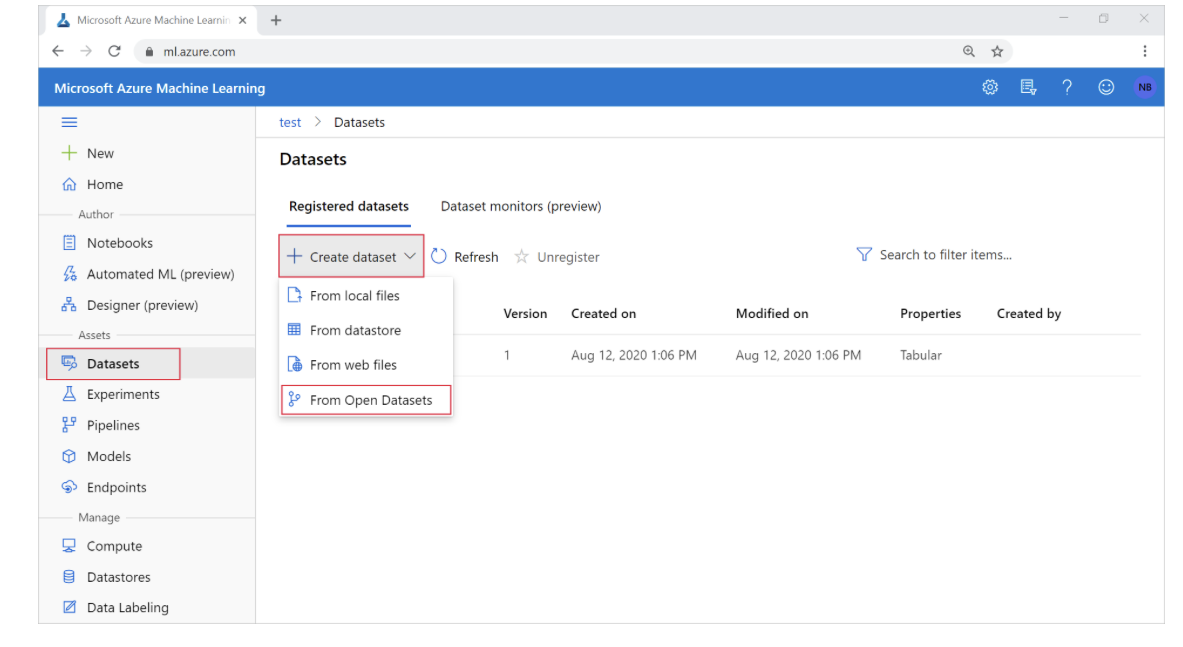
\includegraphics[scale = 0.2]{attachment/chapter_10/Scc006}\\ 
		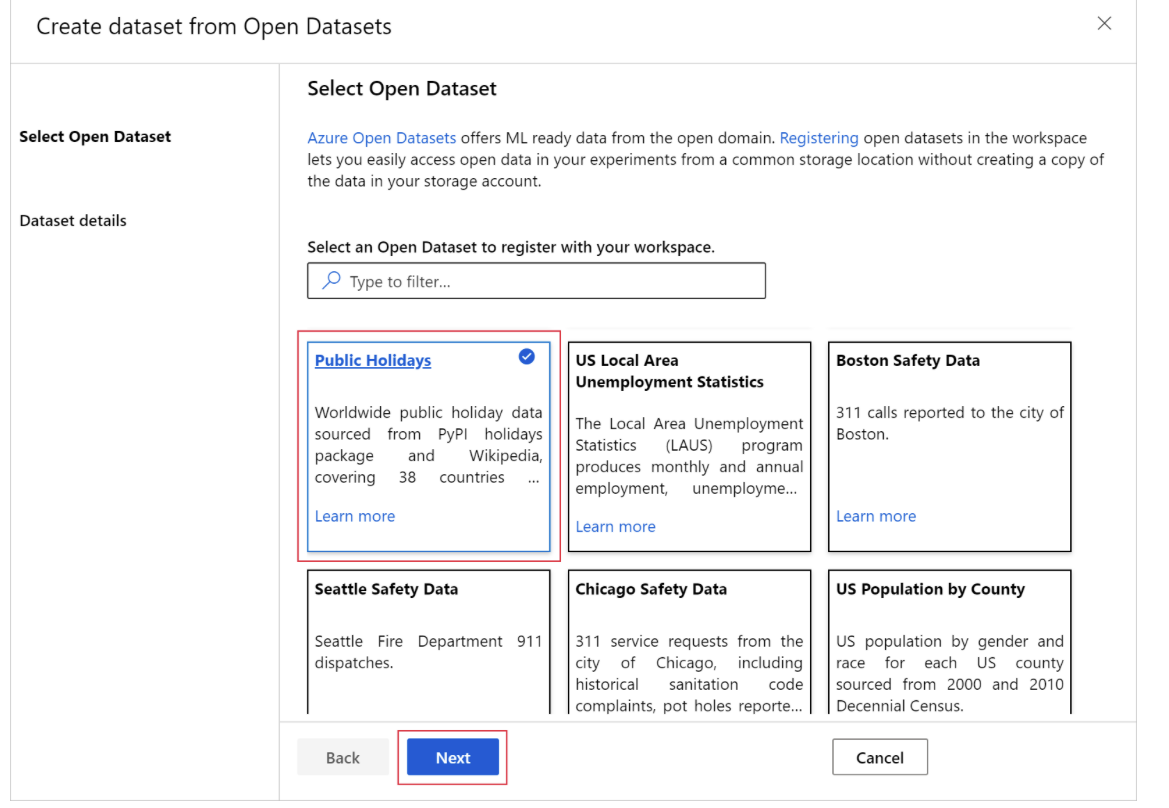
\includegraphics[scale = 0.2]{attachment/chapter_10/Scc007}
	\caption{Create a dataset}
\end{figure}

There are a variety of suppored data type 

\begin{figure}[H]
	\centering
	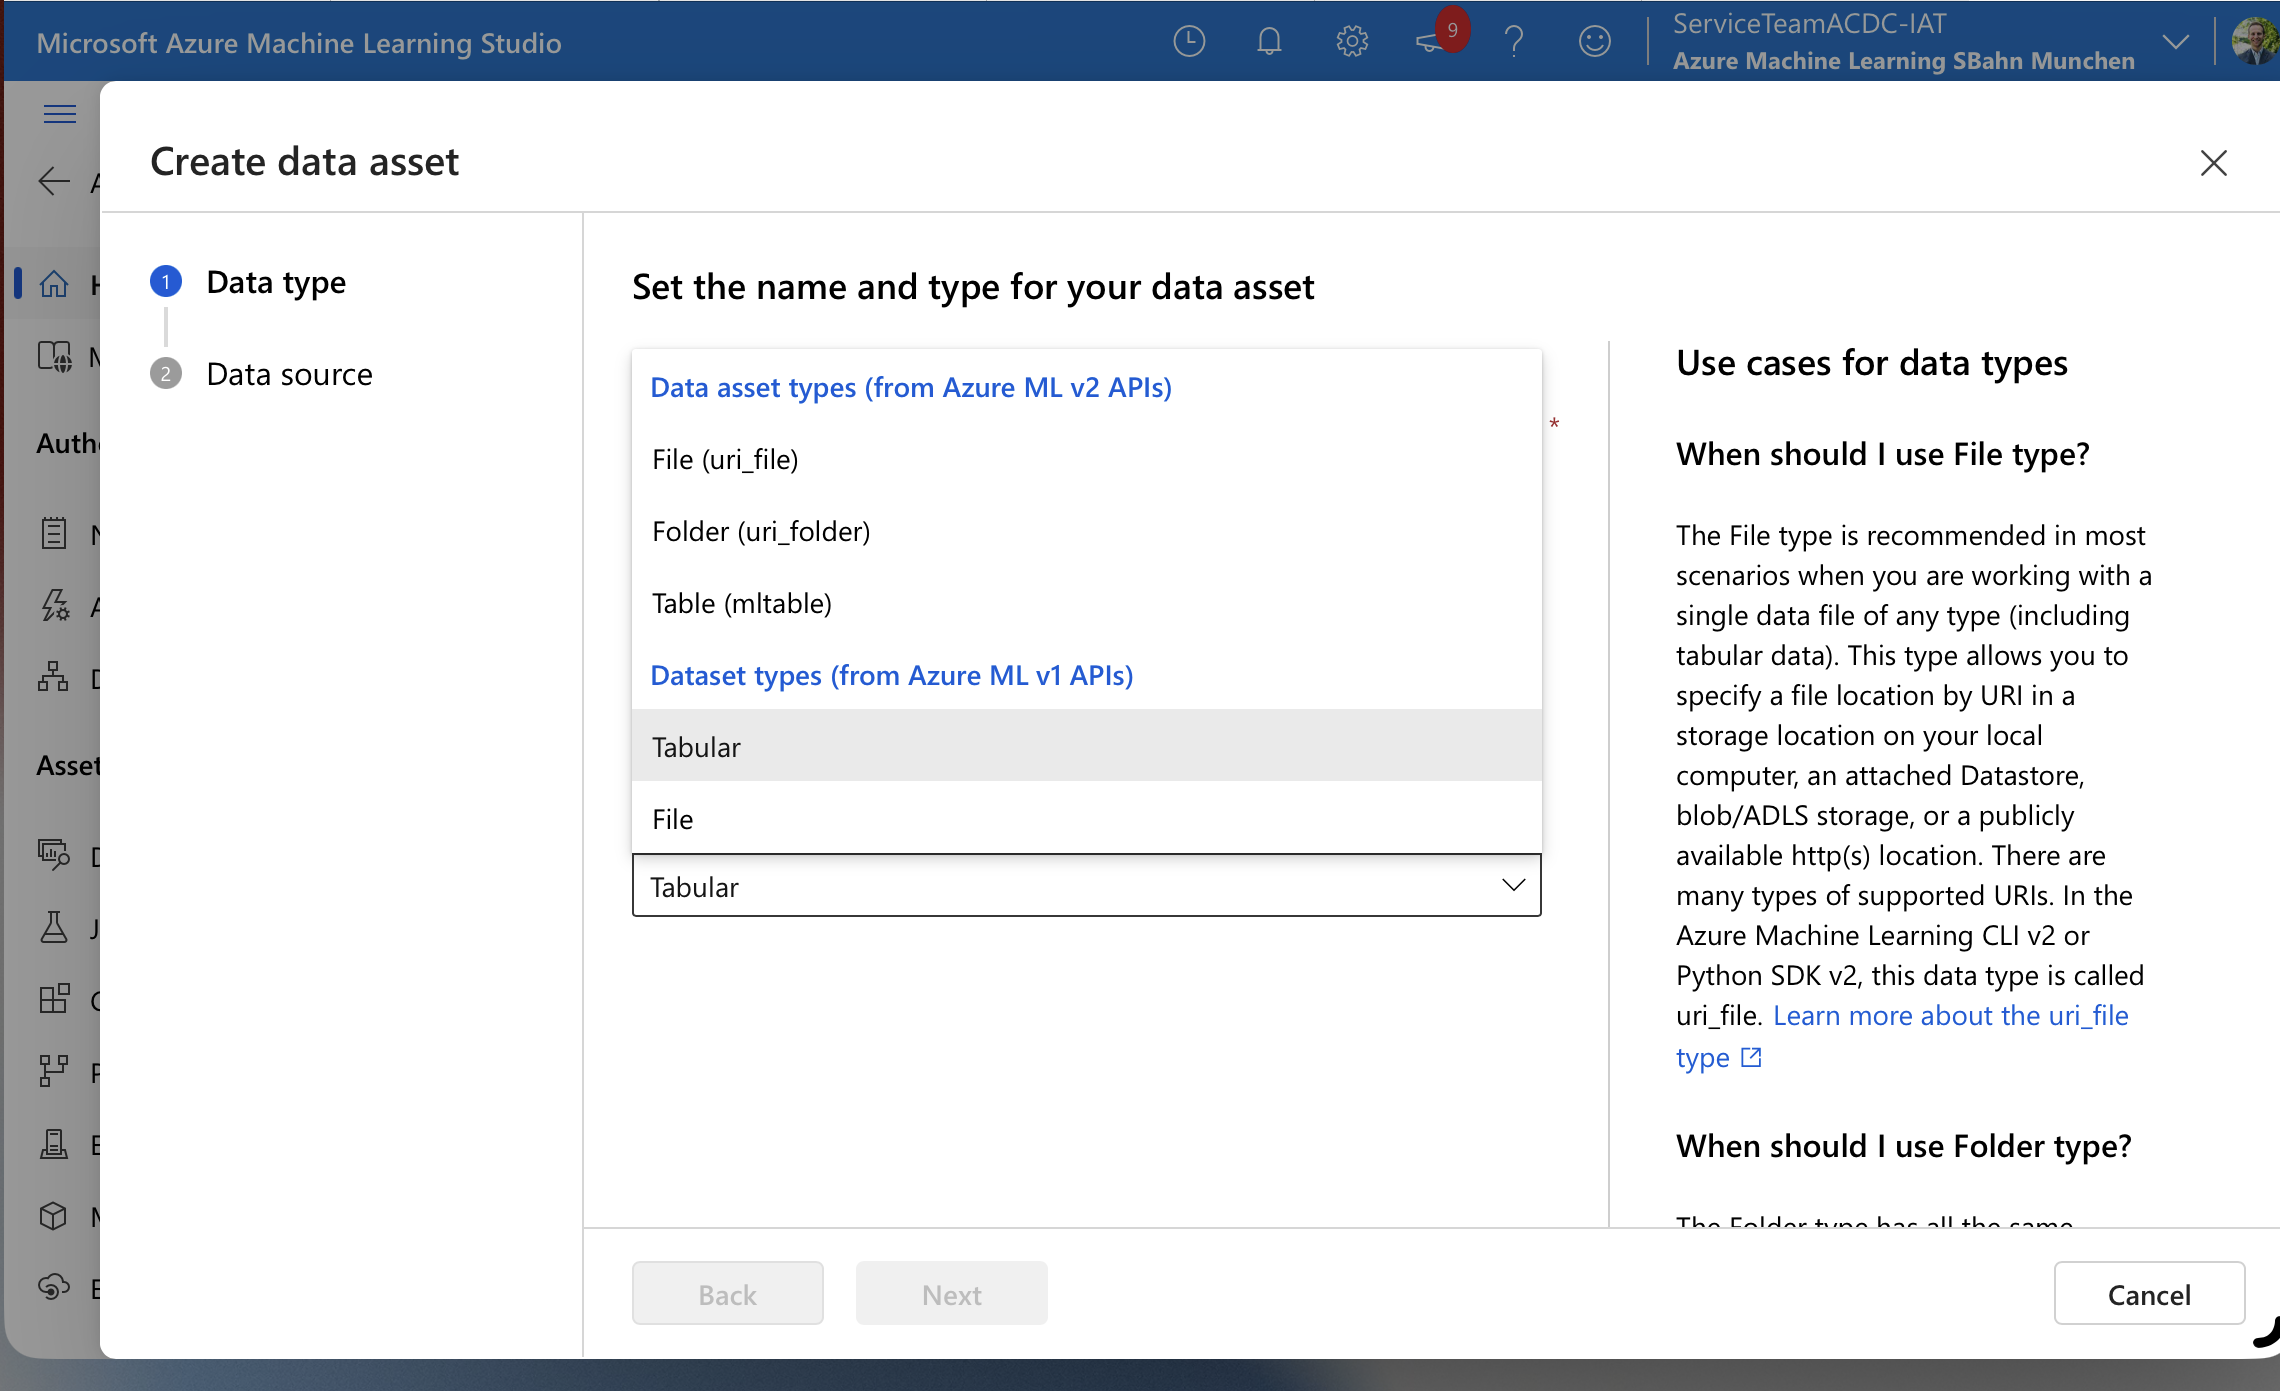
\includegraphics[scale = 0.1]{attachment/chapter_10/Scc008}
	\caption{New dataset types}
\end{figure}

A dataset can be 
\begin{itemize}
	\item registers, to allow others to work with it 
	\item versioned, to see the changes in the schema or data inside
\end{itemize}

In summery the dataset is a pointer to the datastore, where the data lifs.

\subsubsection{Build-in Data Store: Three Systems}
When you create a workspace, an Azure blob container and an Azure file share are automatically registered as datastores to the workspace.They're named \textit{workspaceblobstore} and \textit{workspacefilestore}, respectively. The workspaceblobstore is used to store \textbf{workspace artifacts} and your machine learning \textbf{experiment logs}. It's also set as the default datastore and can't be deleted from the workspace. The workspacefilestore is used to store \textbf{notebooks} and \textbf{R scripts} \underline{authorized via compute instance}.

\begin{lstlisting}[style=python]
import azureml.core
from azureml.core import Workspace, Datastore
     
ws = Workspace.from_config()	
\end{lstlisting}

\begin{figure}[H]
	\centering
	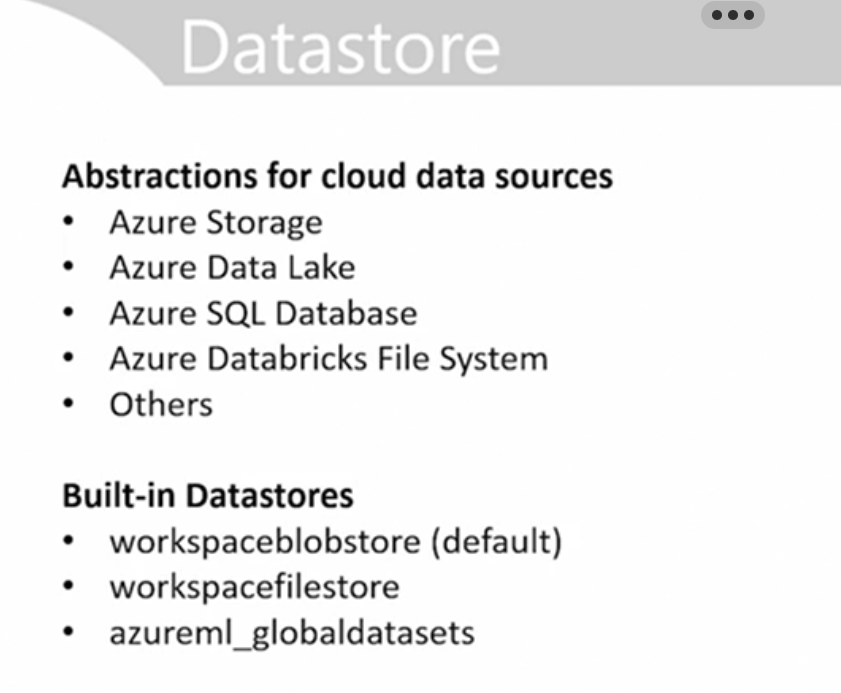
\includegraphics[scale = 0.3]{attachment/chapter_10/Scc029}
	\caption{Type of datasets}
\end{figure}

[!NOTE] Azure Machine Learning designer will create a datastore named \textit{azureml globaldatasets} automatically when you open a sample in the designer homepage. This datastore \textbf{only contains sample datasets} . Please do not use this datastore for any confidential data access.

\subsubsection{Example: Filestore}
In summery: Three workspace resources are created

	\begin{description}
		\centering
		\item[blobstore (default)] Artifacts of \gls{ML} Expermiments logs
		\item[filestore] Notebooks, Scripts
		\item[azureml globaldatasets]
	\end{description}

In the workspace this are further separated.

\begin{figure}[H]
	\centering
	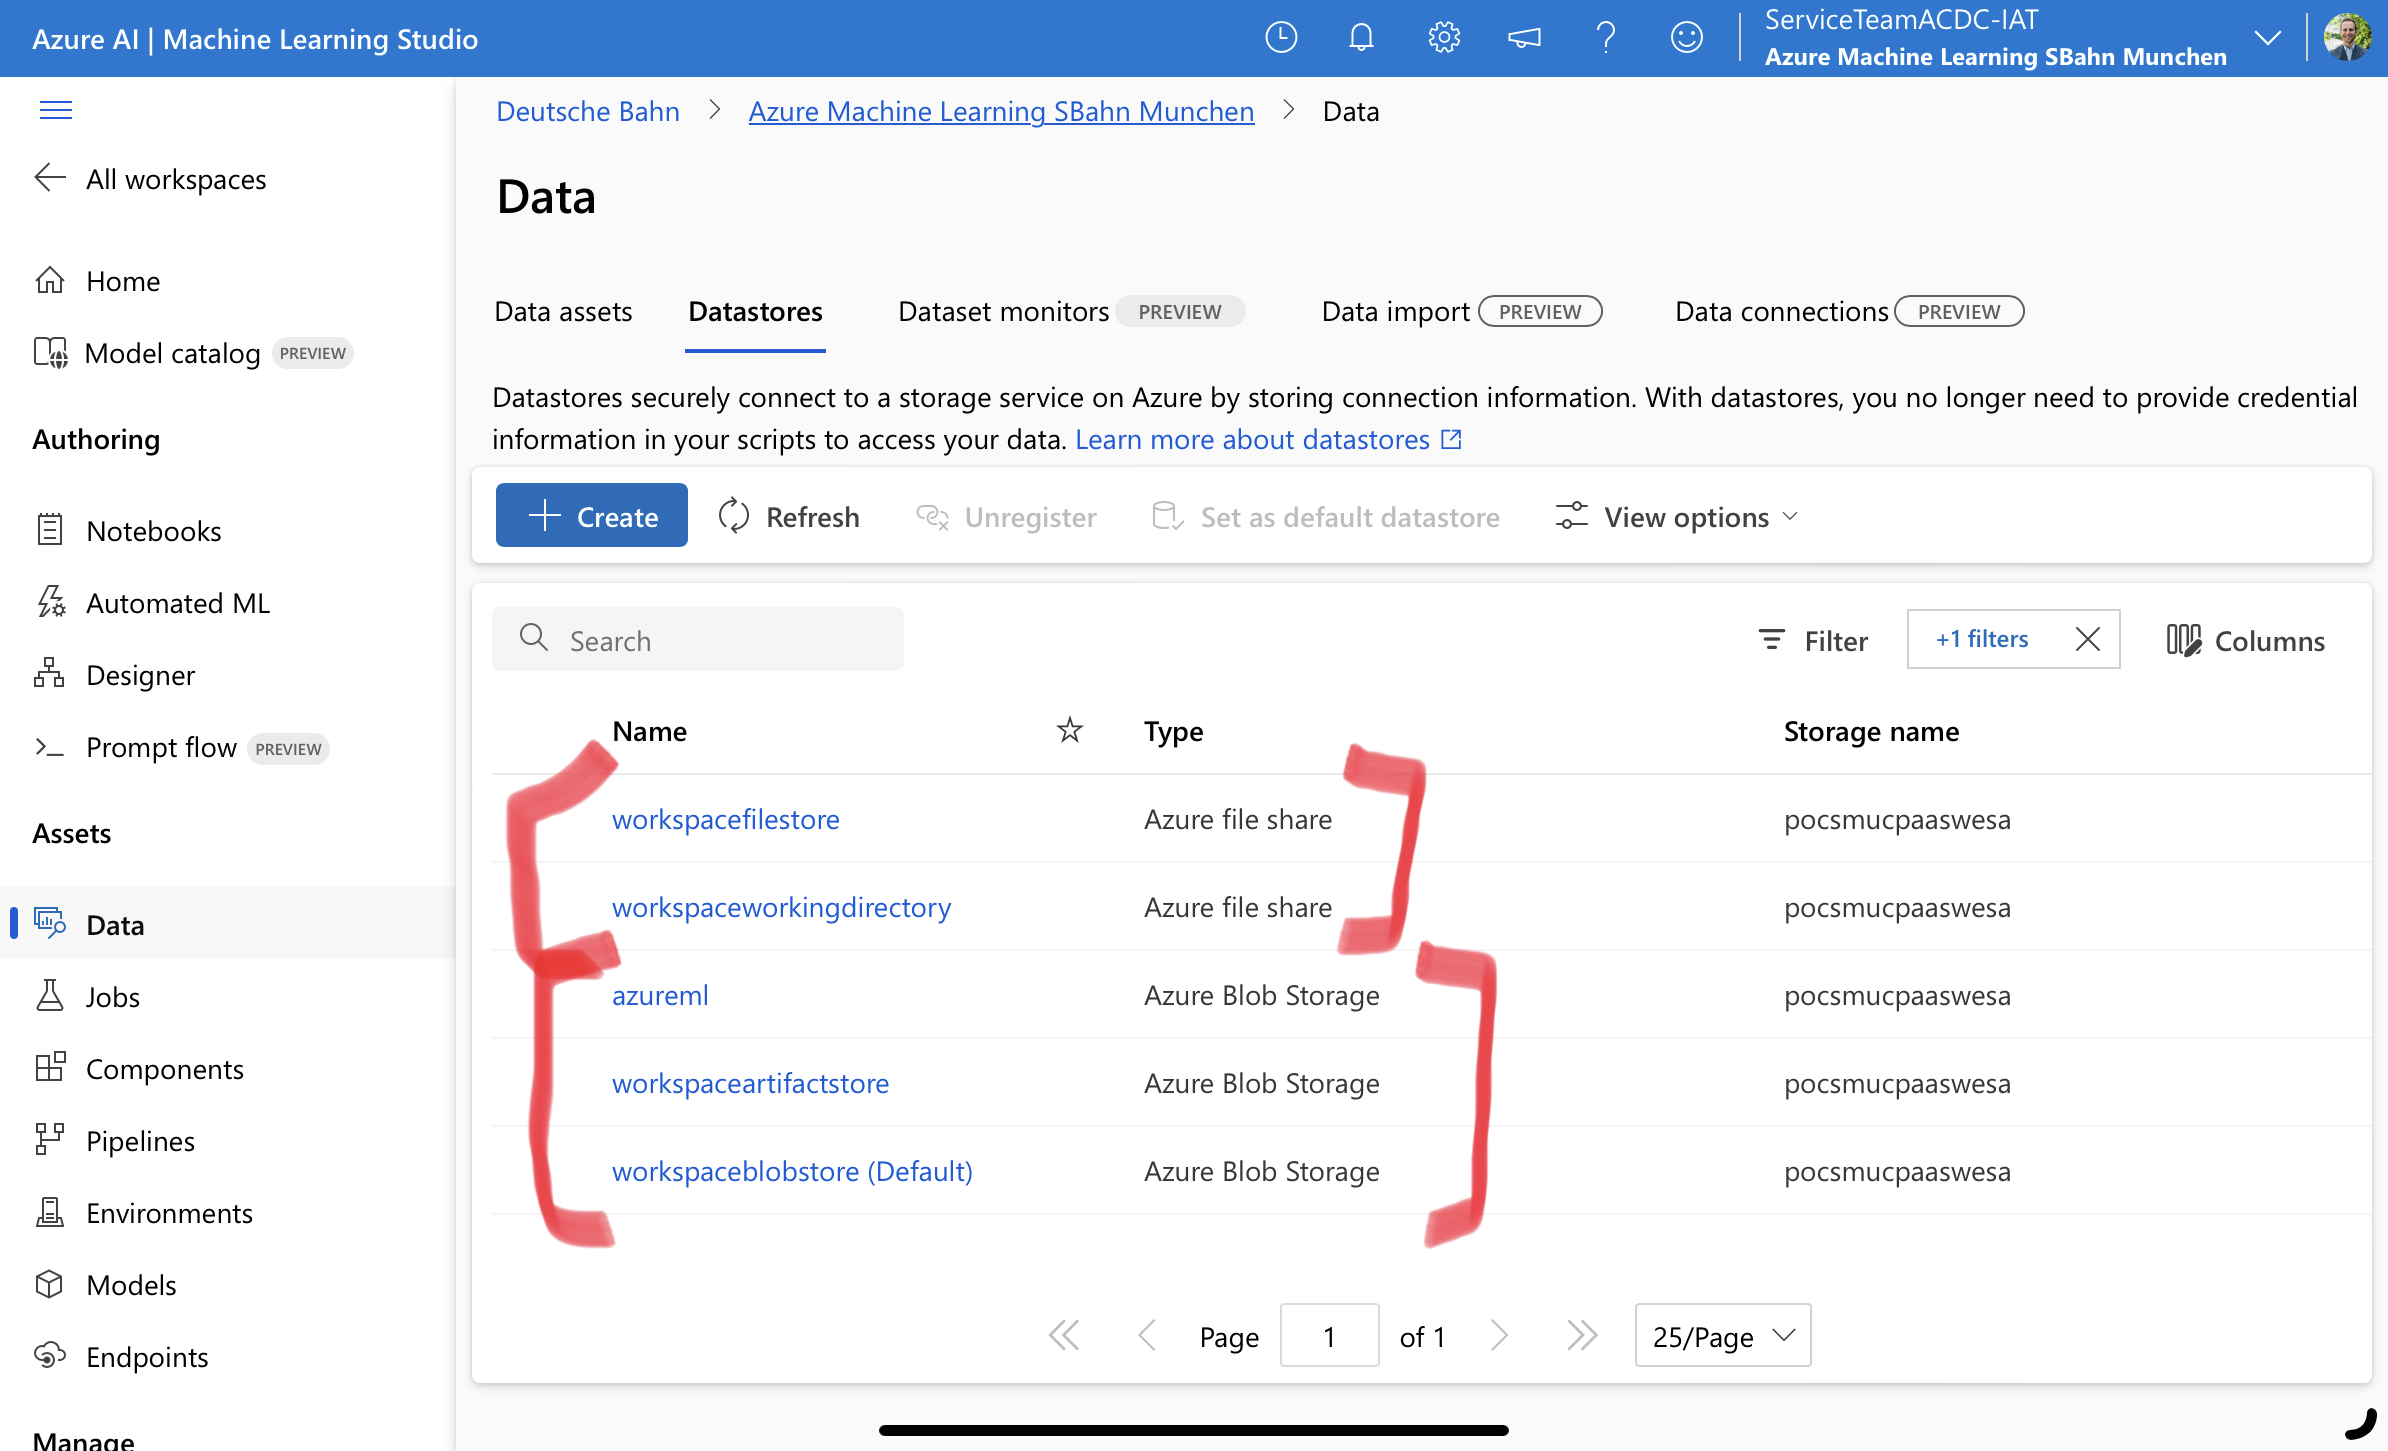
\includegraphics[scale = 0.1]{attachment/chapter_10/Scc036}
	\caption{Four seperate accounts: Two for file and for logs.}
\end{figure}

\begin{description}
	\item[workspacefilestore (filestore)] This account is normally reserved for notebooks and own created scripts. In this setup it is empty.
	\begin{figure}[H]
		\centering
		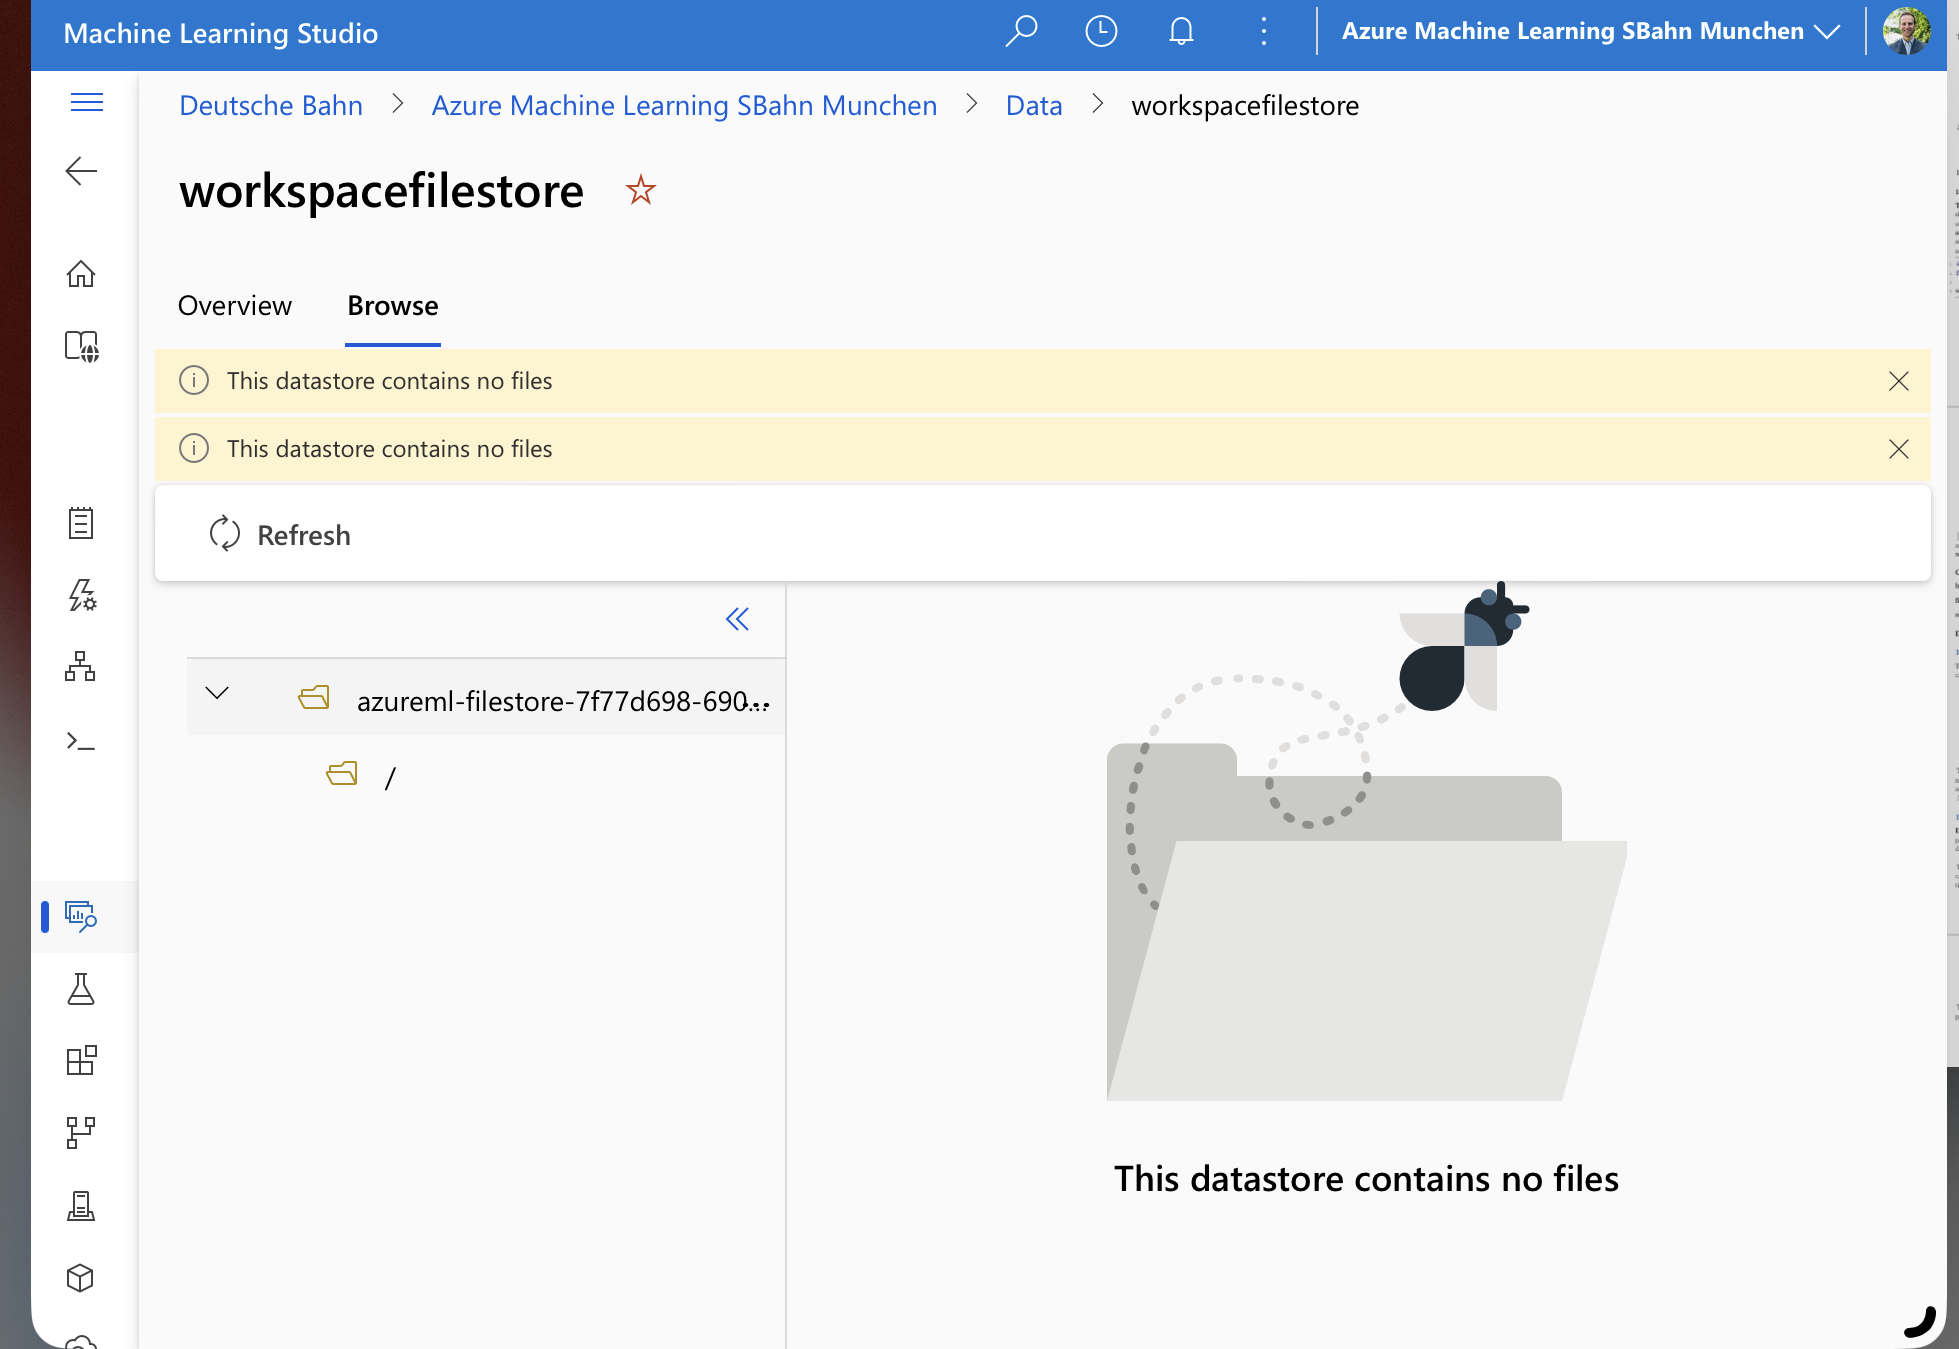
\includegraphics[scale = 0.1]{attachment/chapter_10/Scc037}
		\caption{In this setup it is empty.}
	\end{figure}
	\item[workspaceworkingdirectory (filestore)] Each user has it's own filesystem. Even each user get's created a own directly. Note: It is unclear, when exactly this happens. 
	\begin{figure}[H]
		\centering
		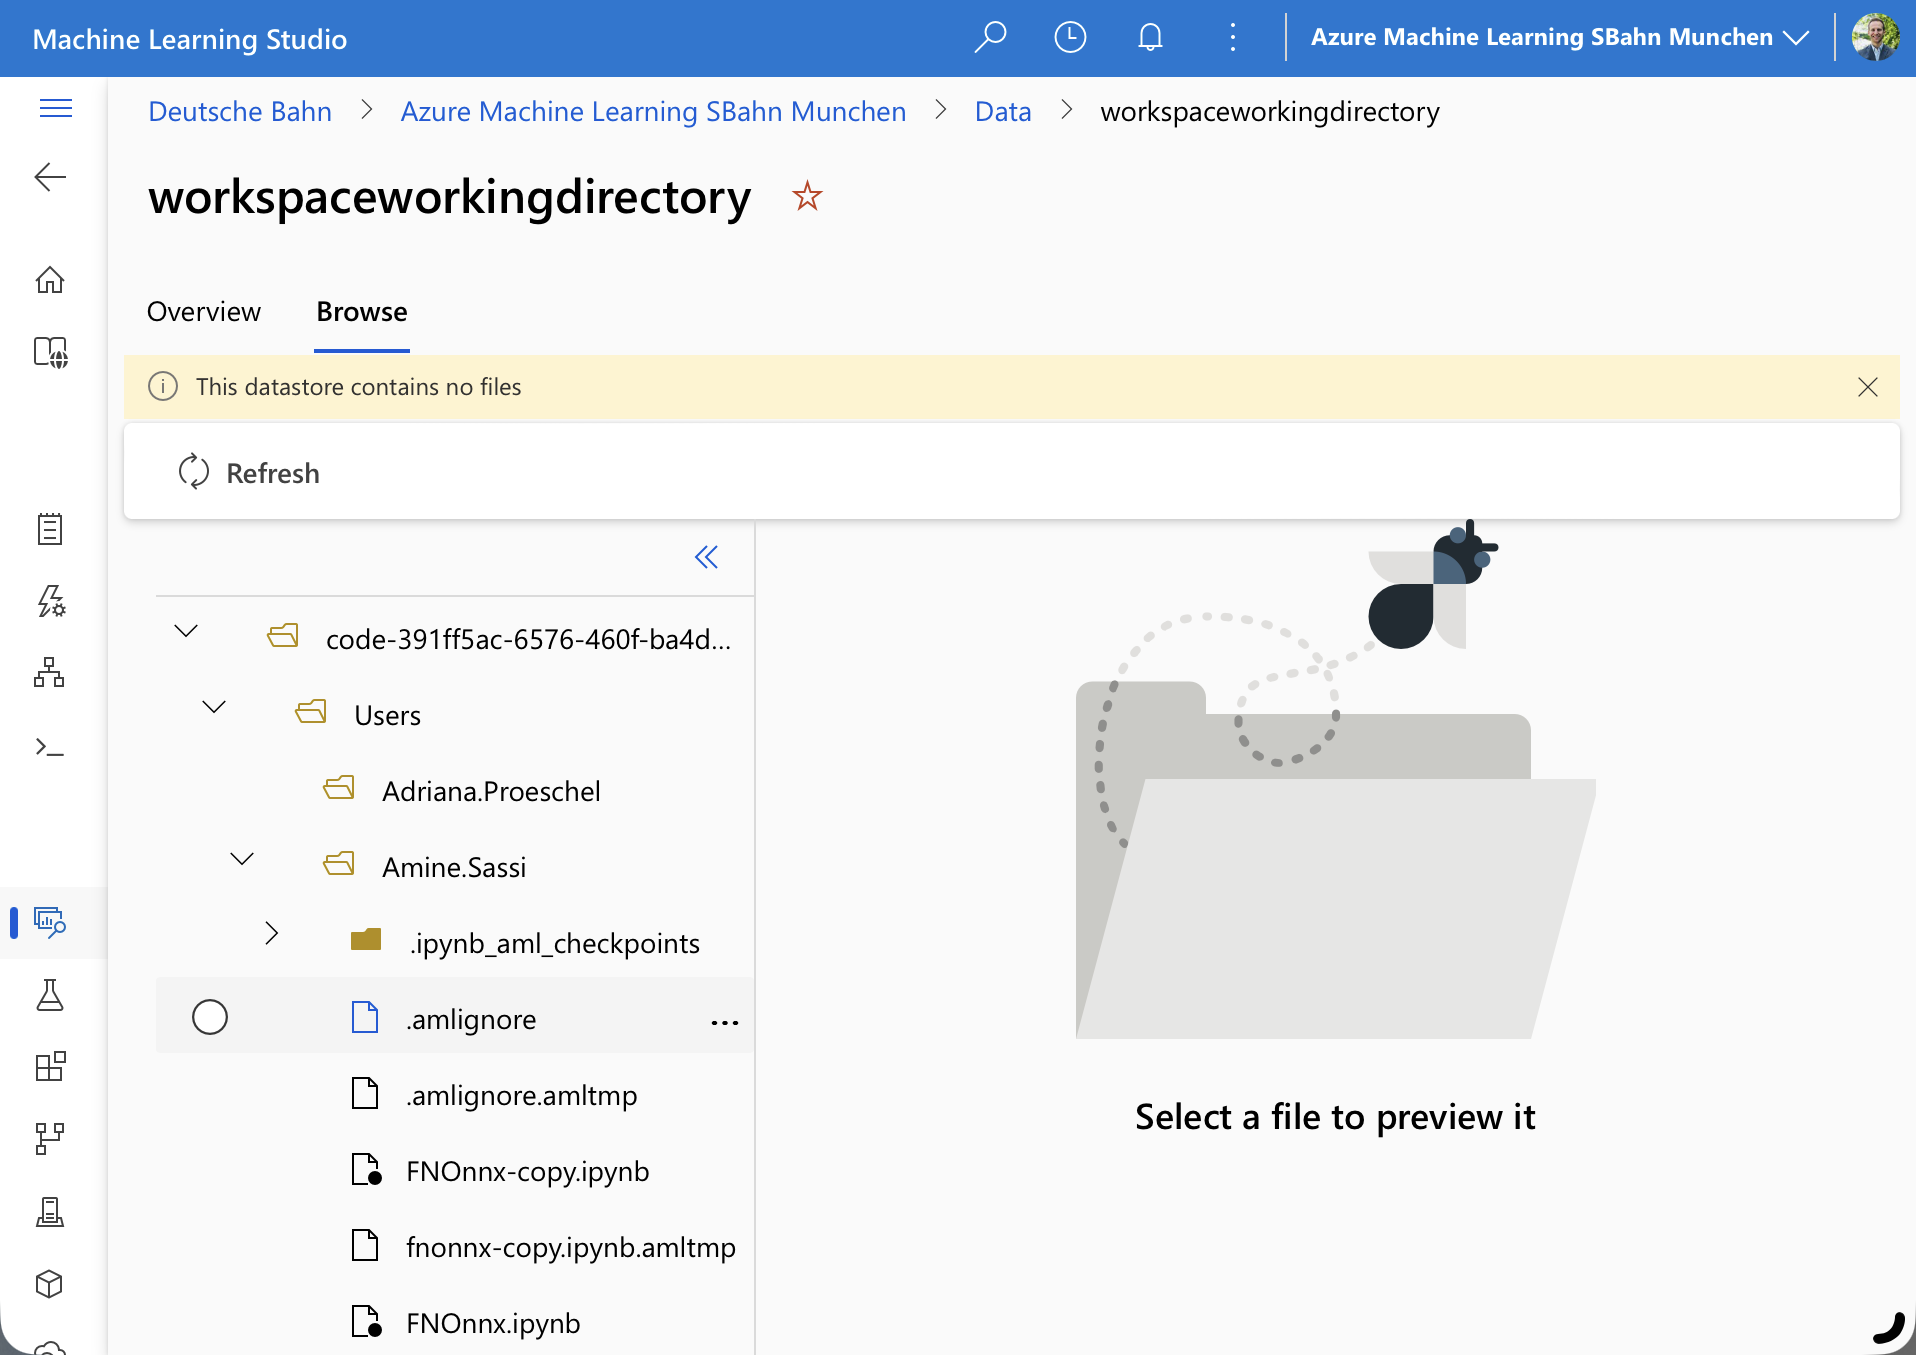
\includegraphics[scale = 0.1]{attachment/chapter_10/Scc038}
		\caption{Model/ Other own created scripts/ notebooks}
	\end{figure}
	\item[Notebook Files] as been shown, in the workspaceworking dircotry are more then just the notebook files. 
		\begin{figure}[H]
		\centering
		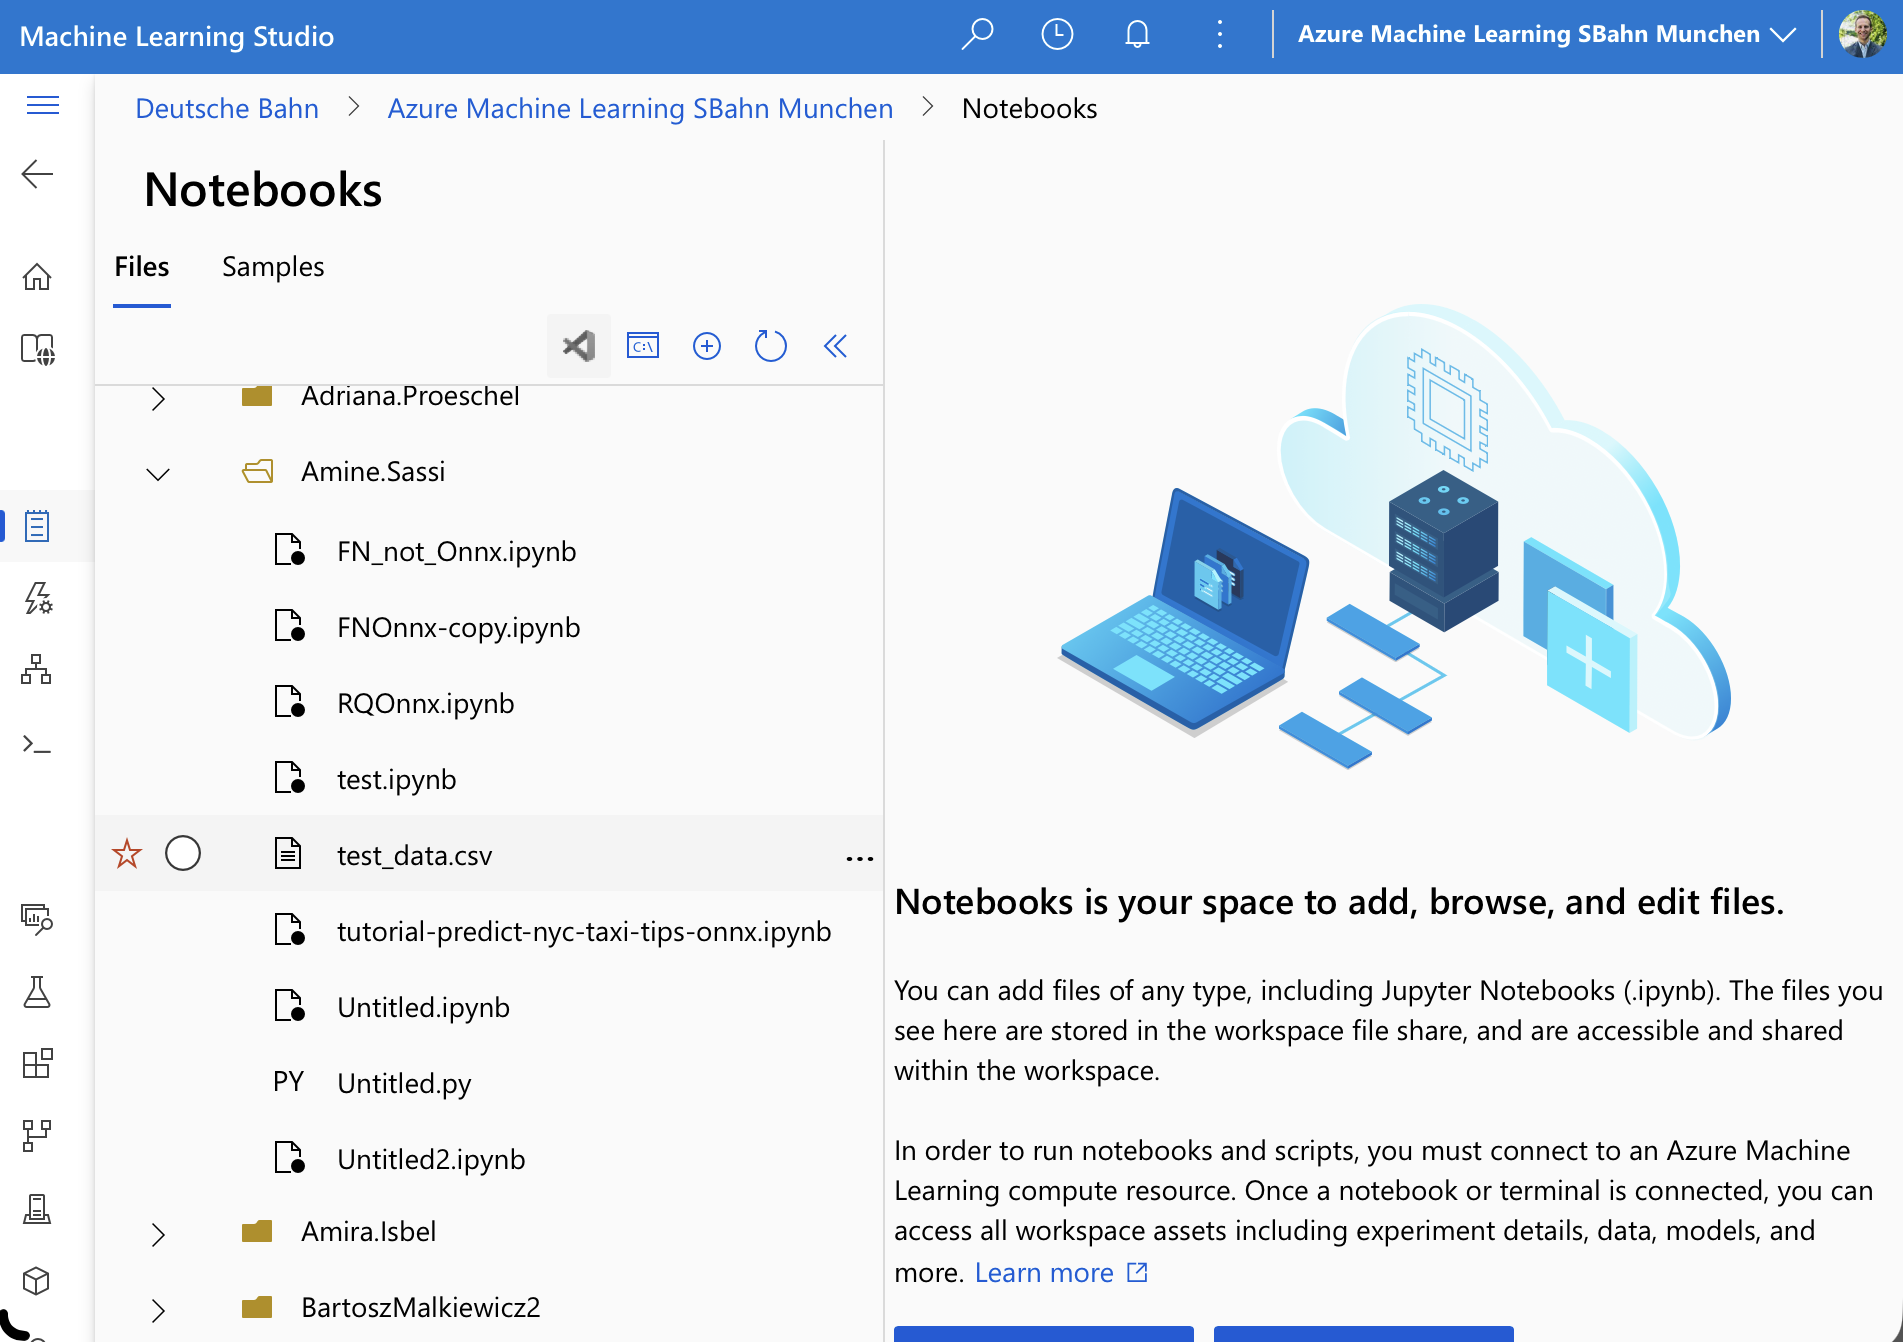
\includegraphics[scale = 0.1]{attachment/chapter_10/Scc039}
		\caption{Just Notebooks}
	\end{figure}
\end{description}

\subsubsection{Example: Blobstorage}

\begin{description}
	\item[workspaceblobstore (Default) (Store)] It looks like files, that are required to execute the pipeline or model.
	\begin{figure}[H]
		\centering
		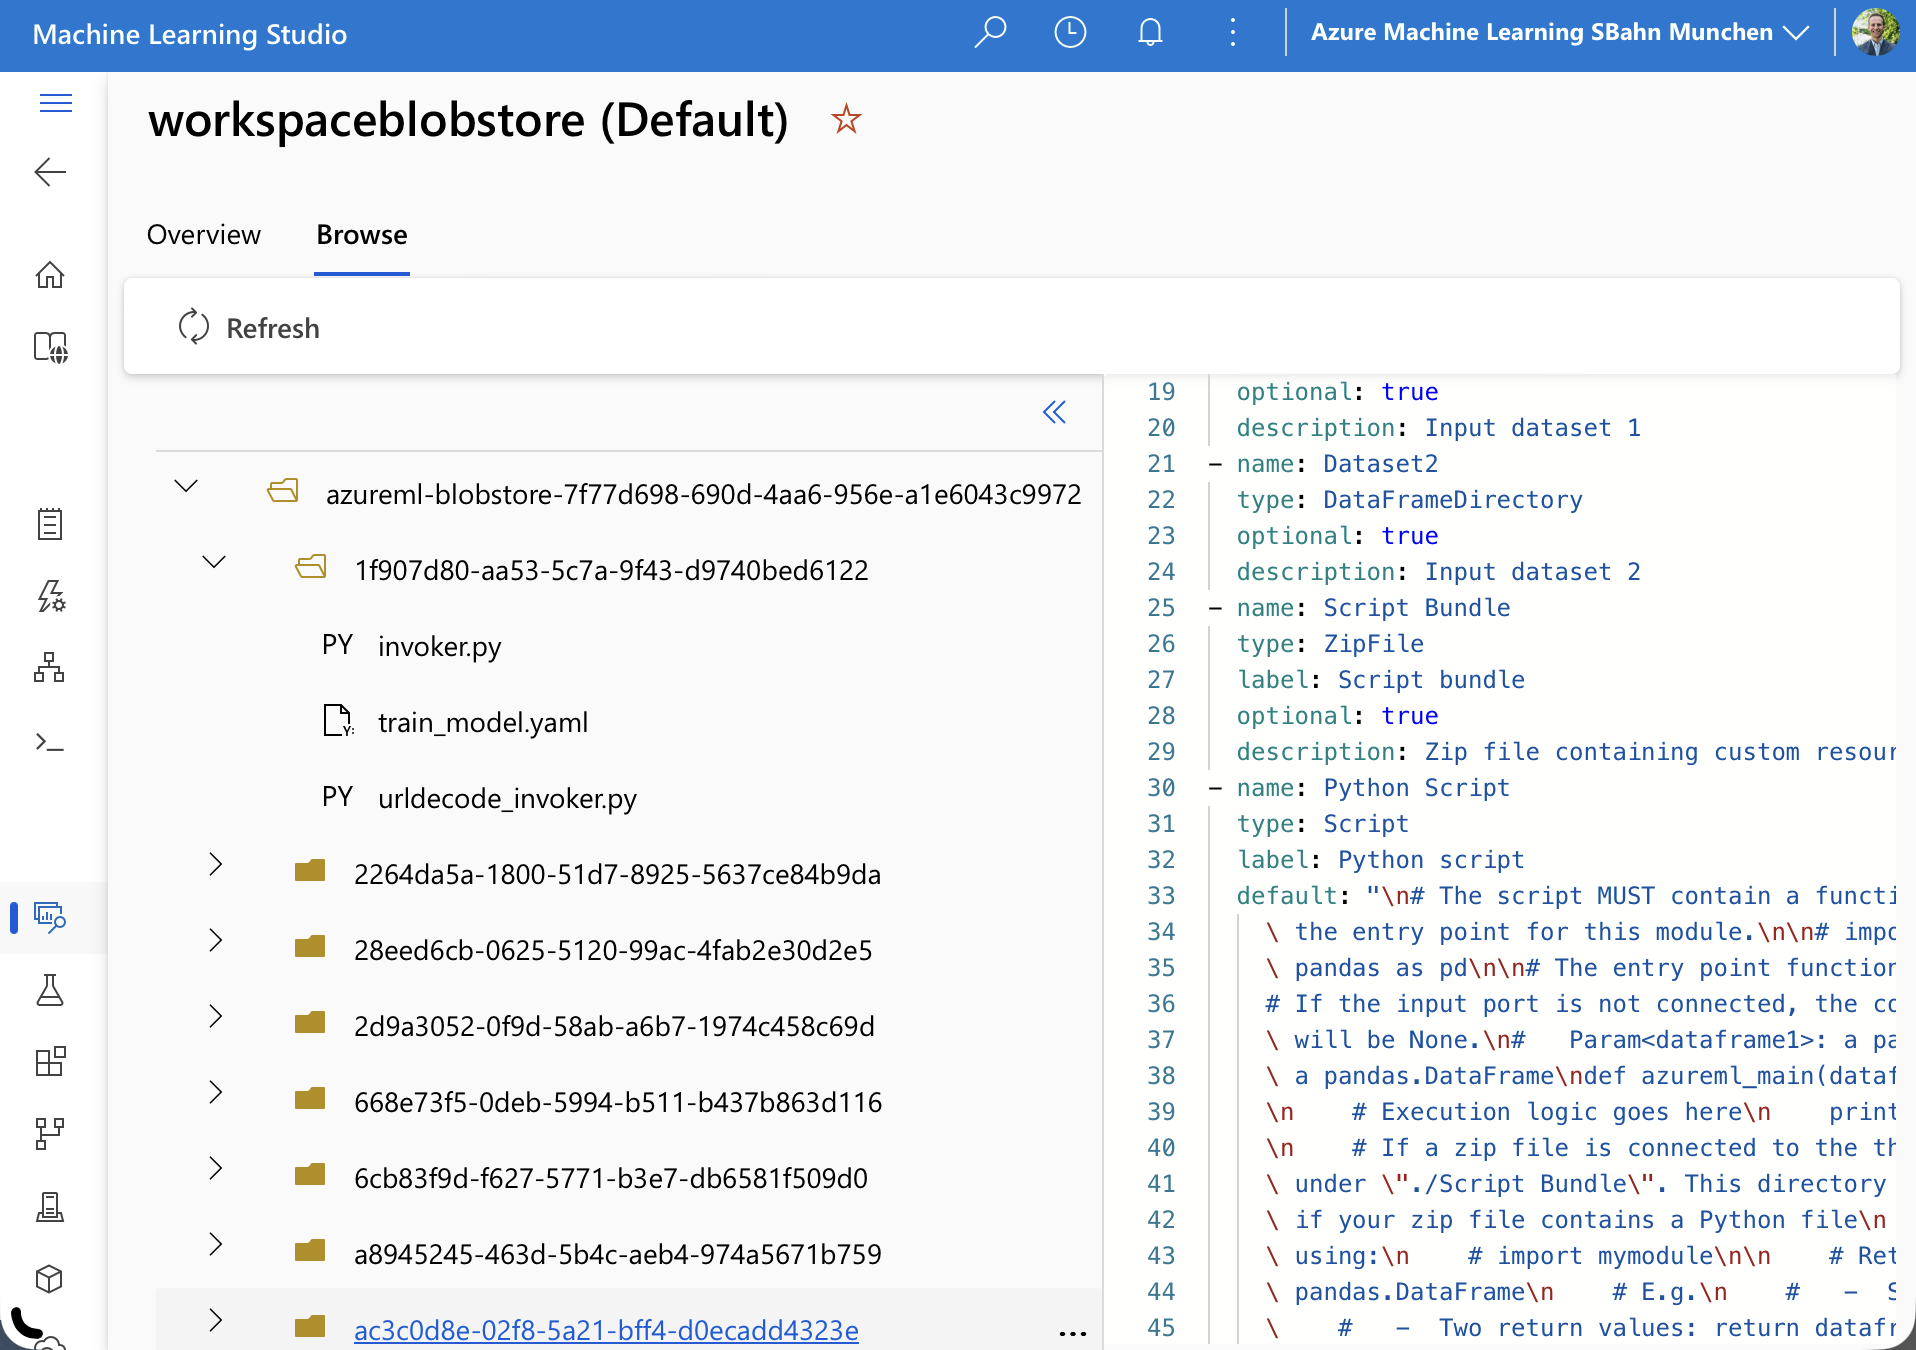
\includegraphics[scale = 0.3]{attachment/chapter_10/Scc041}
		\caption{Bit unclear, what does files are.}
	\end{figure}
	\item[worksapceartifactstore (Store)] It tracks logs for the experiment runs, compute runs and so on.
		\begin{figure}[H]
		\centering
		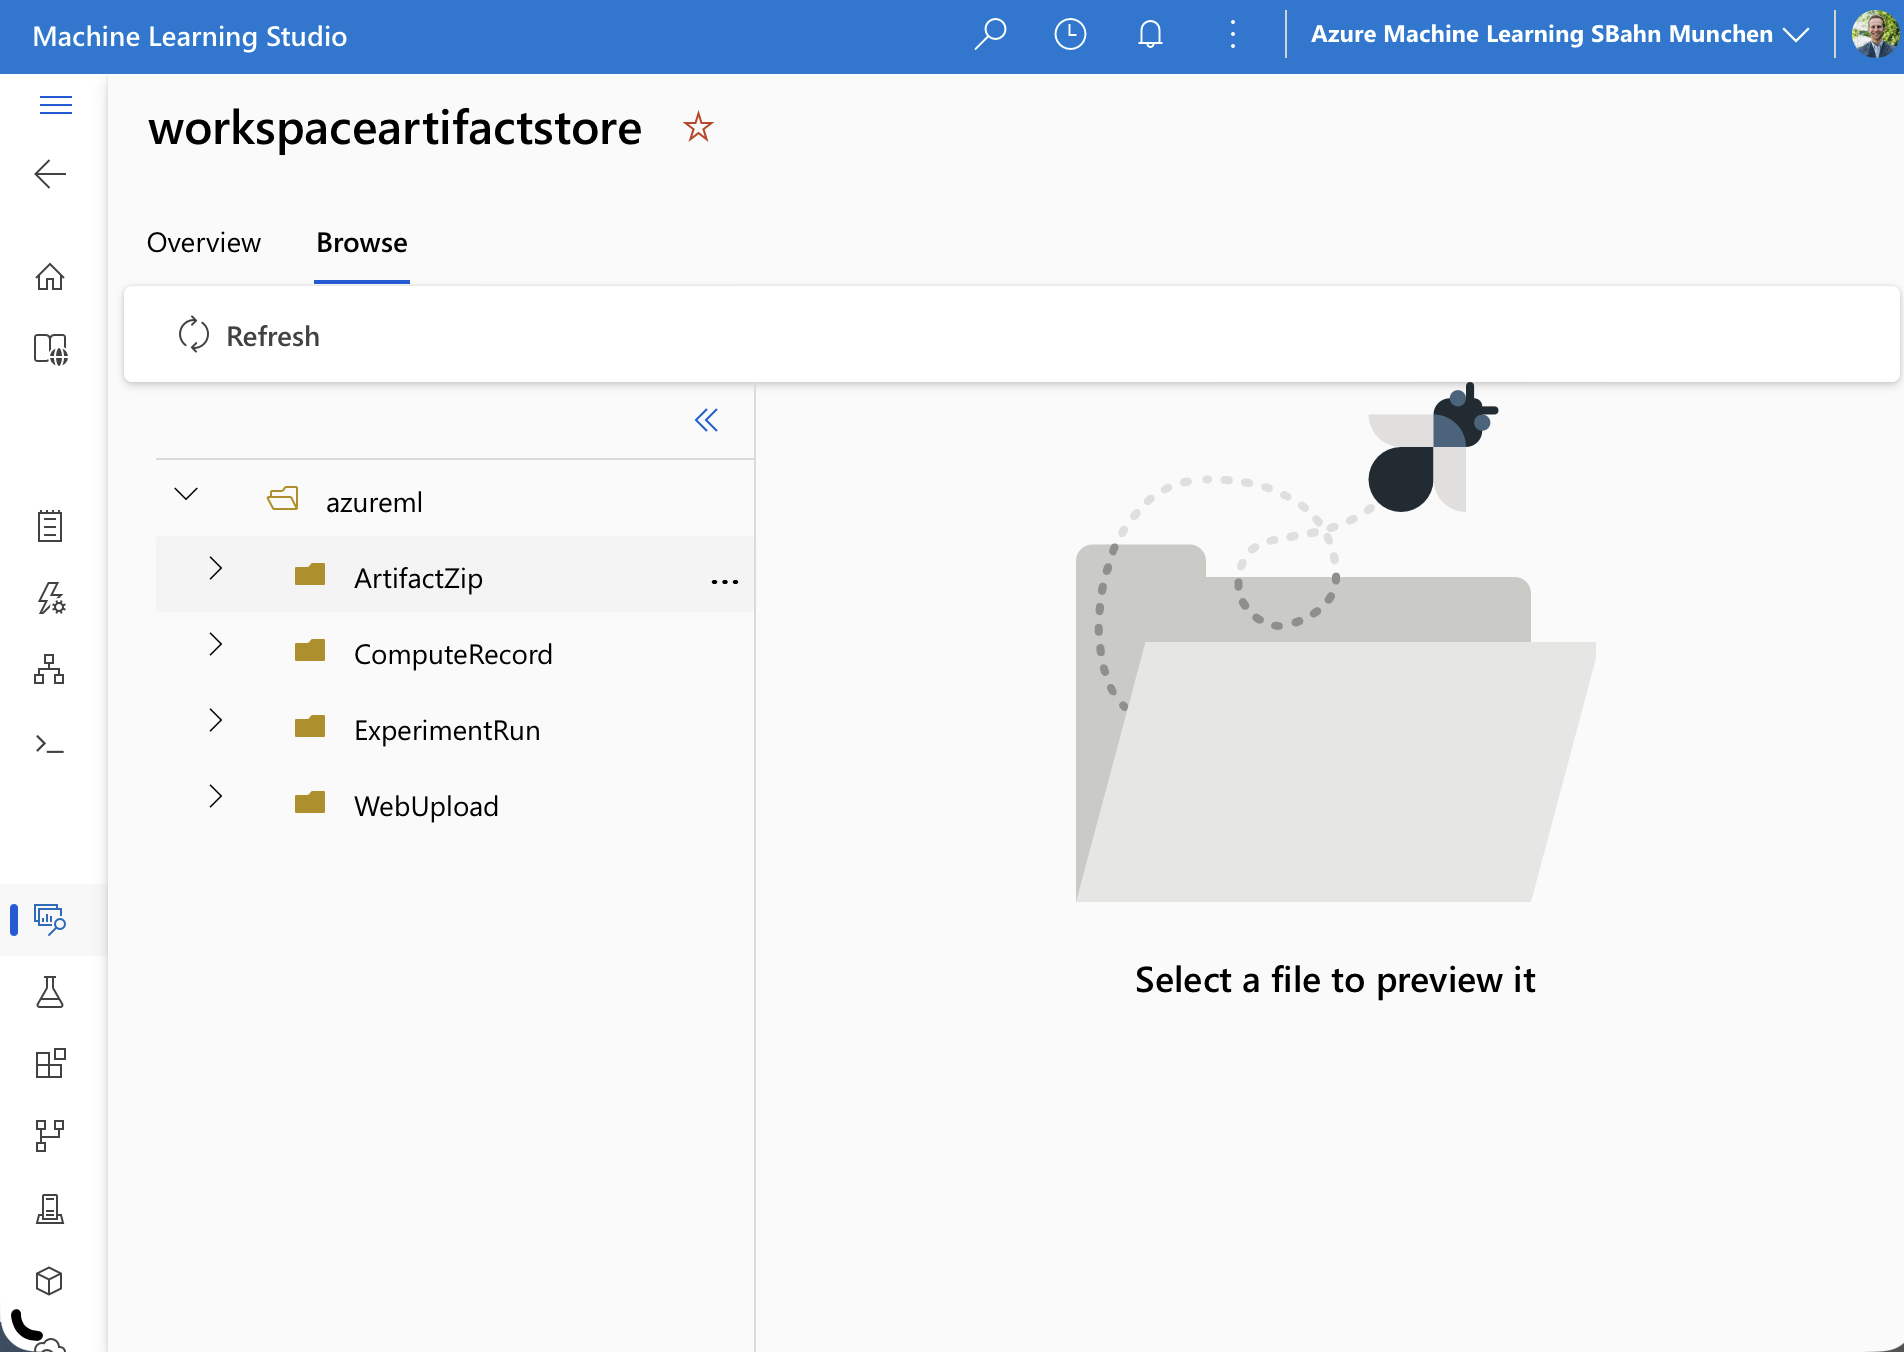
\includegraphics[scale = 0.3]{attachment/chapter_10/Scc040}
		\caption{Logging of al sorts of things}
	\end{figure}
\end{description}

\subsection{Compute Ressources}
The compute ressources which are needed for a explore data analysis, training or inferenceing can be managed directly in Azure ML. For this a \gls{VM} is spindup.\\

\begin{figure}[H]
	\centering
	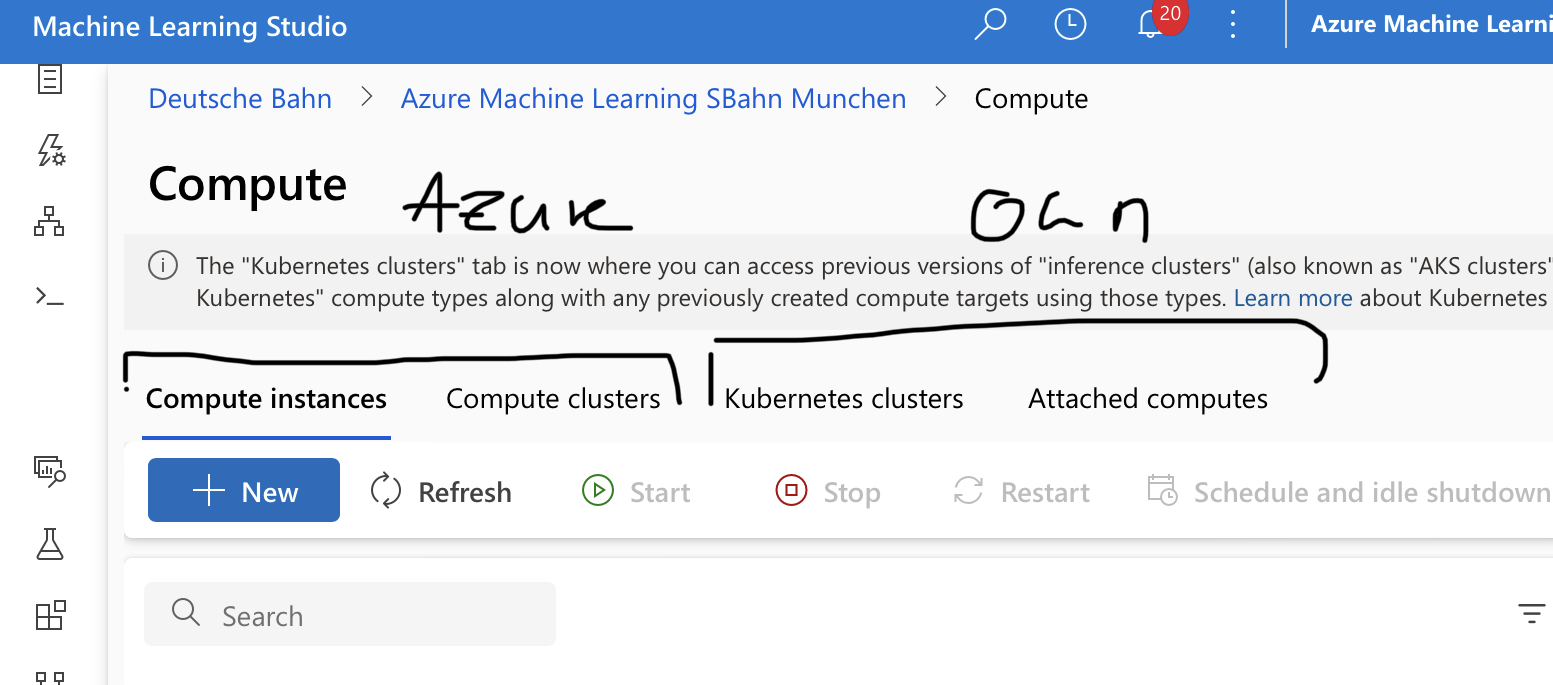
\includegraphics[scale = 0.1]{attachment/chapter_10/Scc030}\\ 
	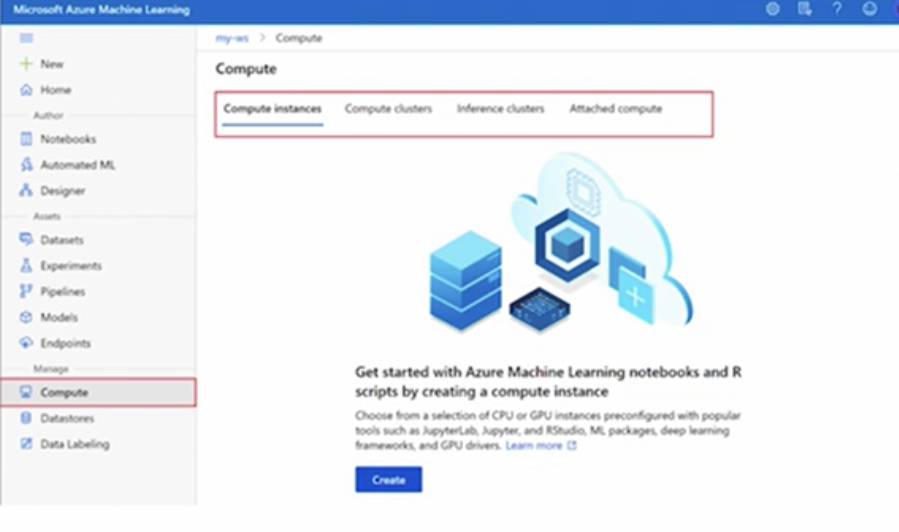
\includegraphics[scale = 0.1]{attachment/chapter_10/Scc031}
	\caption{Compute Types}
\end{figure}

\begin{itemize}
	\item The \textit{compute instance}/ \textit{compute cluster} is on or multiple \gls{VM}   for research and training the model.
	\item Also can be attached own \gls{VM}. 
	\item The field \textit{inference cluster} or new \textit{Kubernets cluster} allows to bring own cluster for the deployment process.
\end{itemize}


\textit{Note} For deployment with managed endpoints the this is spin up by it self.

\subsection{Model}
\subsubsection{Difference between ML and traditional Software}
In the traditional programming a problem is adressed, by having input data and designing a programm, which transforms this data to a desired output. The logic is hard coded.\\ 

With \gls{ML} a $"$Model$"$ derives the logic form the input and combined output data. This logic can be updated - trained over time. The model is the \textit{anwser} to the problem. Most of the time, it is unclear, why, but the evaluation of the model takes care of this.

\begin{figure}[H]
	\centering
	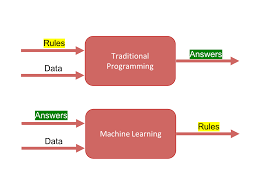
\includegraphics[scale = 0.1]{attachment/chapter_10/Scc034.PNG}
	\caption{Output is a Model}
\end{figure}

The learned model is trained on input and output data. This is then deployed as the $"$traditional$"$ programm.

\begin{figure}[H]
	\centering
	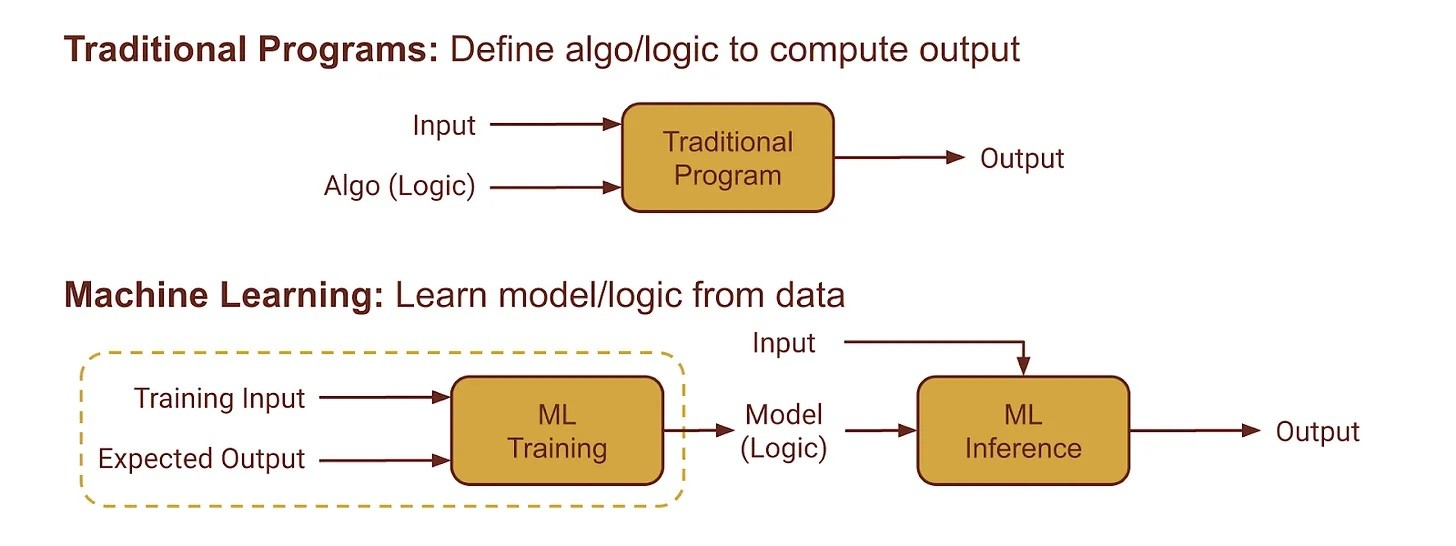
\includegraphics[scale = 0.1]{attachment/chapter_10/Scc035.JPG}
	\caption{Deployment of the Model}
\end{figure}

\subsection{Pipelines Designer}
\subsubsection{Example: Simple Model}
A no-code option is \textit{Designer}. It allows for a click-drop design of the process. From 
\begin{itemize}
	\item data ingestion,
	\item training,
	\item scoring
	\item to validating
\end{itemize}
the process steps can be selected by linked modules.

\begin{figure}[H]
	\centering
	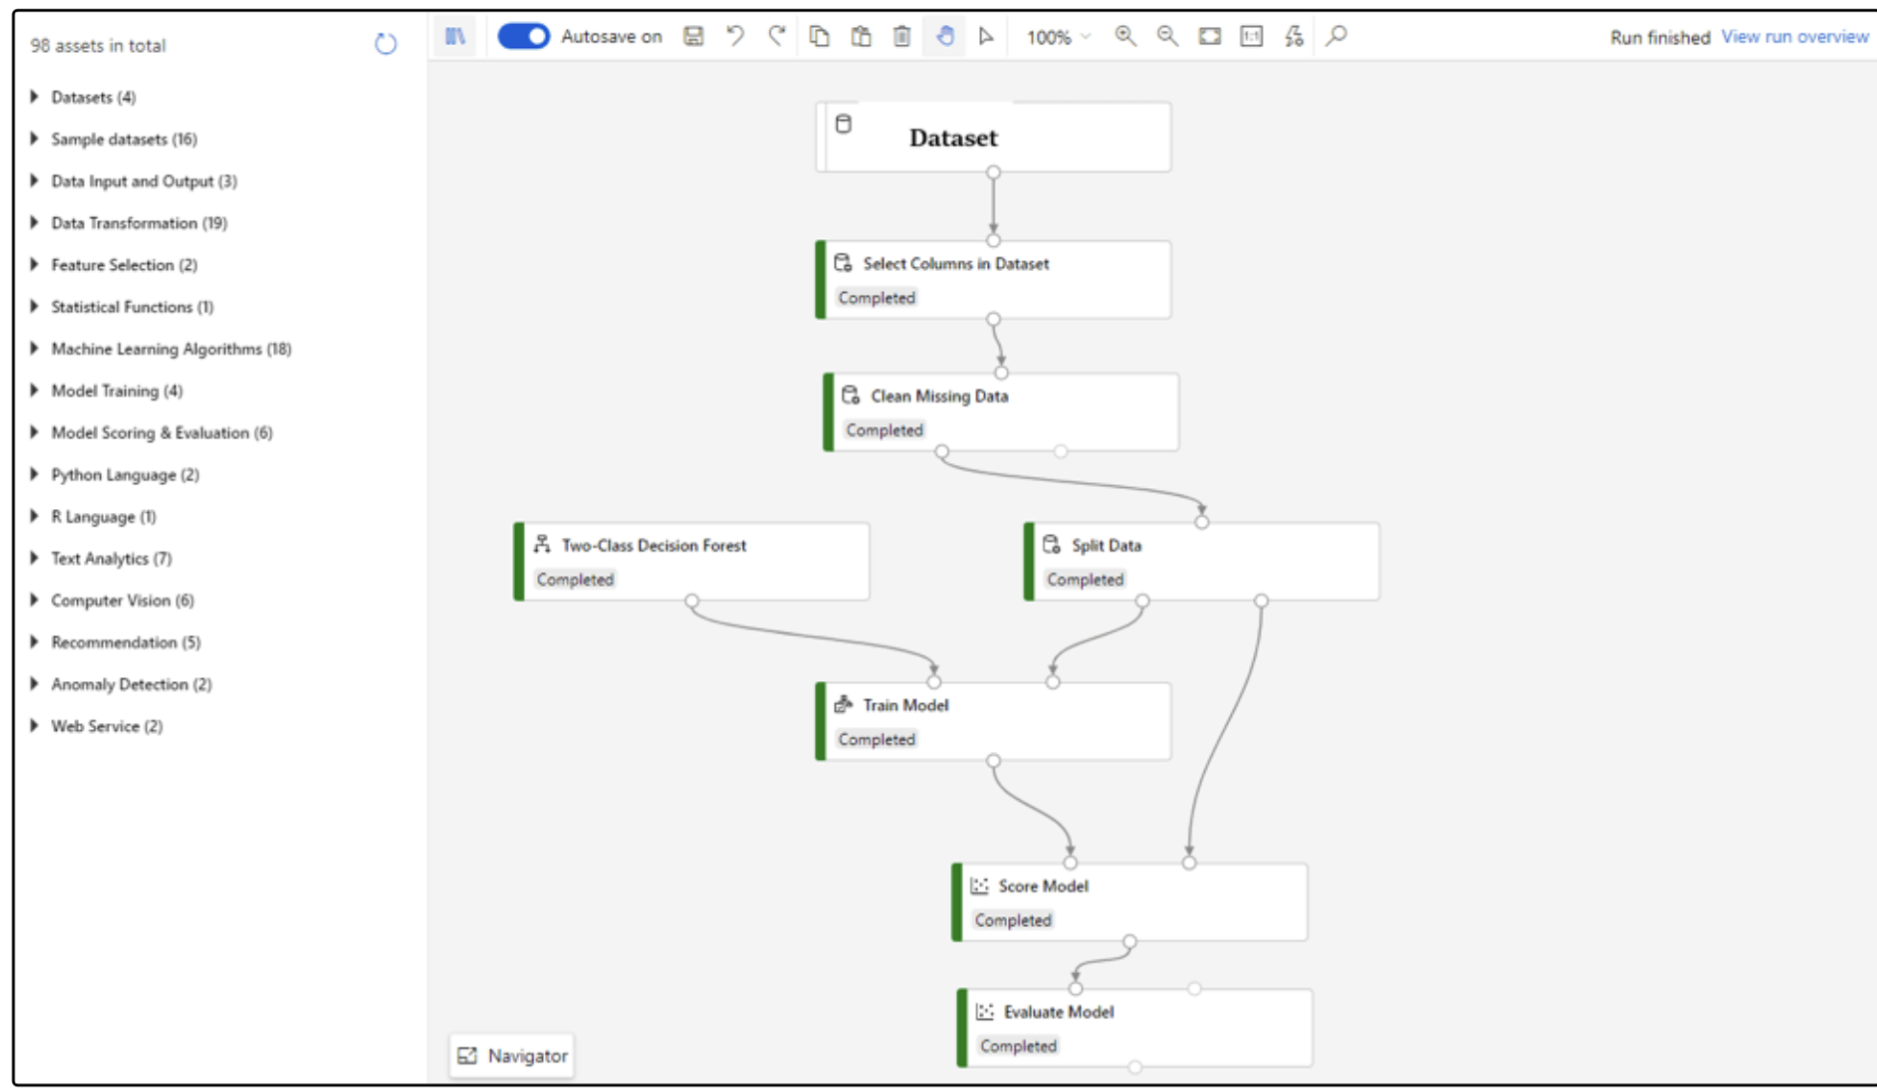
\includegraphics[scale = 0.3]{attachment/chapter_10/Scc005}
	\caption{Example Process}
\end{figure}

In this simple example a model will be a part of the pipeline. The steps in a \gls{ML} process are finding the right feature, cleaning the data, then spliting the data, train a model with a algorithm as a input and then score the rest of the dataset (splited), which was not used for training the model. The results of the scored data are then evaluated.

\subsection{Notebooks}
\subsubsection{git repo Integration}
It is possible to clone a repo into \textit{workspacefilestorage}. This is done over the terminal function.

\begin{figure}[H]
	\centering
	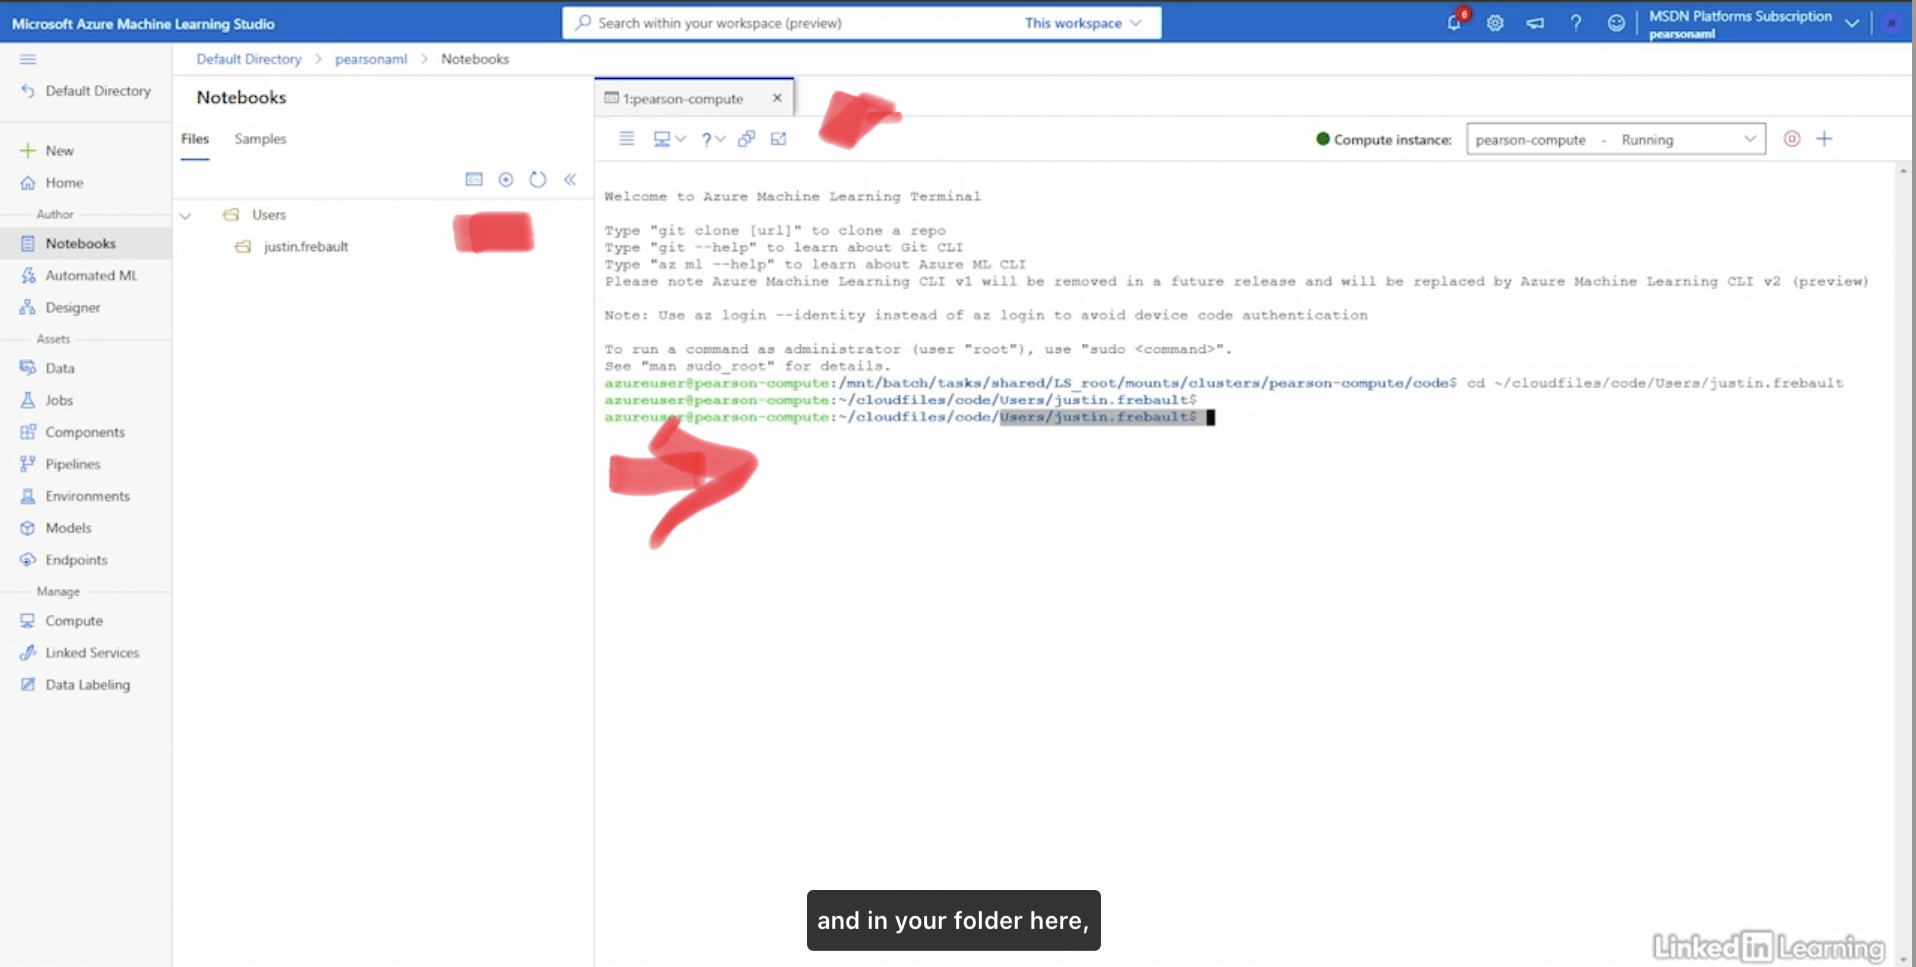
\includegraphics[scale = 0.2]{attachment/chapter_10/Scc042}
	\caption{Open Terminal}
\end{figure}

Provides with the url of the repo, this can be cloned into the filesystem. 
\begin{lstlisting}[style=CMD]
	git clone https://gitlab.com/justin.frebault/pearson-course-aml
\end{lstlisting}

\begin{figure}[H]
	\centering
	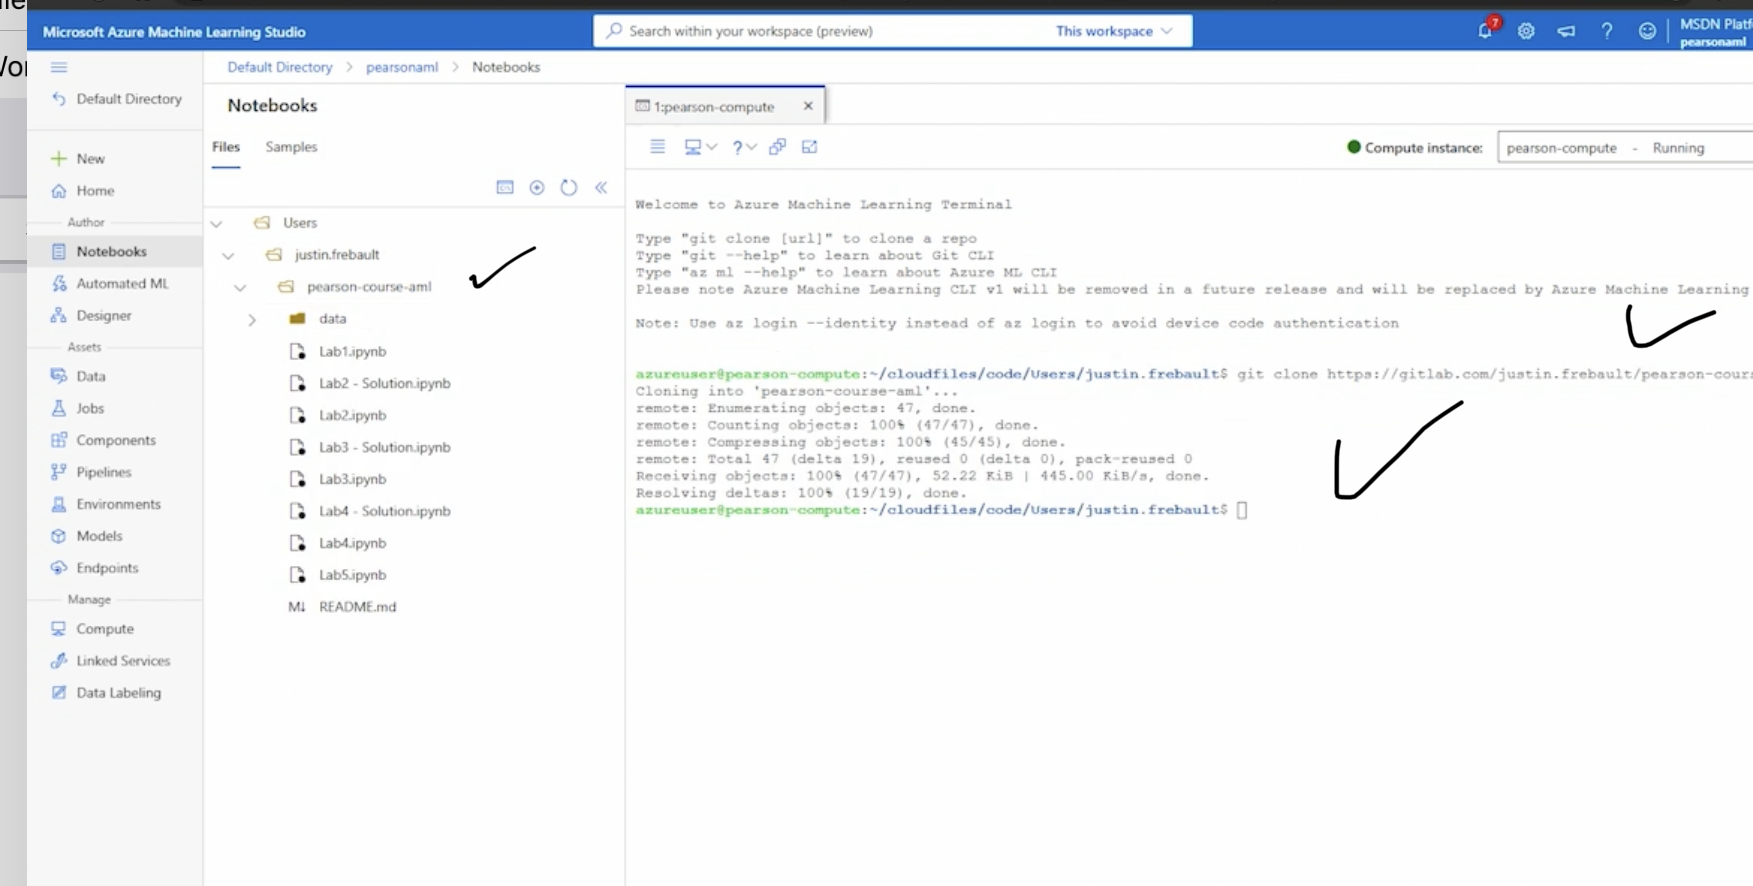
\includegraphics[scale = 0.3]{attachment/chapter_10/Scc043}
	\caption{Clone Repo}
\end{figure}

\textit{Note:} The file is only for testing. The filestorage account is not for storing data. In the workspacefile storage account is the full view of all the files for the cloned repo.

\begin{figure}[H]
	\centering
	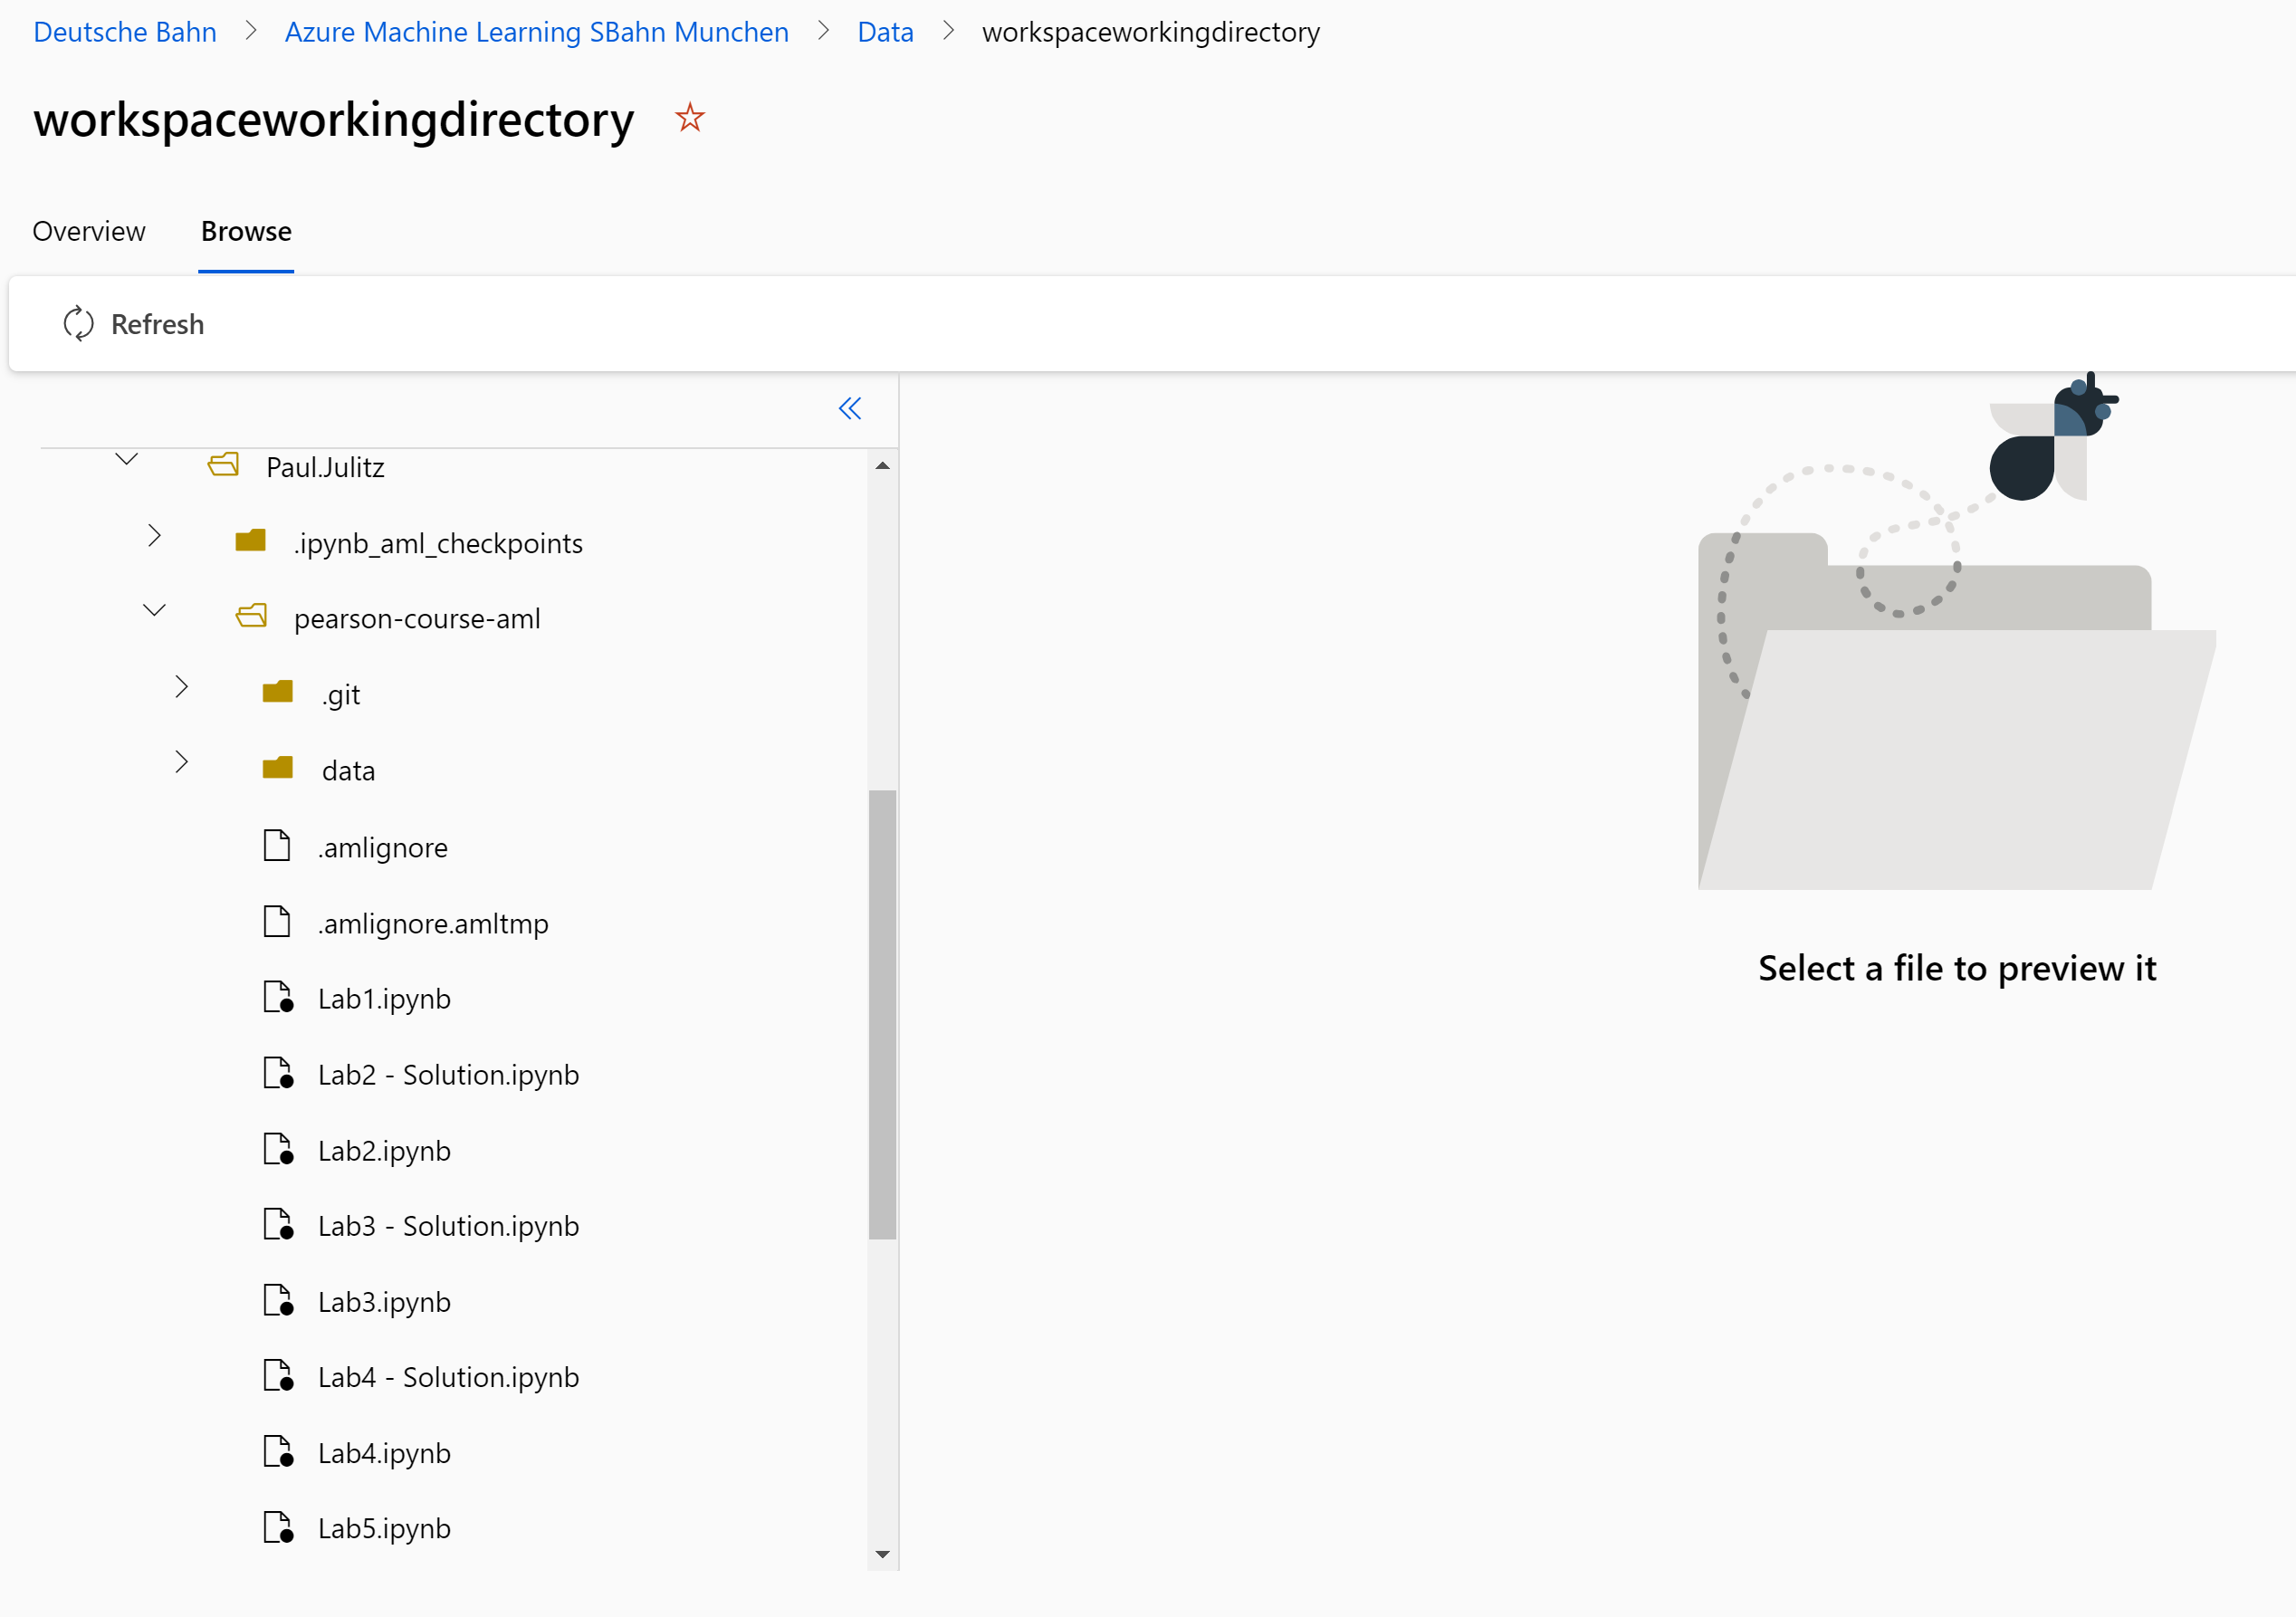
\includegraphics[scale = 0.3]{attachment/chapter_10/Scc045}
	\caption{View over data storage}
\end{figure}


\begin{figure}[H]
	\centering
	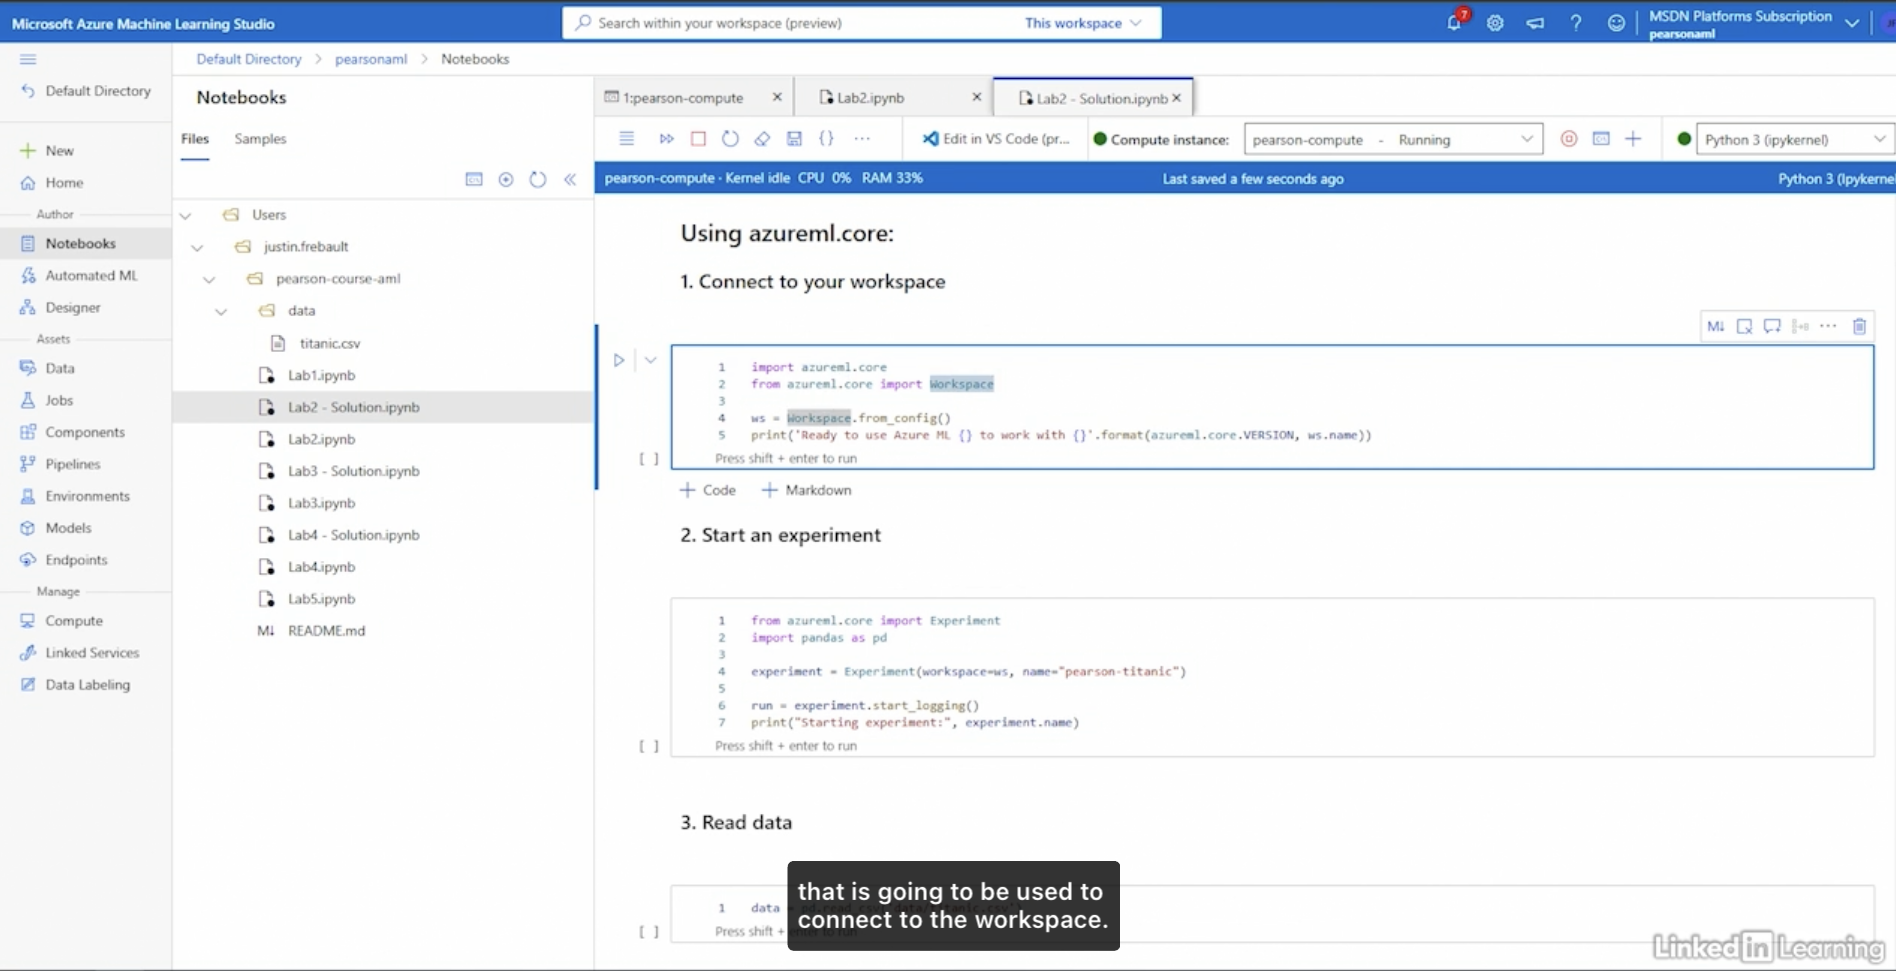
\includegraphics[scale = 0.3]{attachment/chapter_10/Scc044}
	\caption{Connecting to the data source}
\end{figure}

\subsubsection{Using VStudio Code}
The notebook can also be used and accessed with \textit{VStudio Code (Desktop)} or \textit{VStudio Code (Browser)}.

\begin{figure}[H]
	\centering
	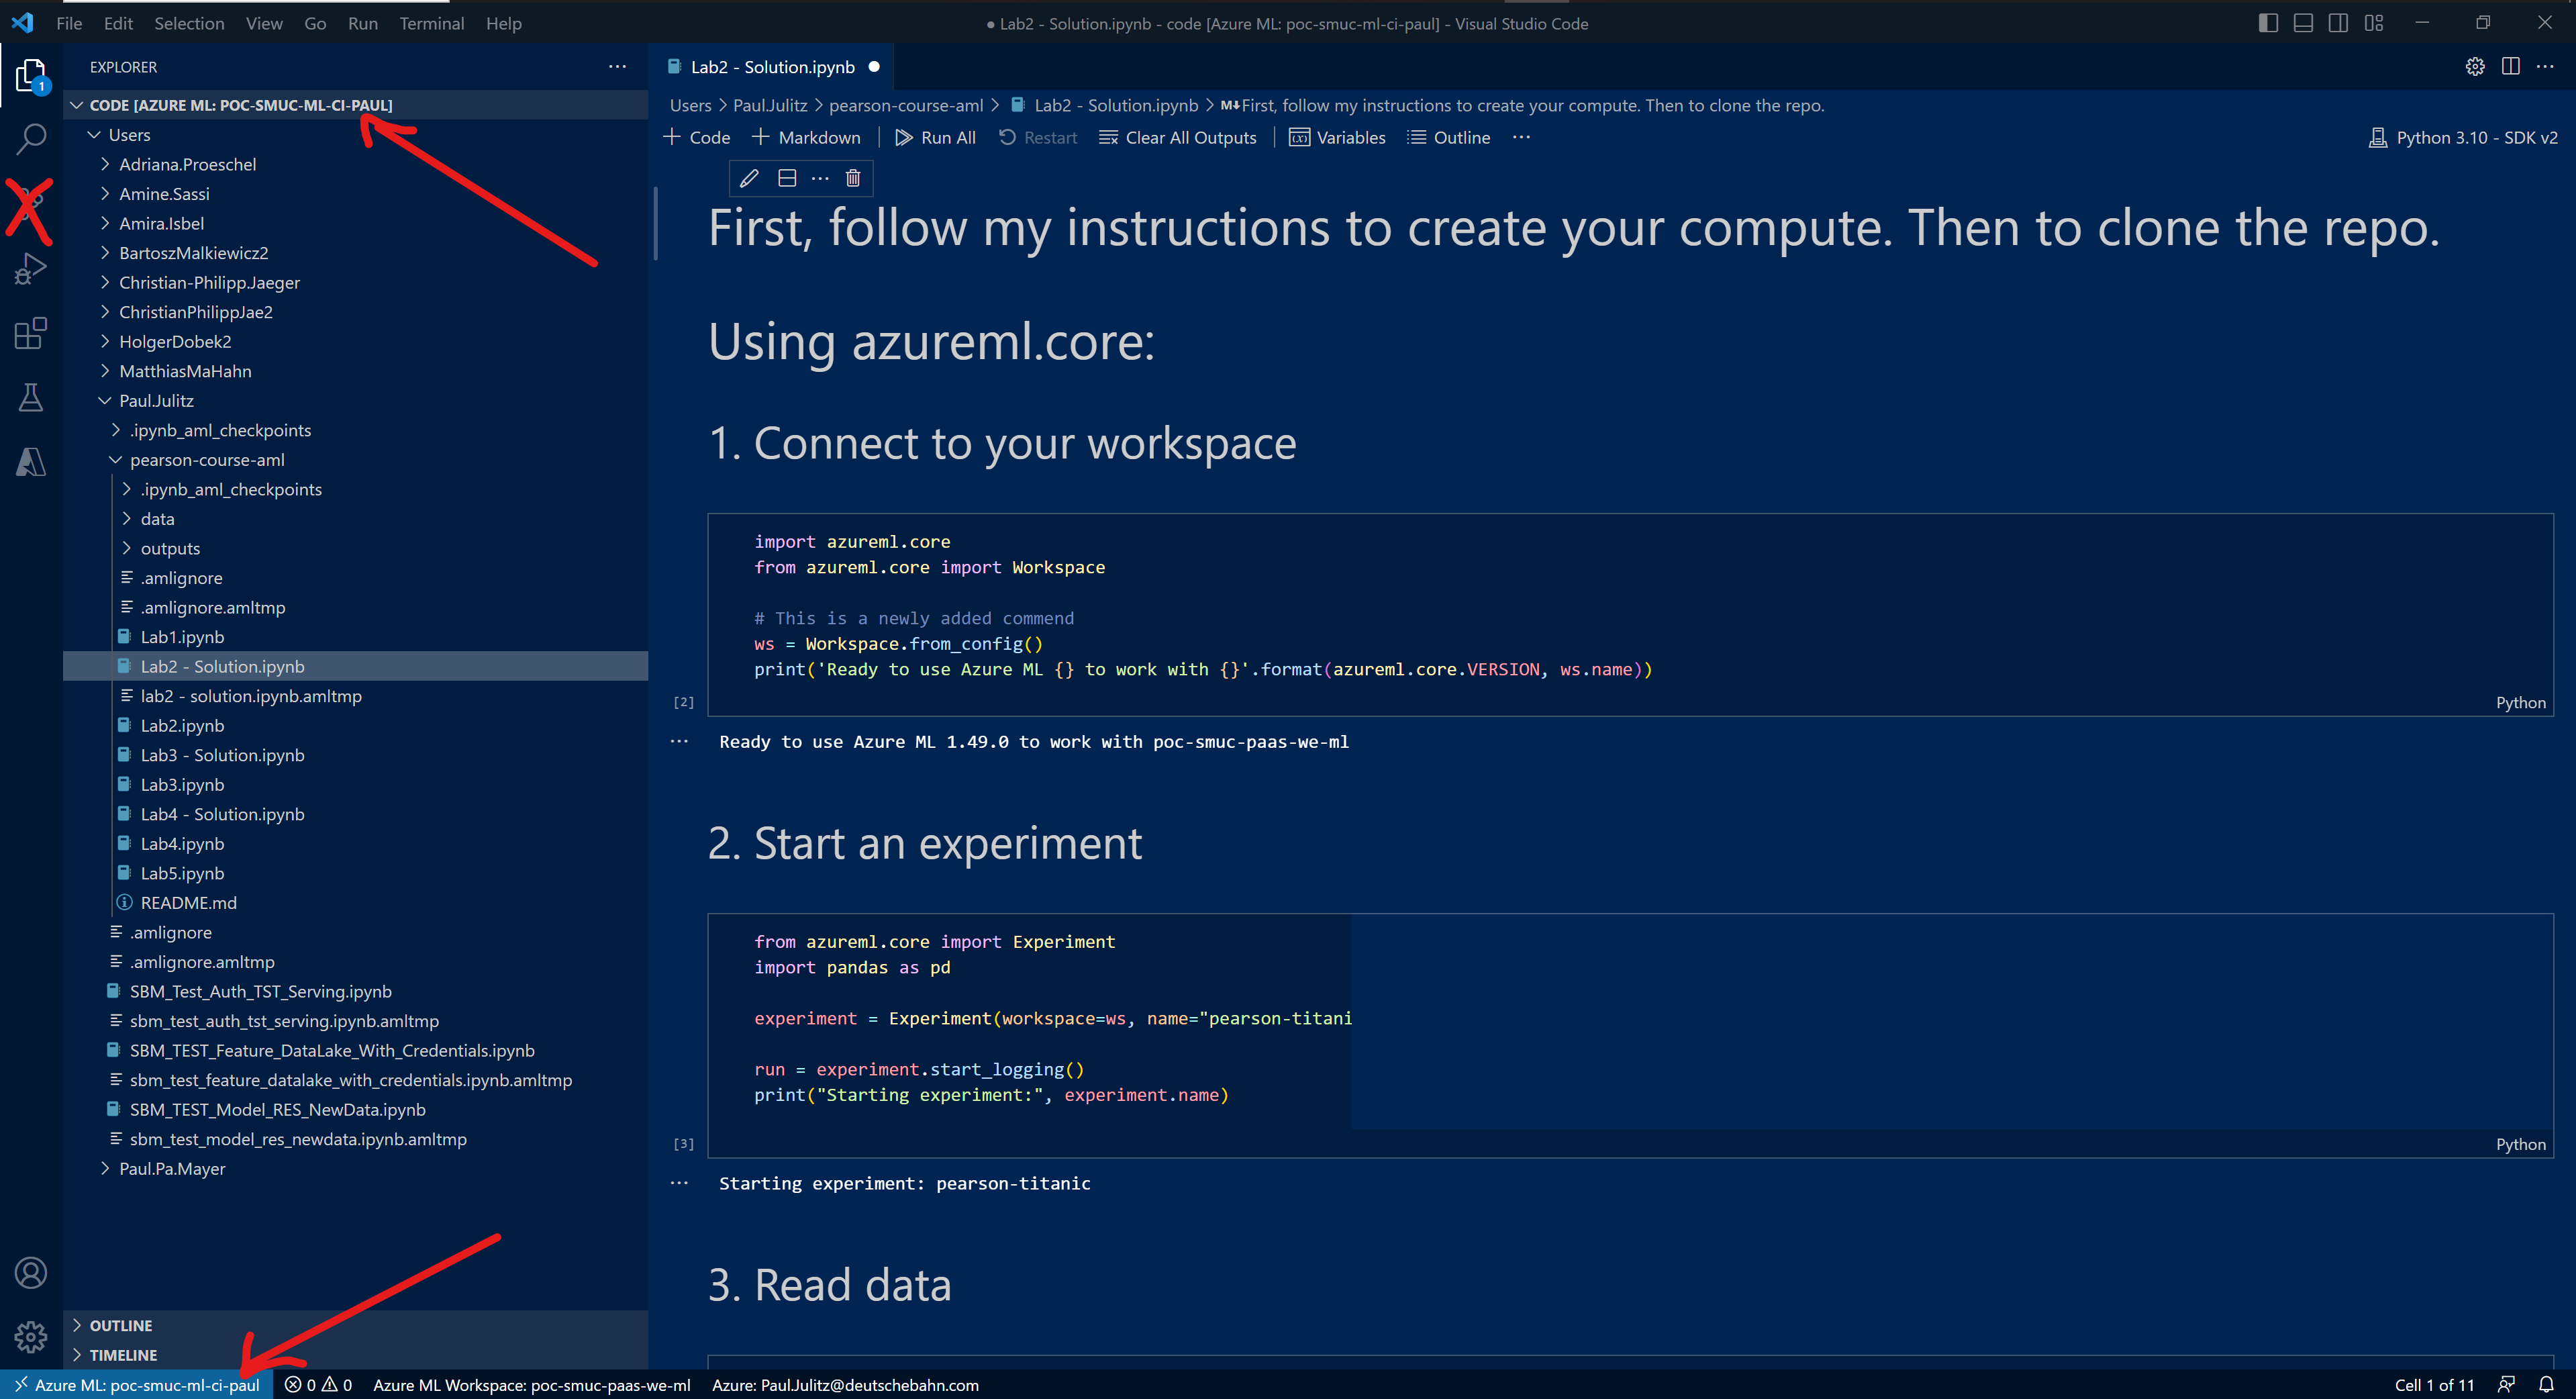
\includegraphics[scale = 0.1]{attachment/chapter_10/Scc048}\\
	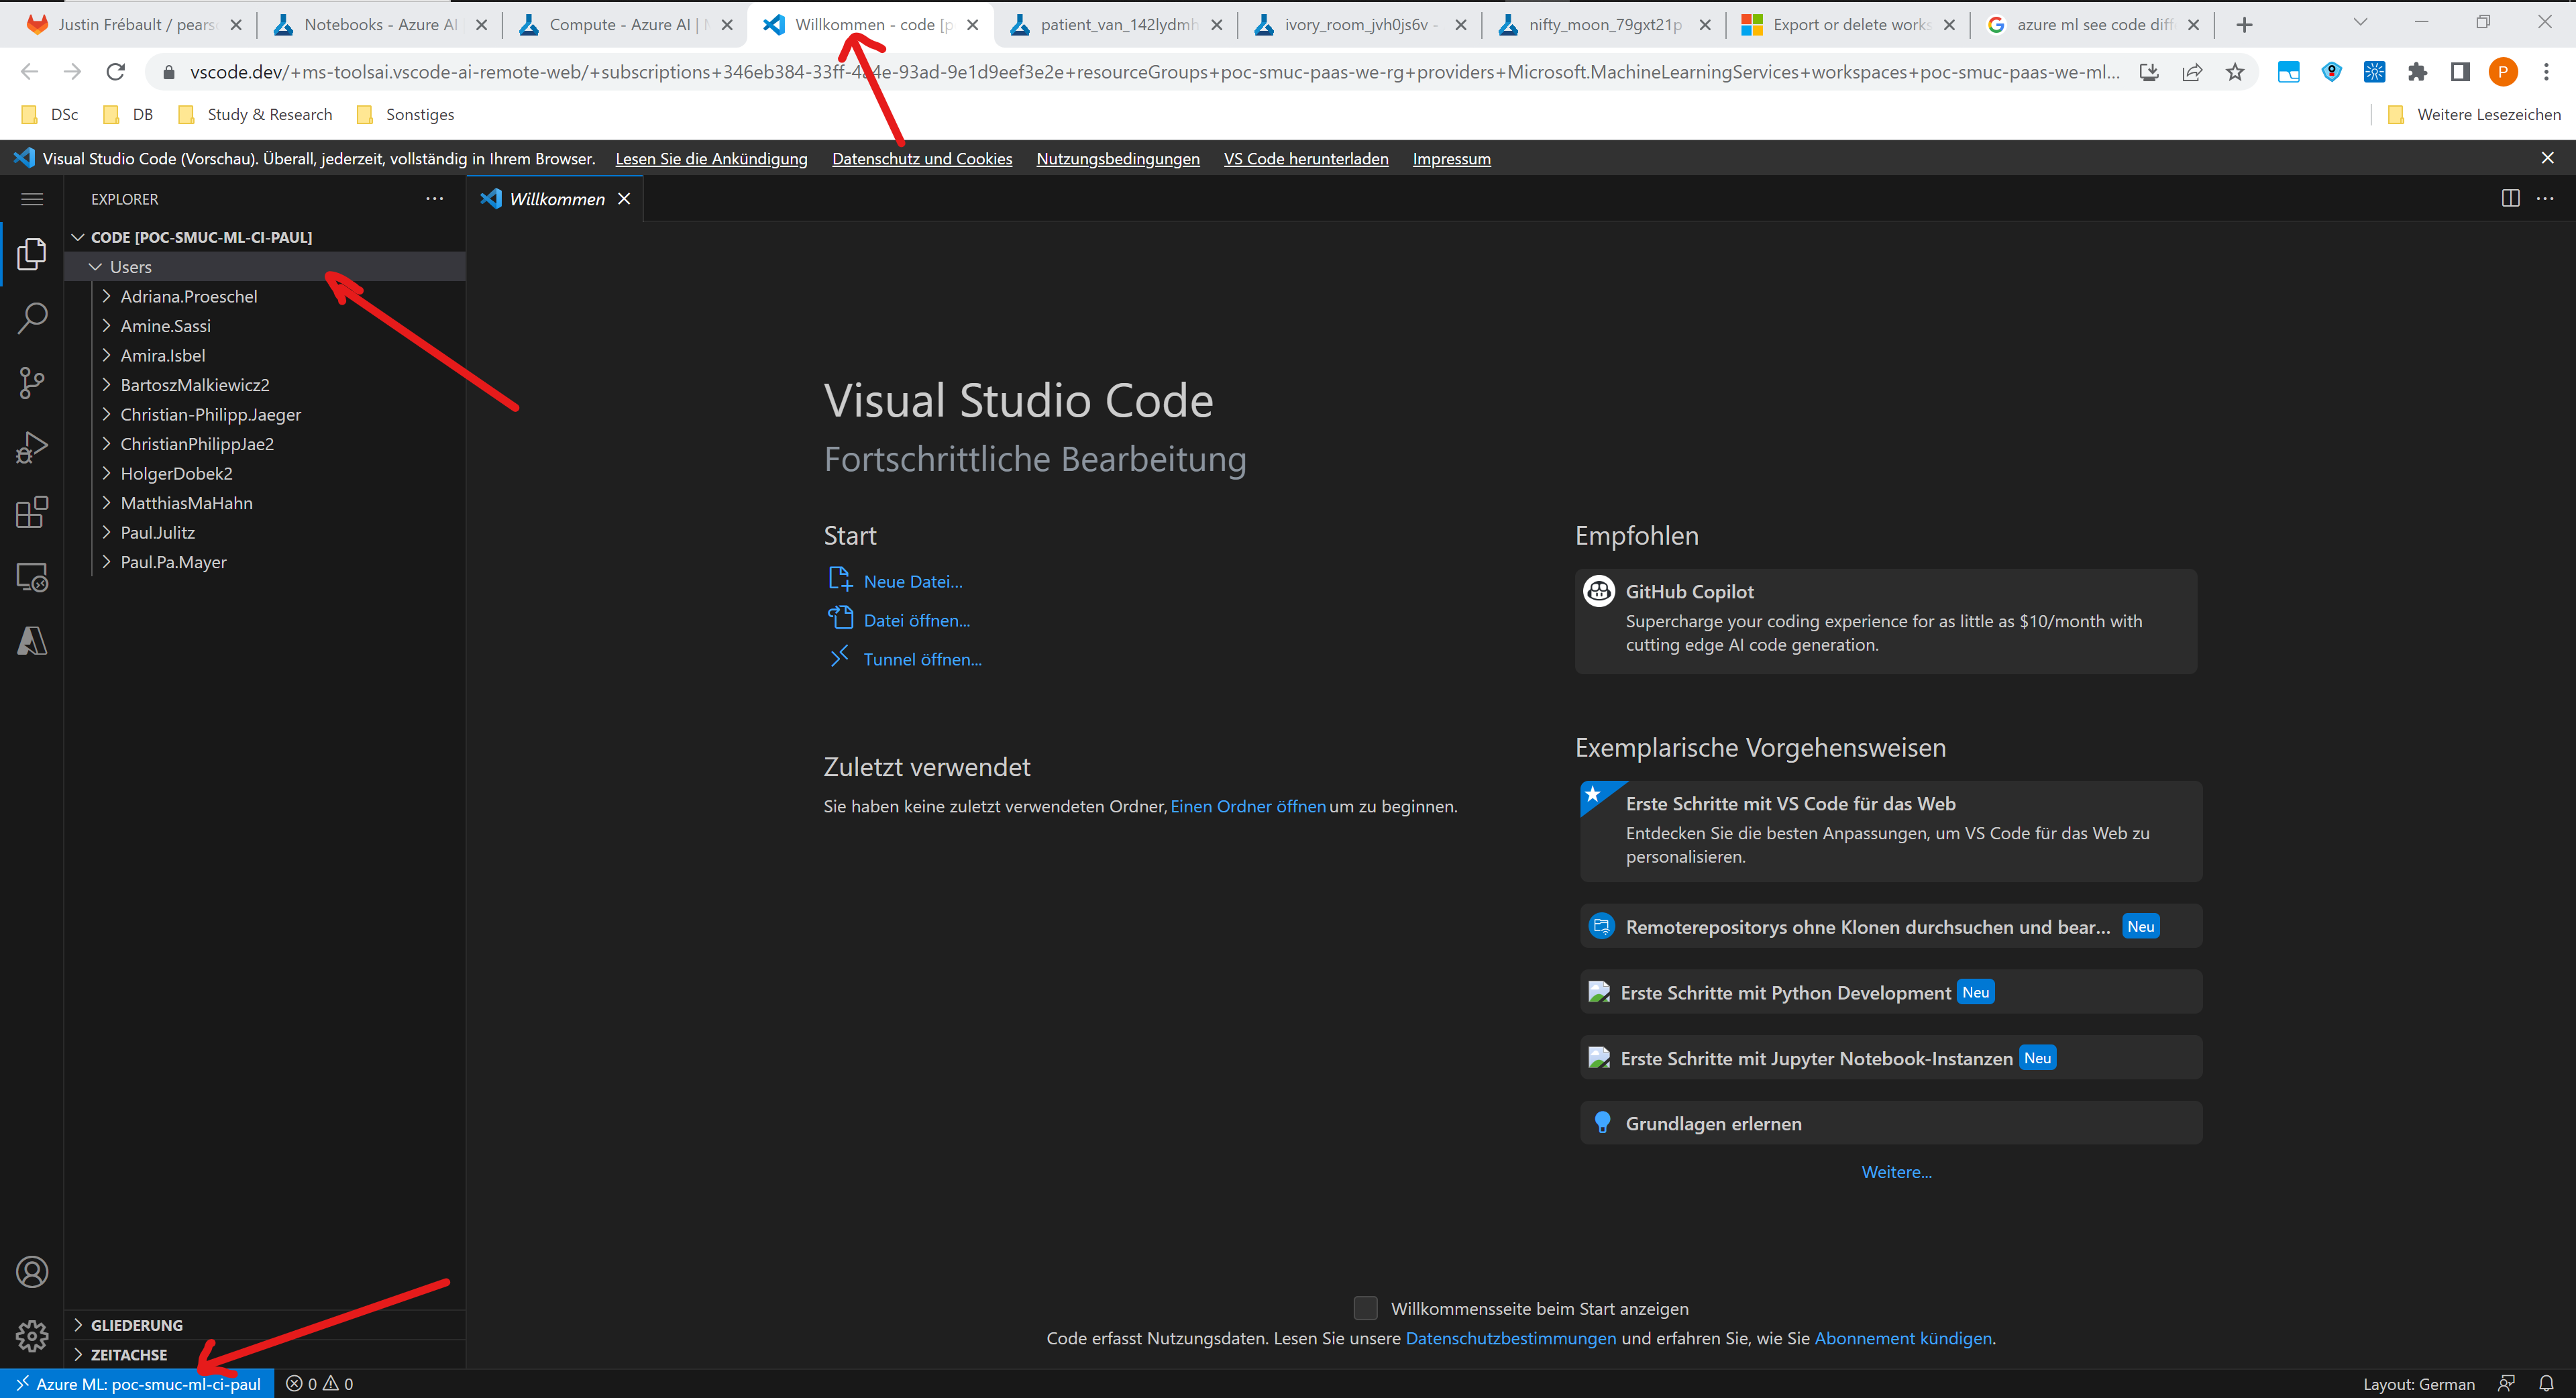
\includegraphics[scale = 0.1]{attachment/chapter_10/Scc049}
	\caption{IDE option: No version controll}
\end{figure}

Either by opening the connection from the compute ressource
 \begin{figure}[H]
 	\centering
 	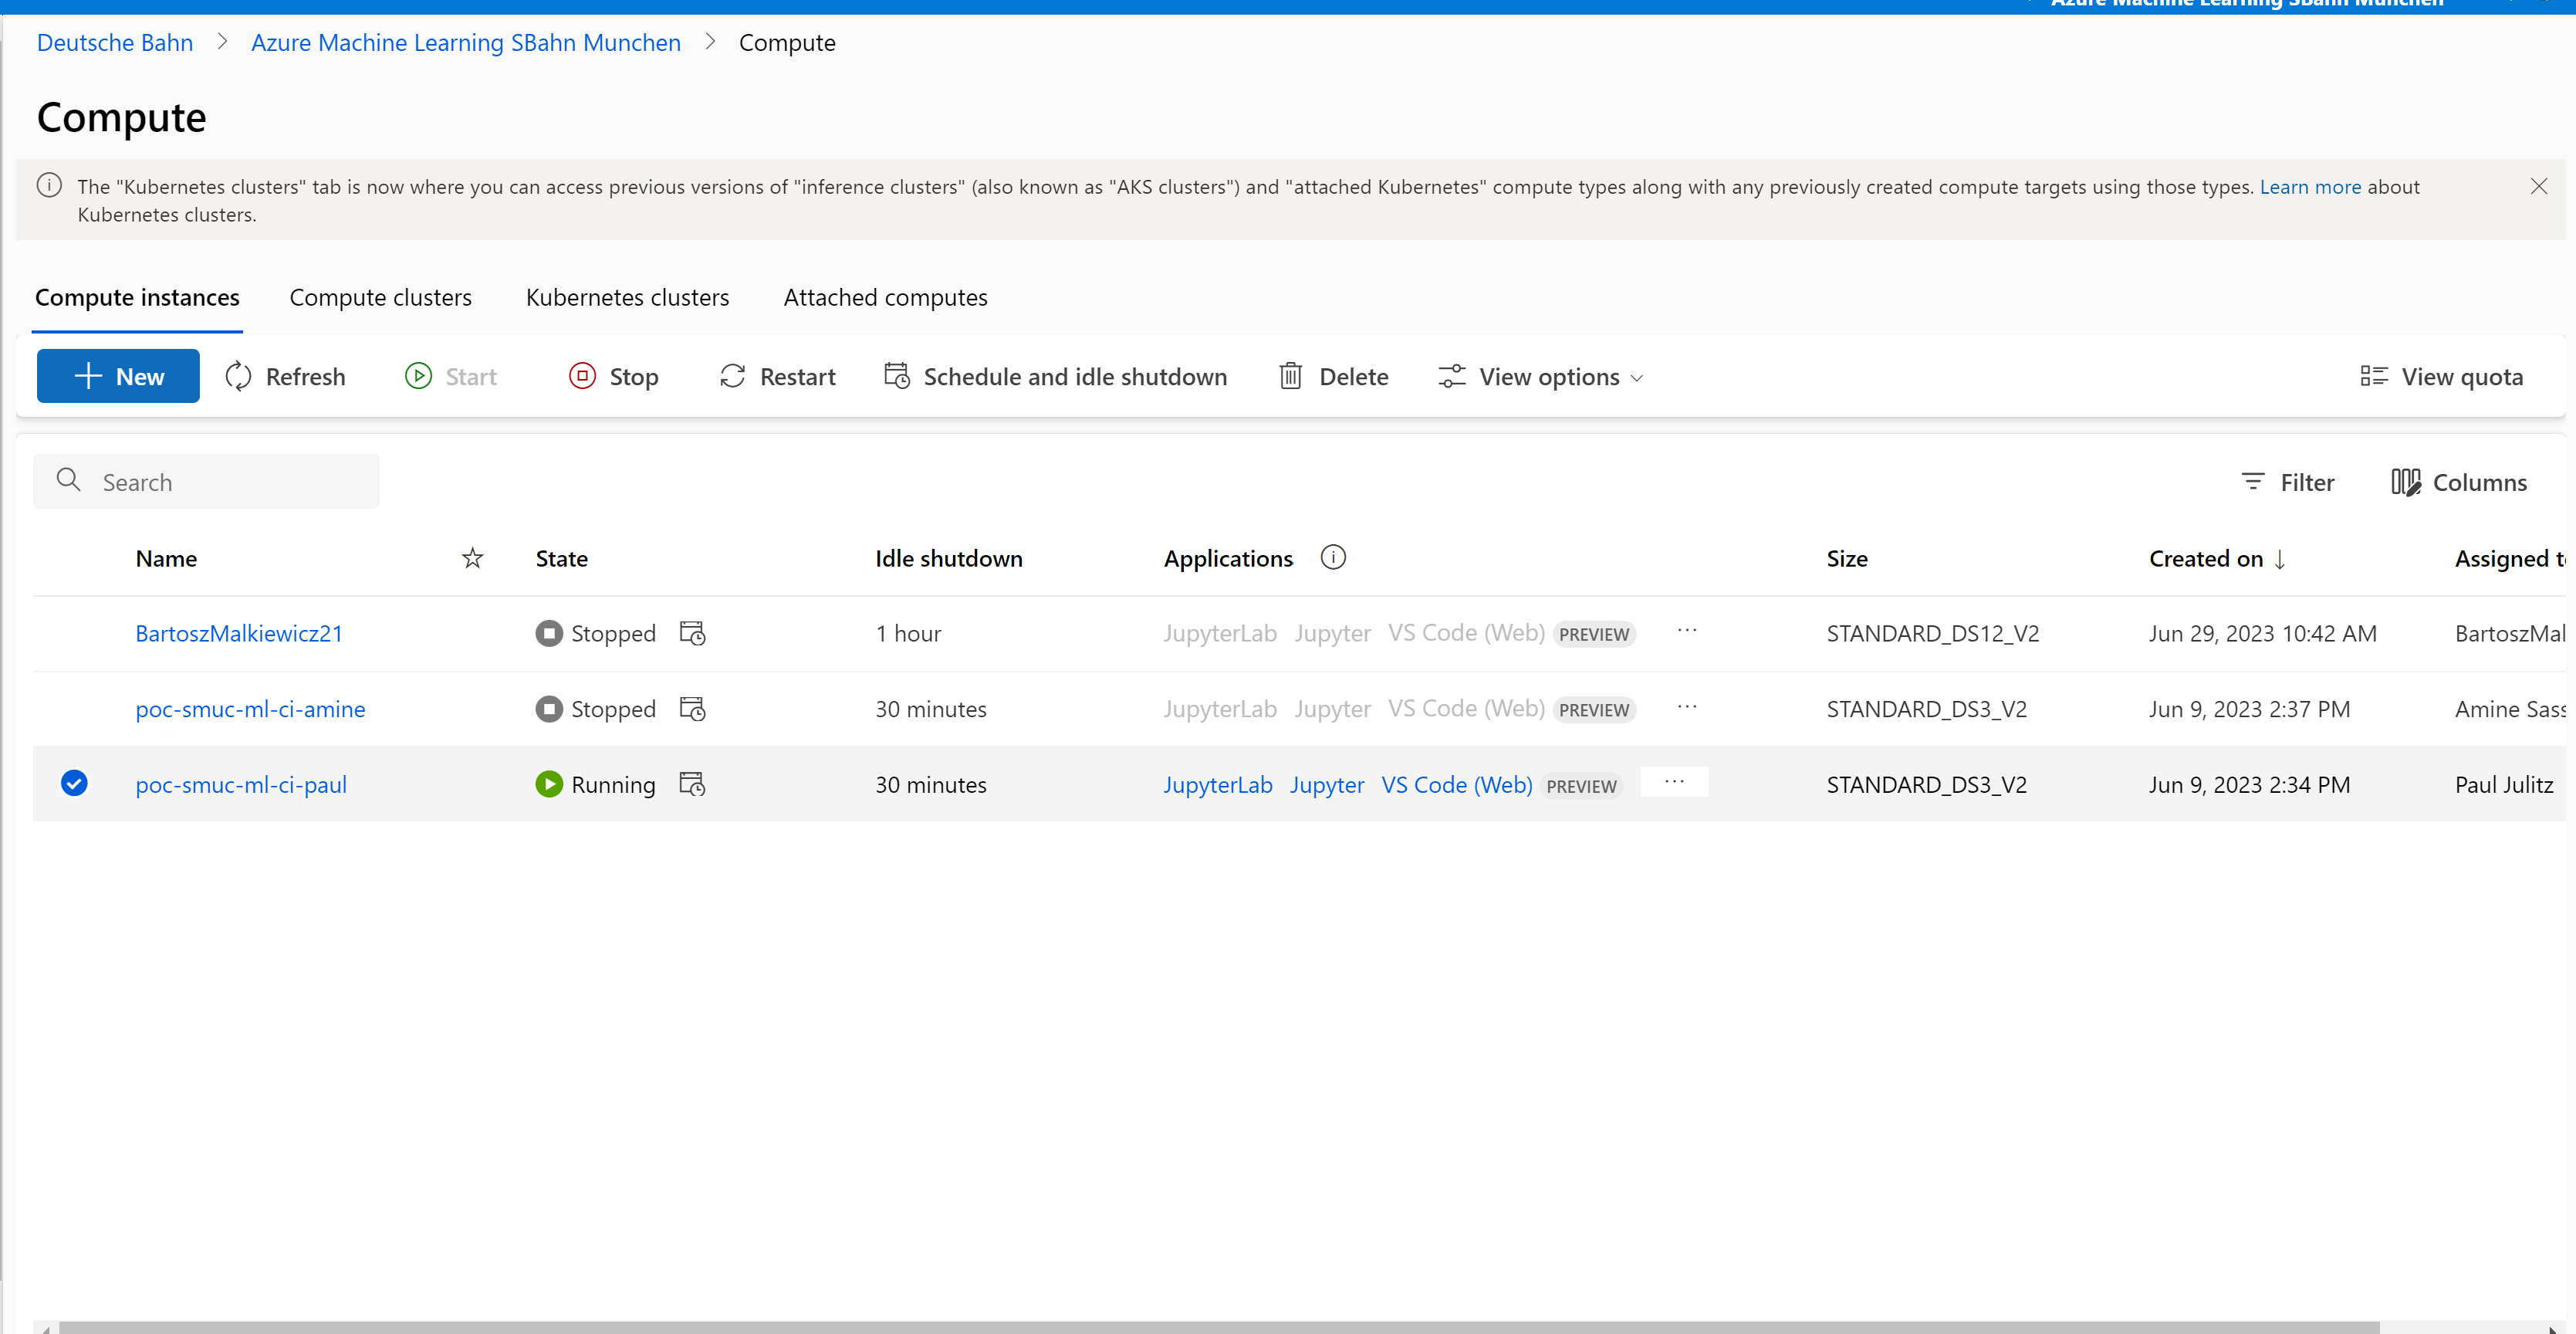
\includegraphics[scale = 0.3]{attachment/chapter_10/Scc046}
 	\caption{Different preview options are available}
 \end{figure}

%TODO: SDK, git clone repo into notebookes
%%% Contexculasiong 
That sound alright, but I think I miss spelled it.
-————
contextualise
contextualise
contextualise
-————
Thinking again about the subject I just read up on.
%%%%%%%%%%
 
\subsection{Experiments (Jobs)}


Wenn ein Trainingskript durchgeführt wird, kann der Output und die Metriken zu dieser Durchführung getrackt werden. Das gleiche Experiement kann mehrmal mit verschiedenen 
\begin{itemize}
	\item Hyperparameters,
	\item Trainingsdaten und
	\item Einstellungen 
\end{itemize}
durchgeführt werden. 

Im Arbeitsbereich wird jedes Experiment geloggt mit den Ergebnissen. Diese Logs geben eine Auskunft, den Verlauf eines Modells zu beobachten. Die Änderungen zu verfolgen, welche zu einer Verbesserung geführt haben und wann das Model in Produktion genommen wird.




\section{MLOps for Python models using Azure Machine Learning}

\subsection{Steps in the ML Process}
\paragraph{Aim: Seemless working together}

All models - including those that work perfectly, need
\begin{itemize}
	\item retraining 
	\item and monitoring.
\end{itemize}
The Azure ML Platform provids a \gls{CI}/\gls{CD} experience for machine learning workflow. The capabilities \gls{MLOps}.This allows \textit{ML Engineer} and Data Scientist to work more seemless together. One is designing the model and the other is engineering the deployment and optimizsation.

\paragraph{Data Preparation - Dataset Versoning}
This takes most of the time. Cleaning, getting it shape and having better quality. This process is supported by \textit{Versioning of datasets}. This allows to follow the process of the datasets.

\paragraph{Creating a Model - Experimentation}
To create a model many steps have to be made:
\begin{itemize}
	\item Feature selection,
	\item Algorithmen selection
	\item Fitting the model
	\item Hyperparmeter tuning
\end{itemize}

This process is captured by what is called as \textit{Experimentation}.

\paragraph{Monitoring}
Wenn das Model in der Produktion ist, ist das Monitoring von Relevanz. 

\begin{figure}[H]
	\centering
	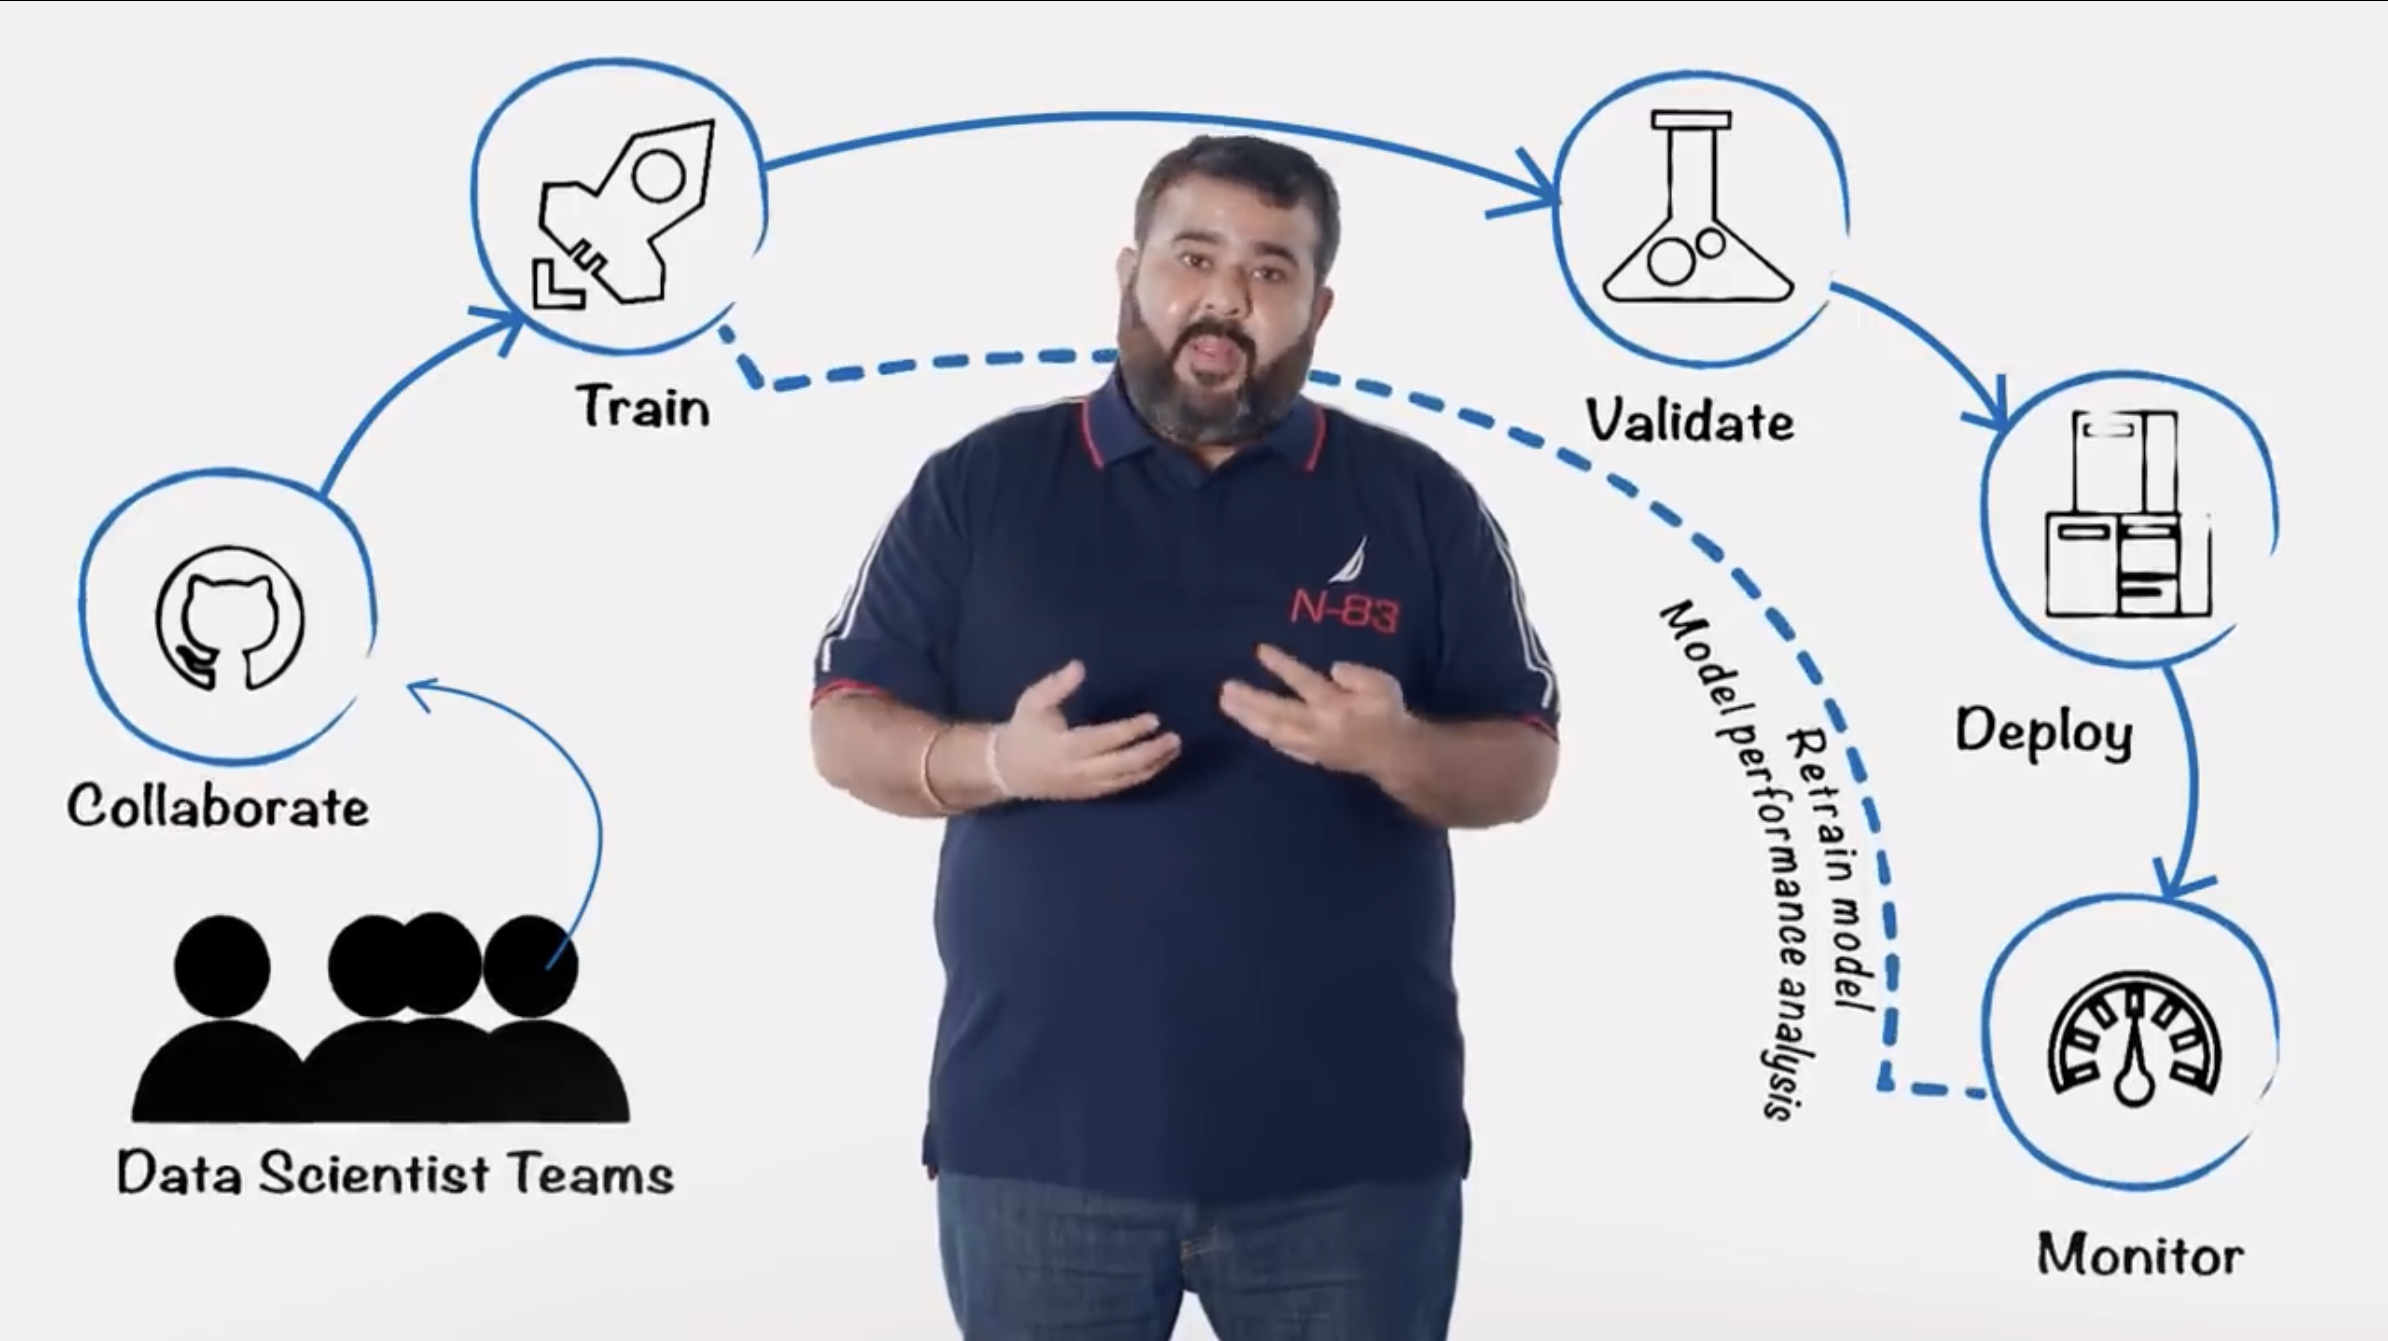
\includegraphics[scale = 0.1]{attachment/chapter_10/Scc025}
	\caption{Monitoring Part in the MLOps Cyclus}
\end{figure}

Es gibt zwei Konzept, welche besonders für den ML Prozess sind:
\begin{description}
	\item[Model Drift] Die geschäftlichen Anforderungen, der Use Case, ändern sich. Das Model muss angepasst werden, weil die Performance sich verschlechtert, weil der Zusammenhang zwischen Input und Output sich geändert haben.
	\begin{figure}[H]
	\centering
	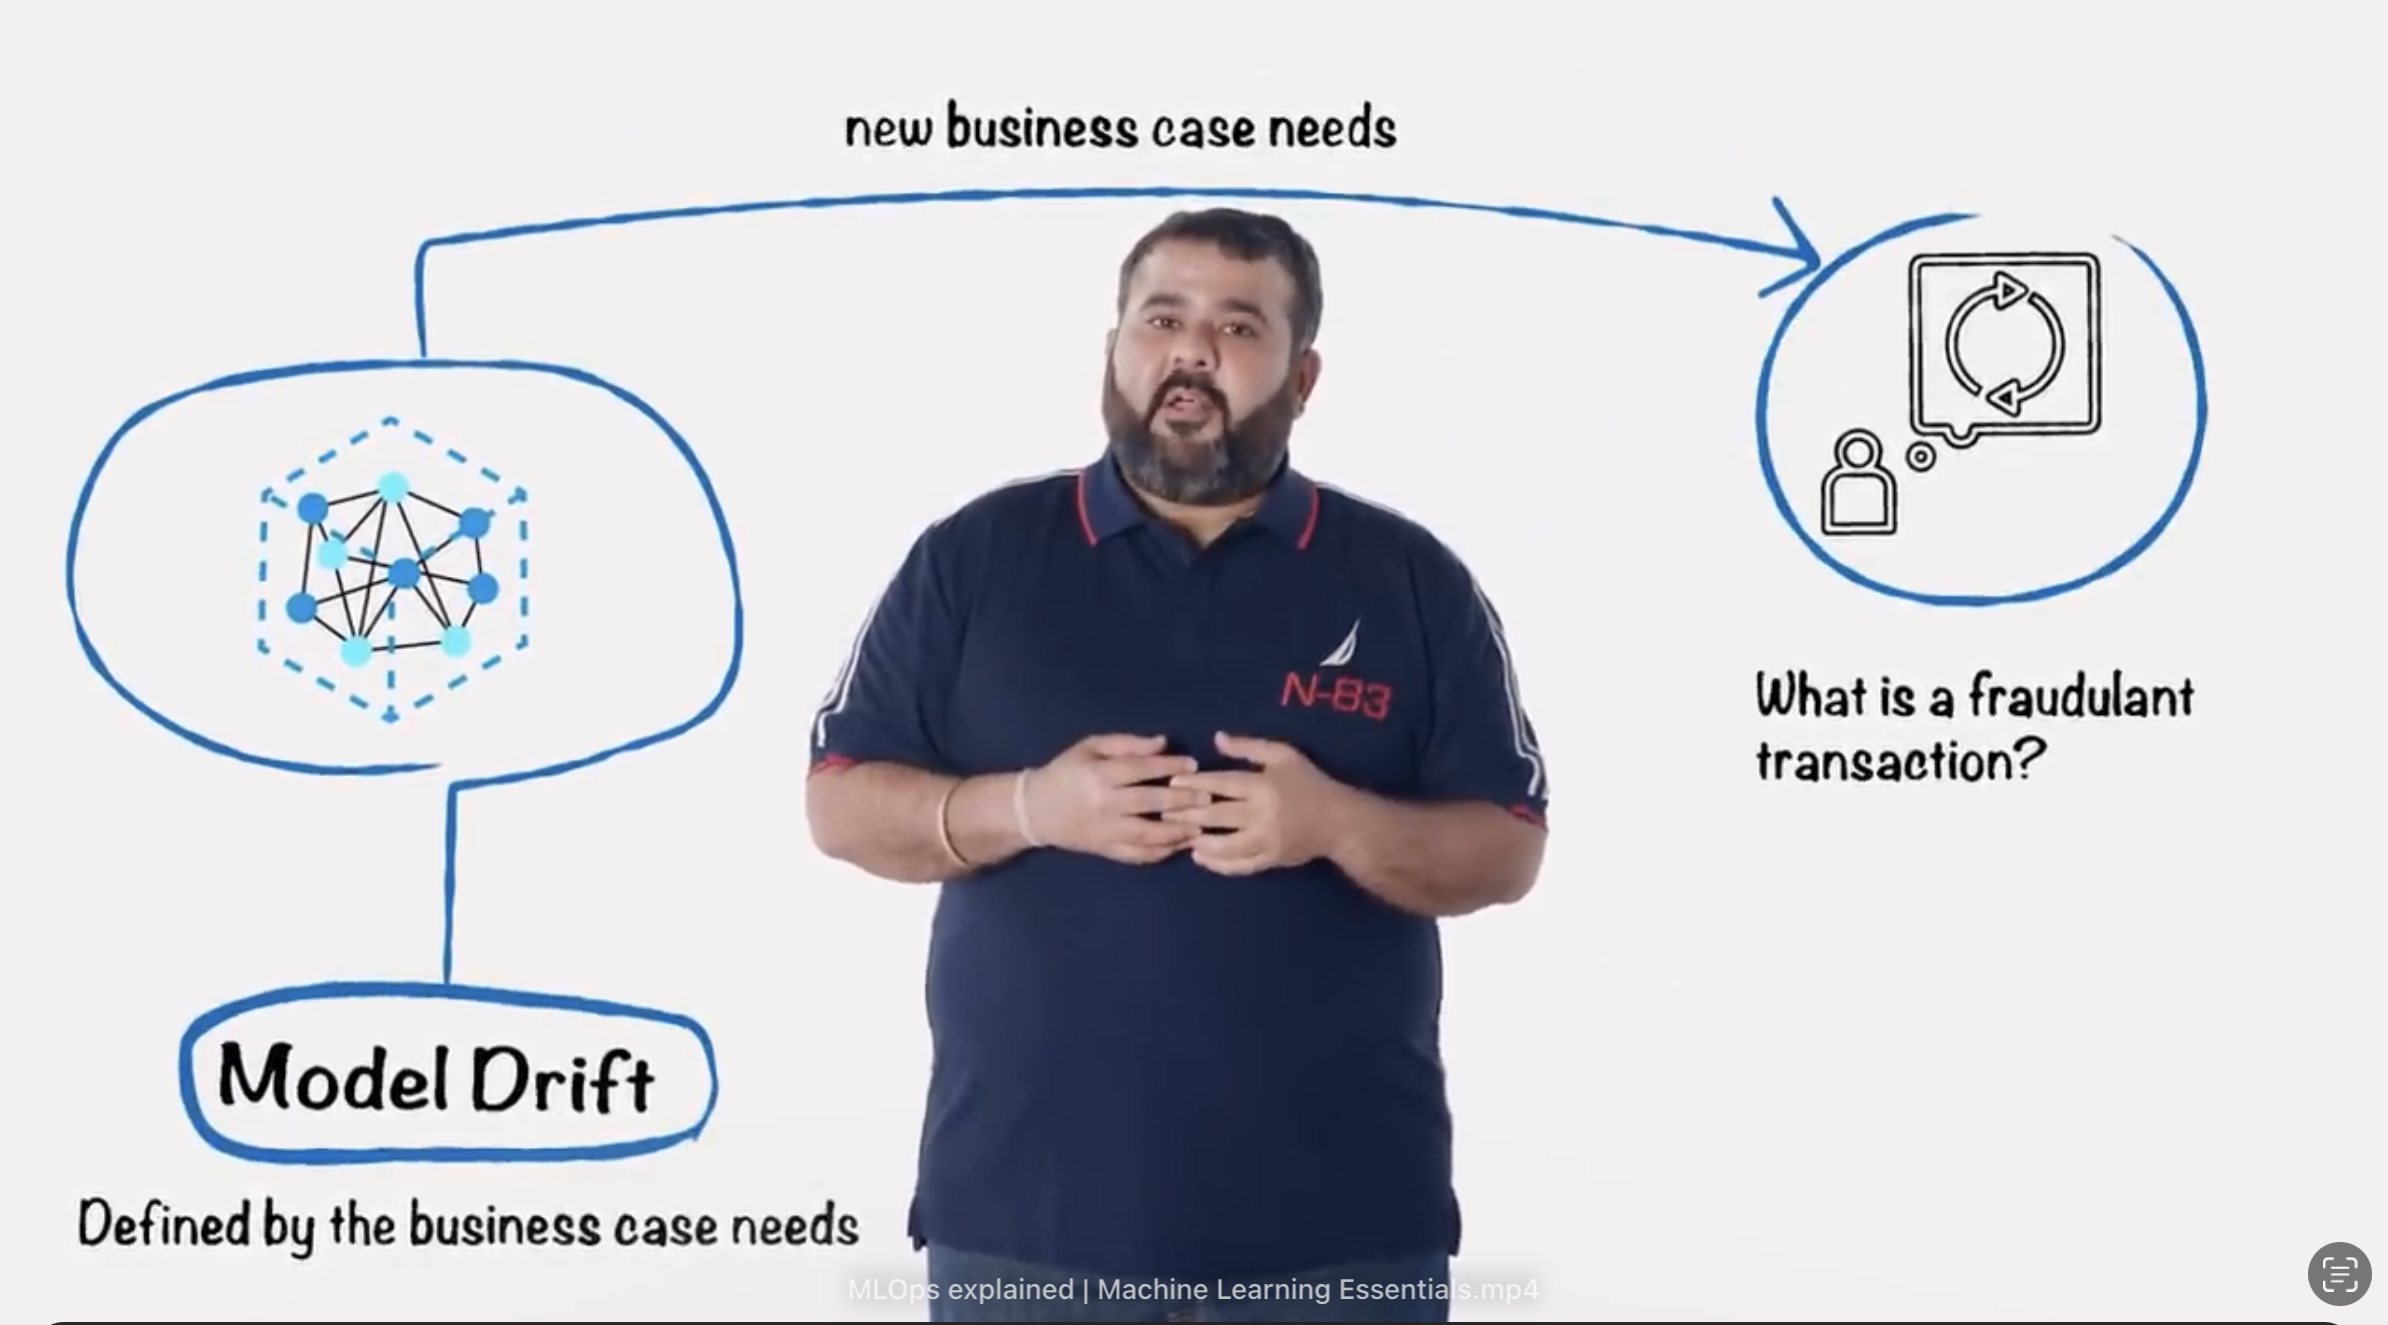
\includegraphics[scale = 0.1]{attachment/chapter_10/Scc027}
	\caption{Example: Different Buisnes Definitions}
\end{figure}
	\item[Data Drift] Zusammenhänge in den Daten ändern sich: Bsp.: Sainalität, Geschlecht. Die Stichprobe entspricht nicht mehr der Verteilung, aus welcher das Model gebildet wurde.
	\begin{figure}[H]
	\centering
	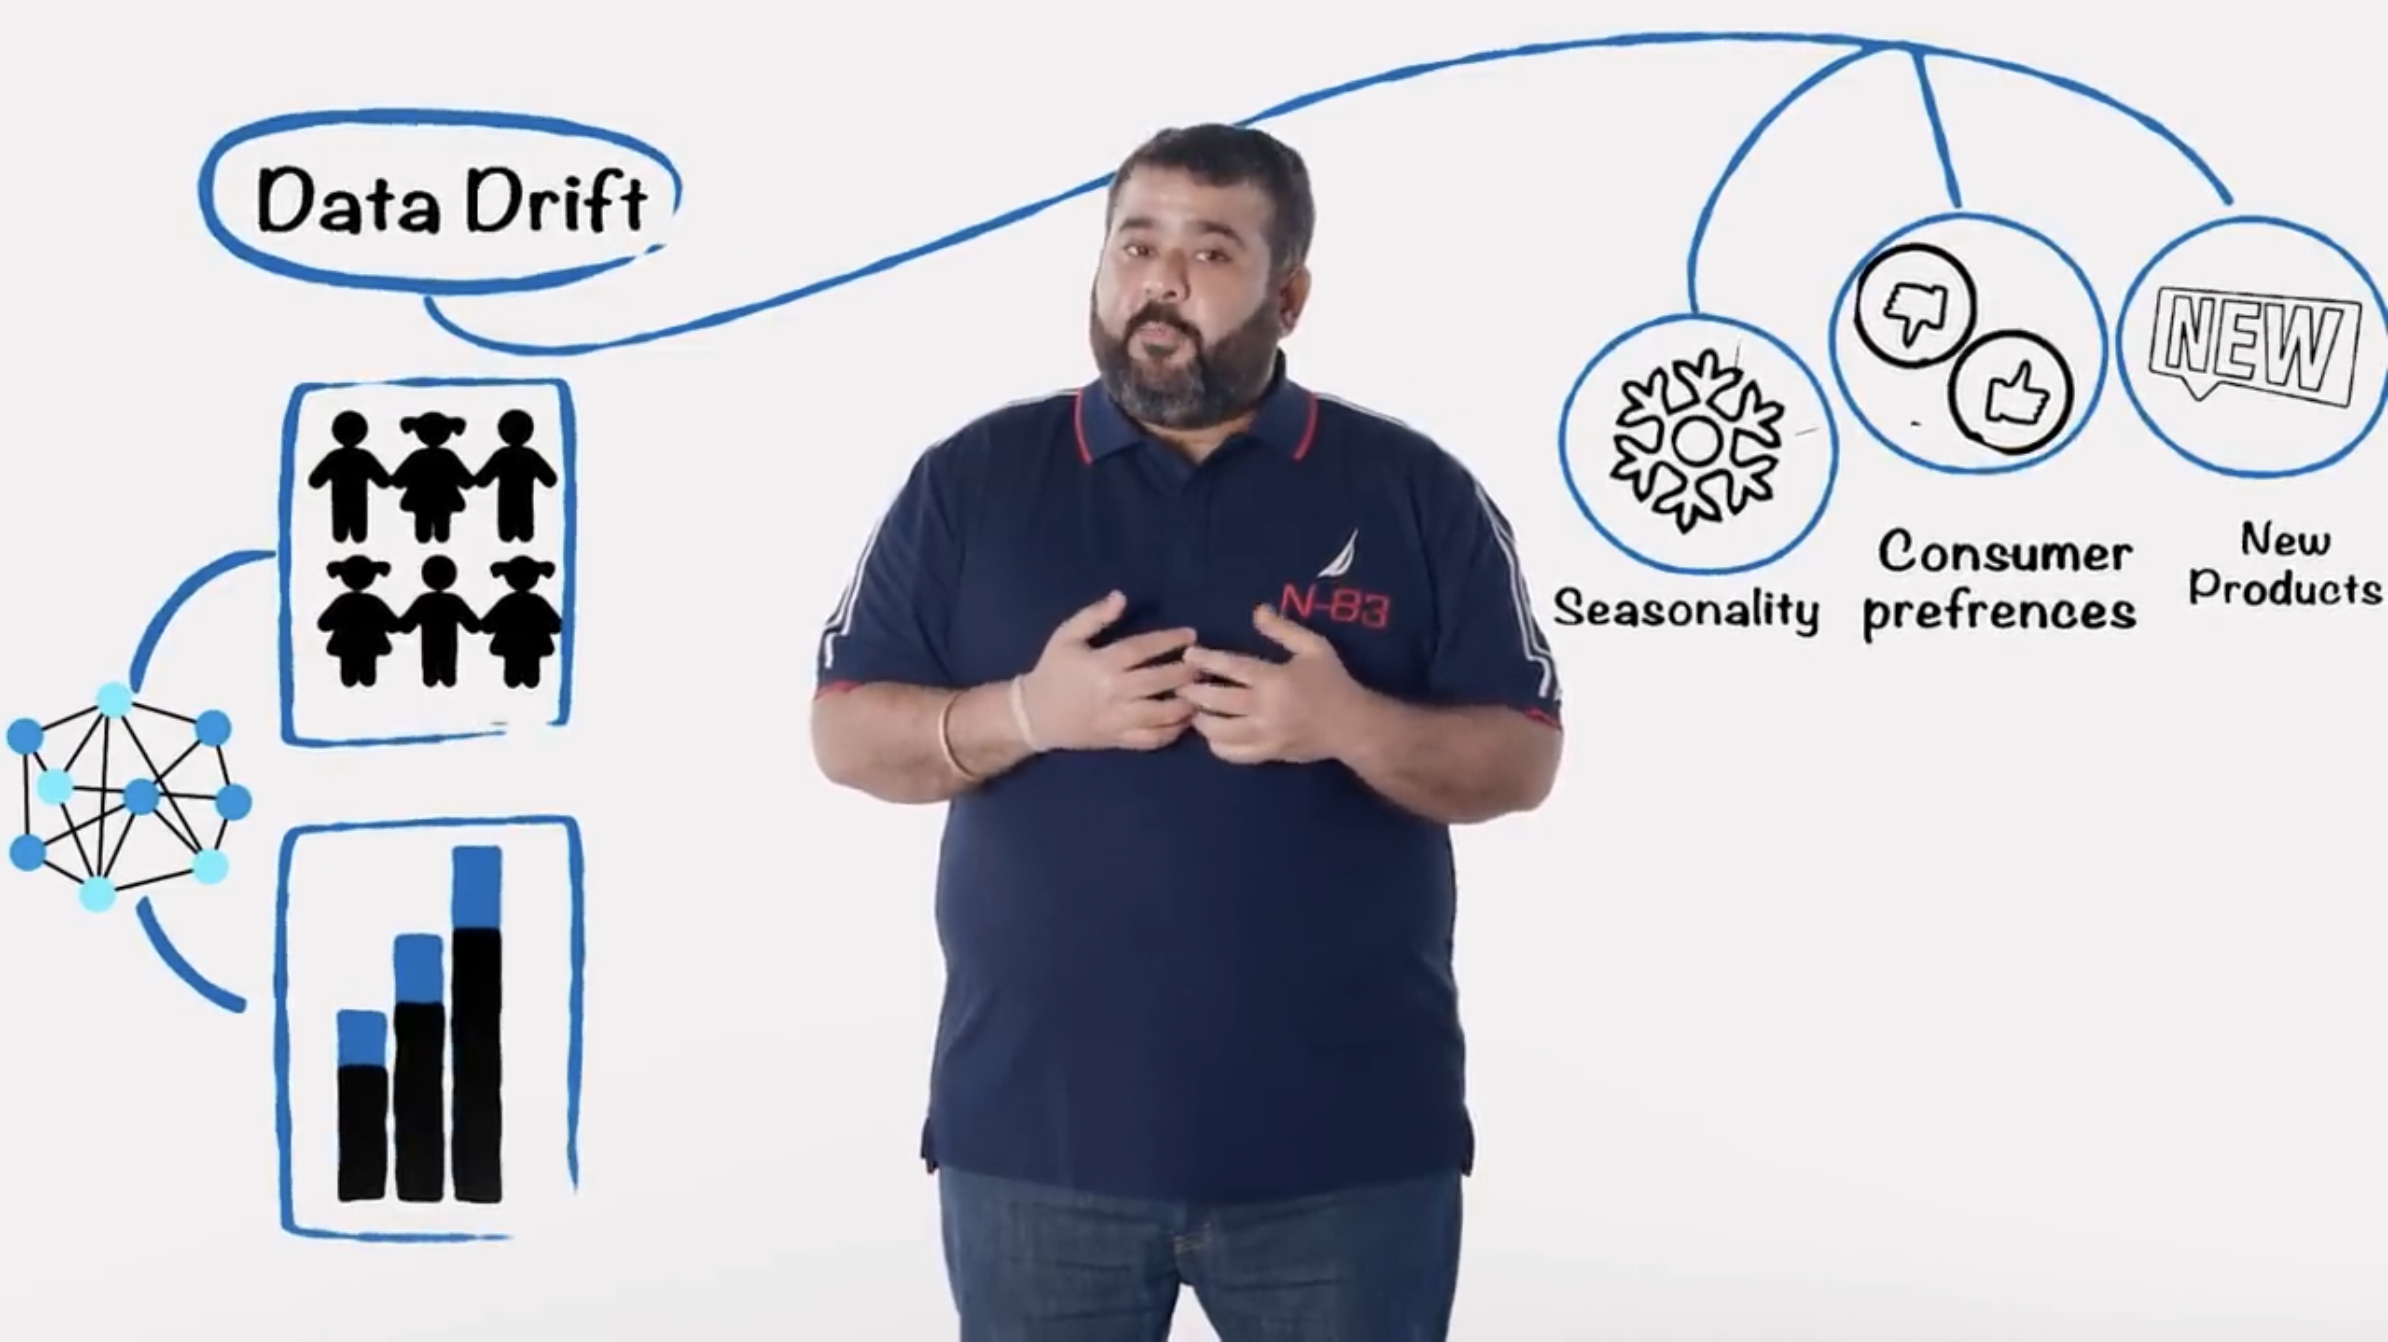
\includegraphics[scale = 0.1]{attachment/chapter_10/Scc026}
	\caption{Examples: Different sample distribution; Seasonality}
\end{figure}
\end{description}




\subsection{CI/CD Process}
\paragraph{Build Pipeline}

With \textit{Azure DevOps} the Testing-Part and setting up required configuration can be done. The \gls{SDK} allows to interact with the components of \textit{Azure ML}. 


\begin{figure}[H]
	\centering
	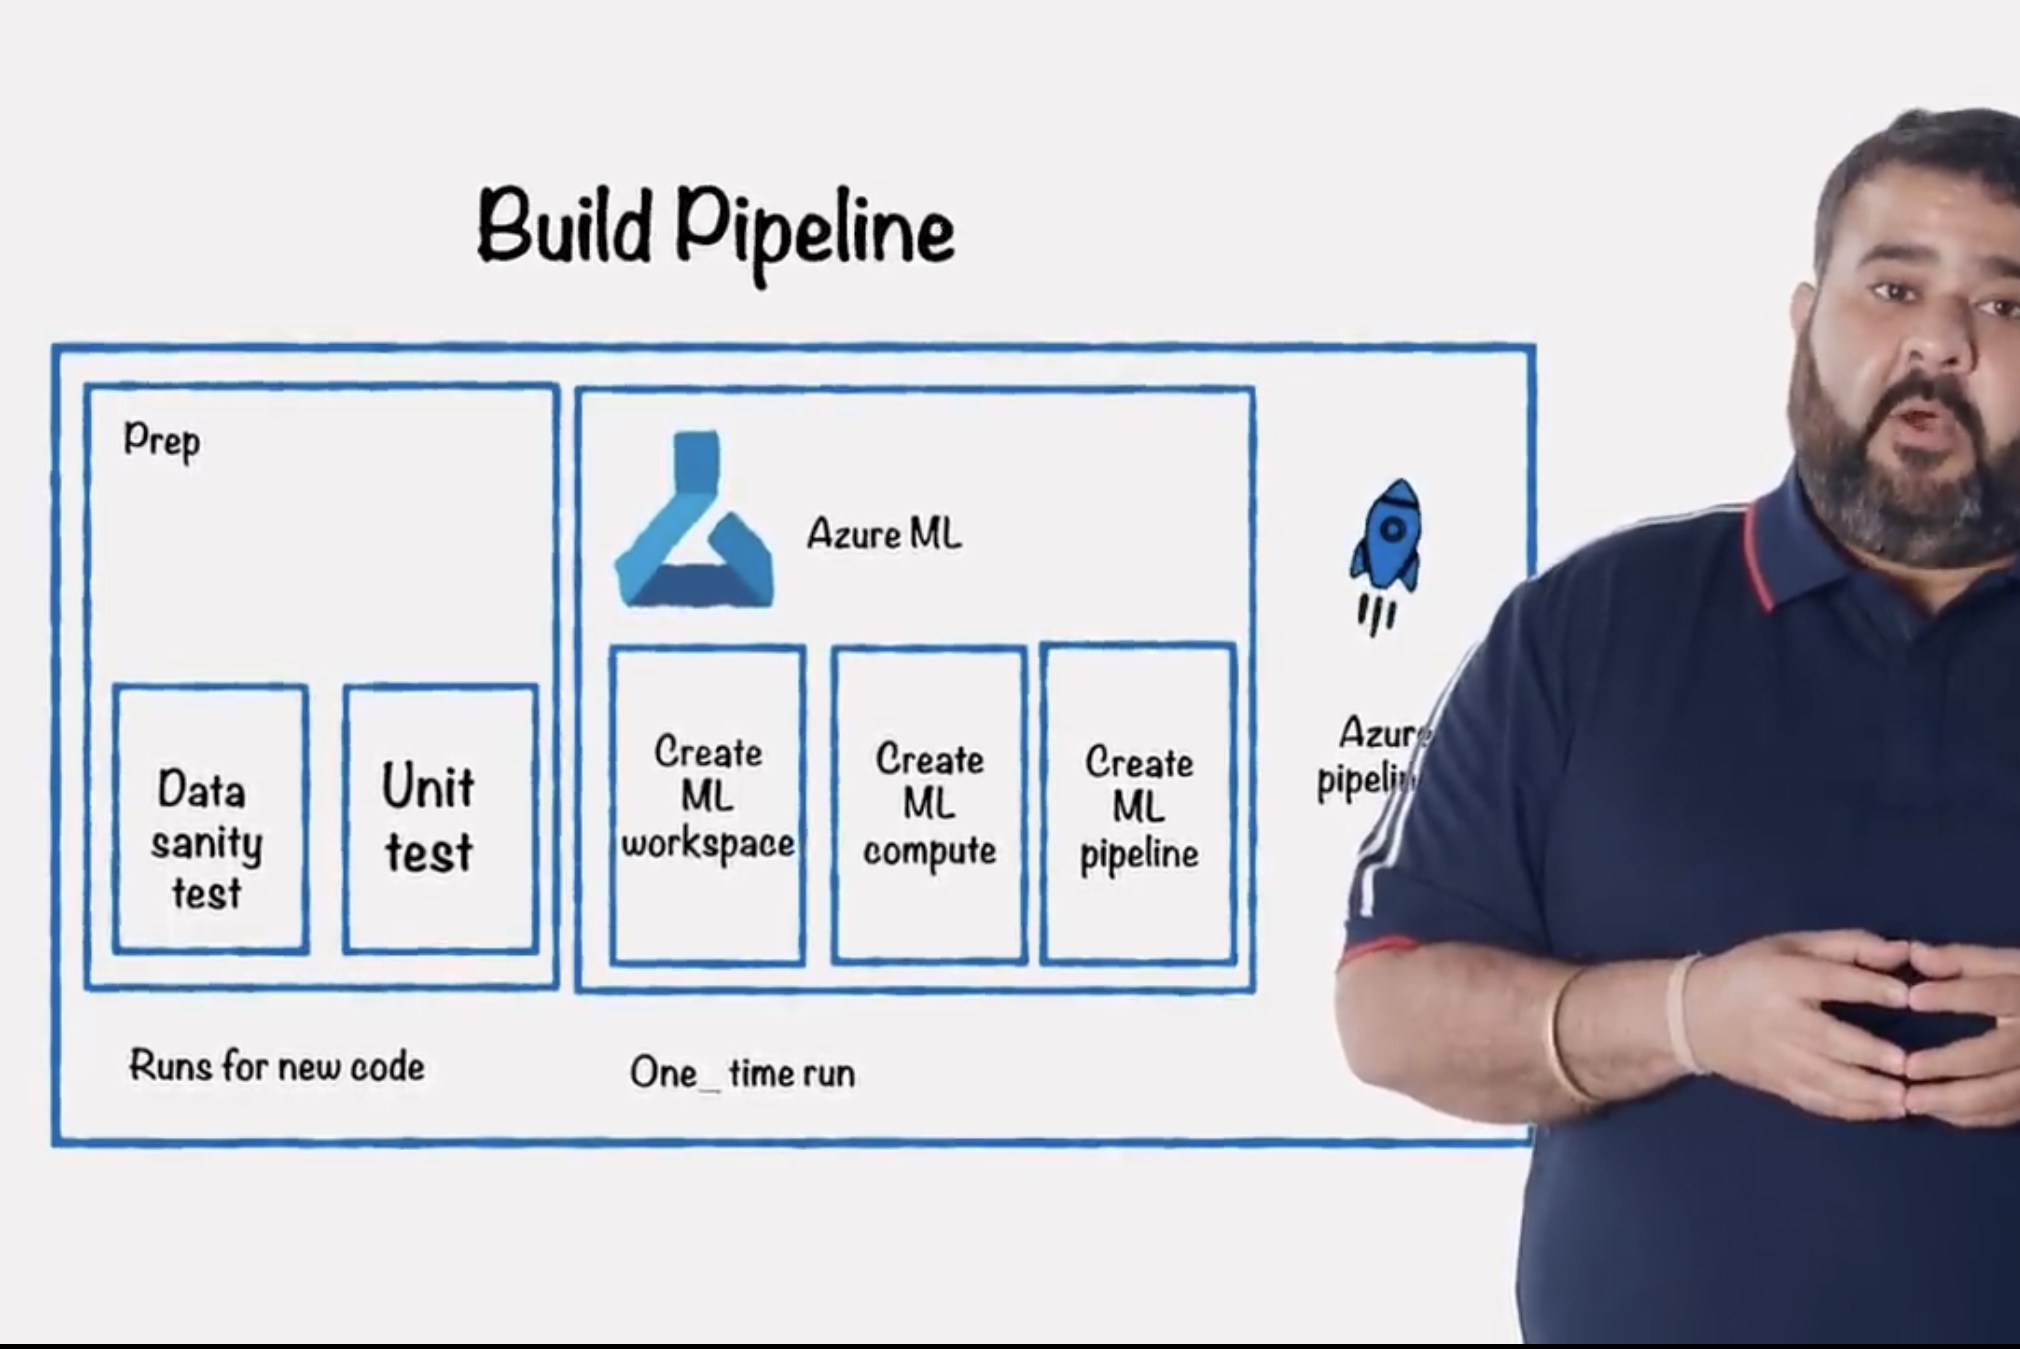
\includegraphics[scale = 0.1]{attachment/chapter_10/Scc020}
	\caption{Once and continuous Build}
\end{figure}

This build pipeline creates once an workspace, compute instances and a pipeline in with a model lives.\\

This architecture is also a setup, for a relativly normal \gls{CI} process. This process works, when you use a repository to change parts in \textit{Azure ML}. \underline{Caution:} The process is different in Azure Synapse Analytics then in Azure ML. In Azure ML the \gls{SDK} gives you a way to interact with the components.

\begin{figure}[H]
	\centering
	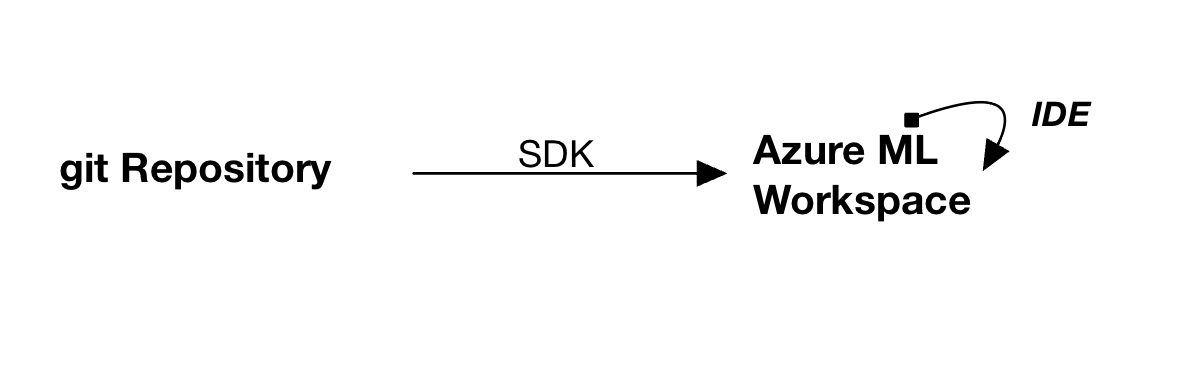
\includegraphics[scale = 0.3]{attachment/chapter_10/Scc021}
	\caption{Interaction with Azure ML}
\end{figure}

In Synapse the hole template for interacting with the ressources can be changed in the repository or vise versa over the \gls{IDE}.

\begin{figure}[H]
	\centering
	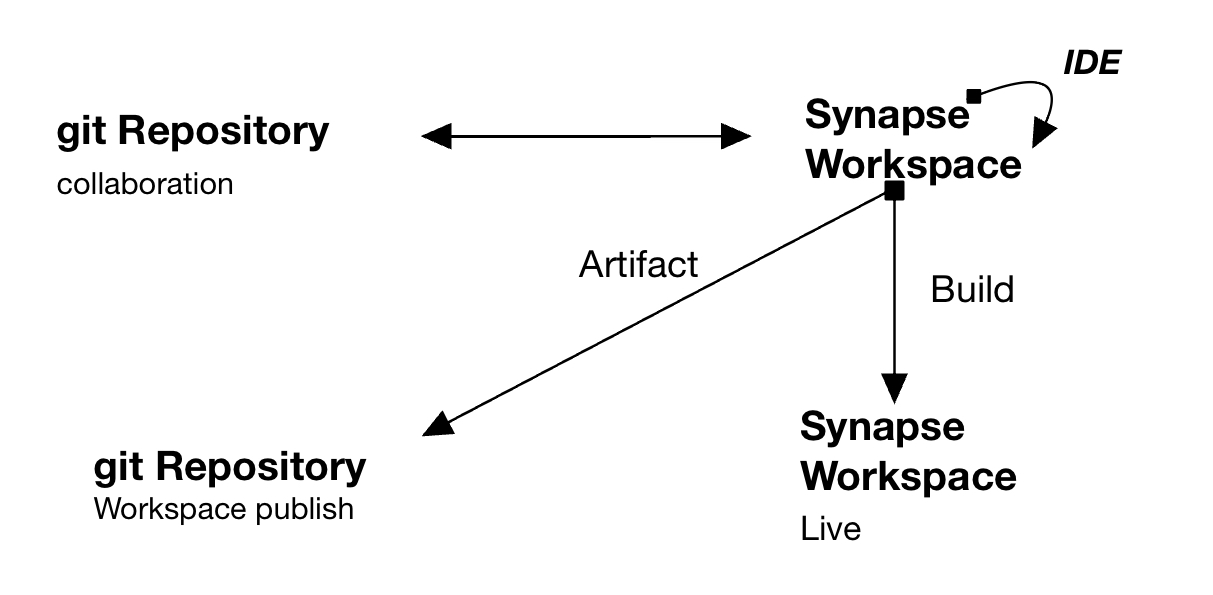
\includegraphics[scale = 0.3]{attachment/chapter_10/Scc022}
	\caption{Interaction with Synapse}
\end{figure}

\paragraph{Retraining Pipeline}

A Azure ML pipeline are reusable workloads. This is can also be use to retrain models. This can be triggered, when a new data is available. With Azure DevOps pipeline can this trigger be identify and the pipeline in Azure Ml be triggered.\\

The retraining steps can include
\begin{itemize}
	\item train on new data
	\item evaluate the new model
	\item and if the efficacy is reached, a new version of the model can be regristered.
\end{itemize}

\begin{figure}[H]
	\centering
	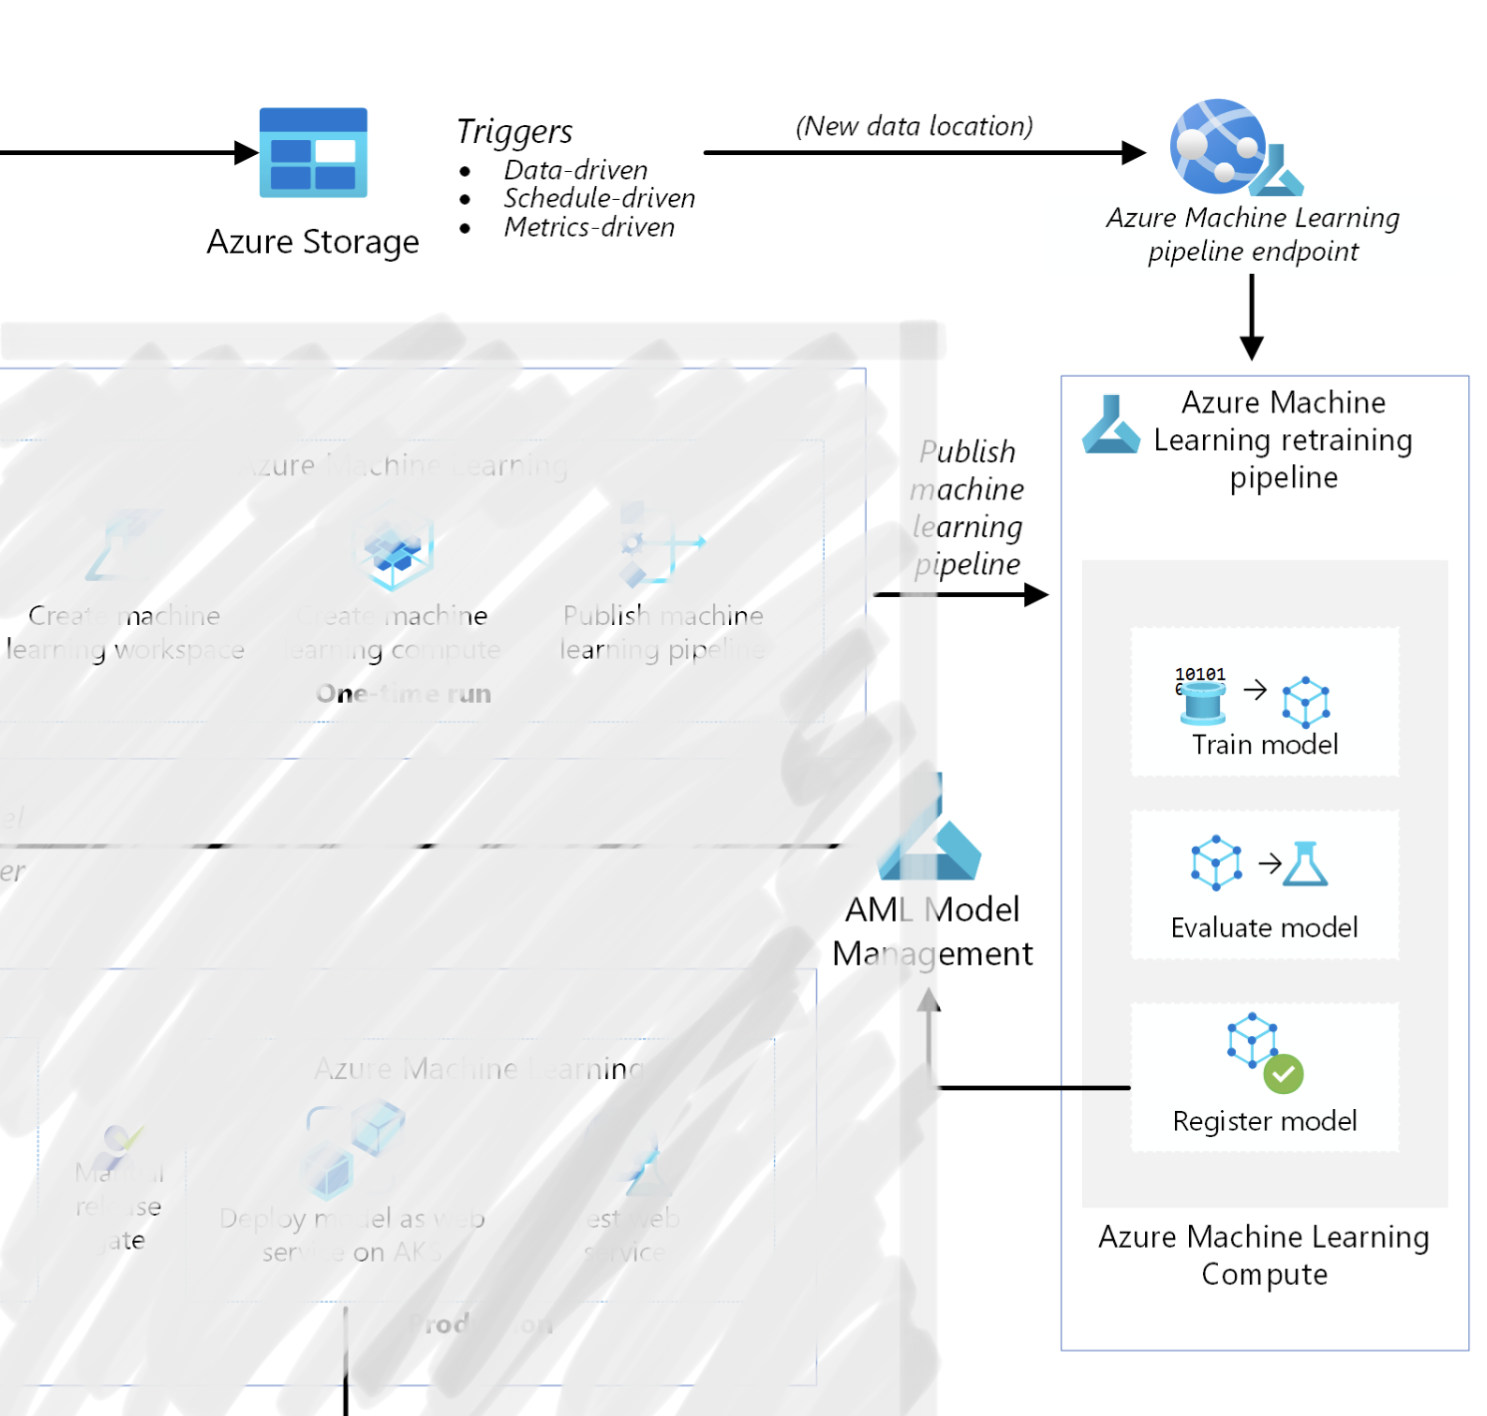
\includegraphics[scale = 0.2]{attachment/chapter_10/Scc023}
	\caption{Example Retraining Pipeline}
\end{figure}

\paragraph{Release Pipeline}
With Azure DevOps Release Pipeline the model gets
\begin{itemize}
	\item page model to and image image,
	\item deploy it to and web service enpoint. 
\end{itemize}
This can be done combined with \textit{managed endpoints}. The webservice in then hosted on a \gls{ACI} for the \textit{Q and A process}. For production load a \gls{AKS} is normally deployed.

\section{Model Deployment and Inferencing}

\subsection{Rewrite a model: Crude or inference methode}

It is possible to receive a model (from a data science team) and rewrite it in the language the application or service is written in. This is not always possible and if it is, then a change in logic of the model will lead to a change in rewritten model as well. This is not scalable, because every time the model changes, this will lead probably not to a one-to-one change in the application.

\begin{figure}[H]
	\centering
	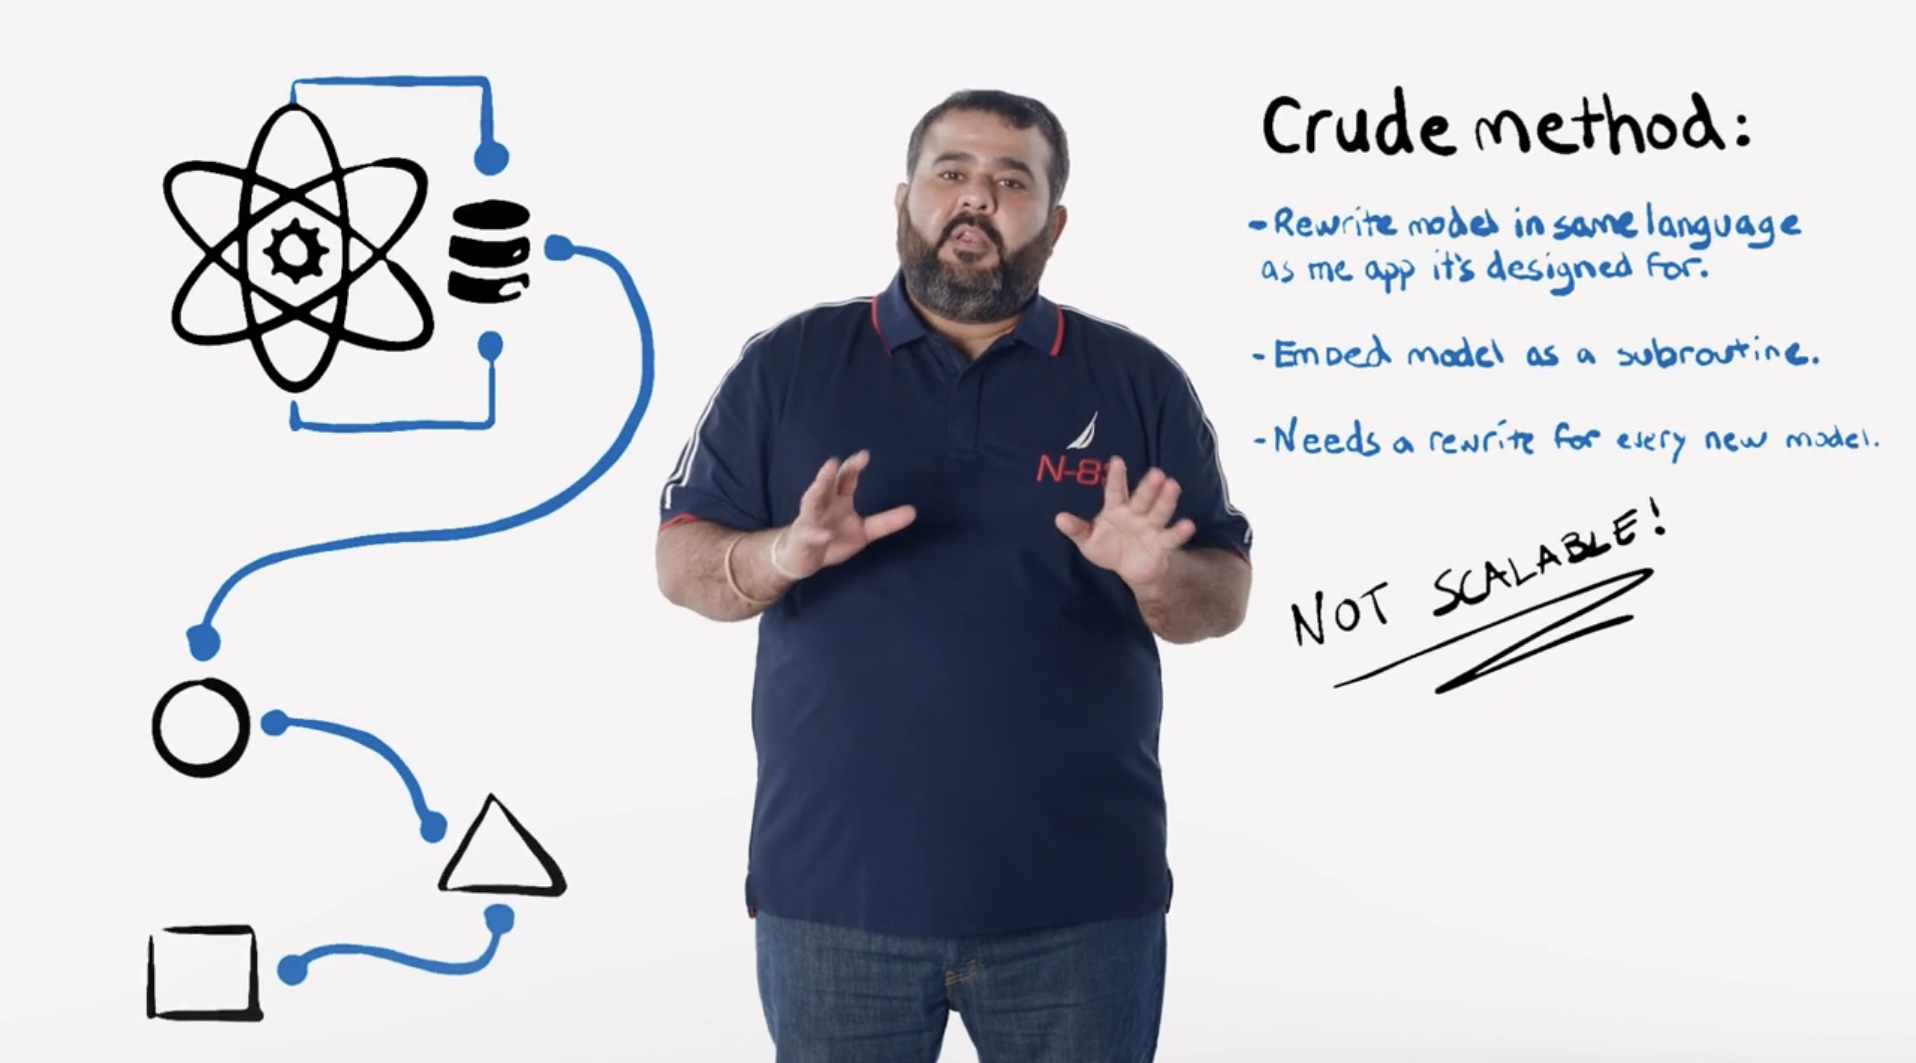
\includegraphics[scale = 0.1]{attachment/chapter_10/Scc009}
\end{figure}

The other solution is to package the model to and hosted as a \textbf{Webservice Endpoint}. This model can then be called when needed. This call is called \textit{Inference call}. This allows
\begin{itemize}
	\item to design a model in the framework and language is most suited, 
	\item and build a microservice architecture for scale. 
\end{itemize}


\begin{figure}[H]
	\centering
	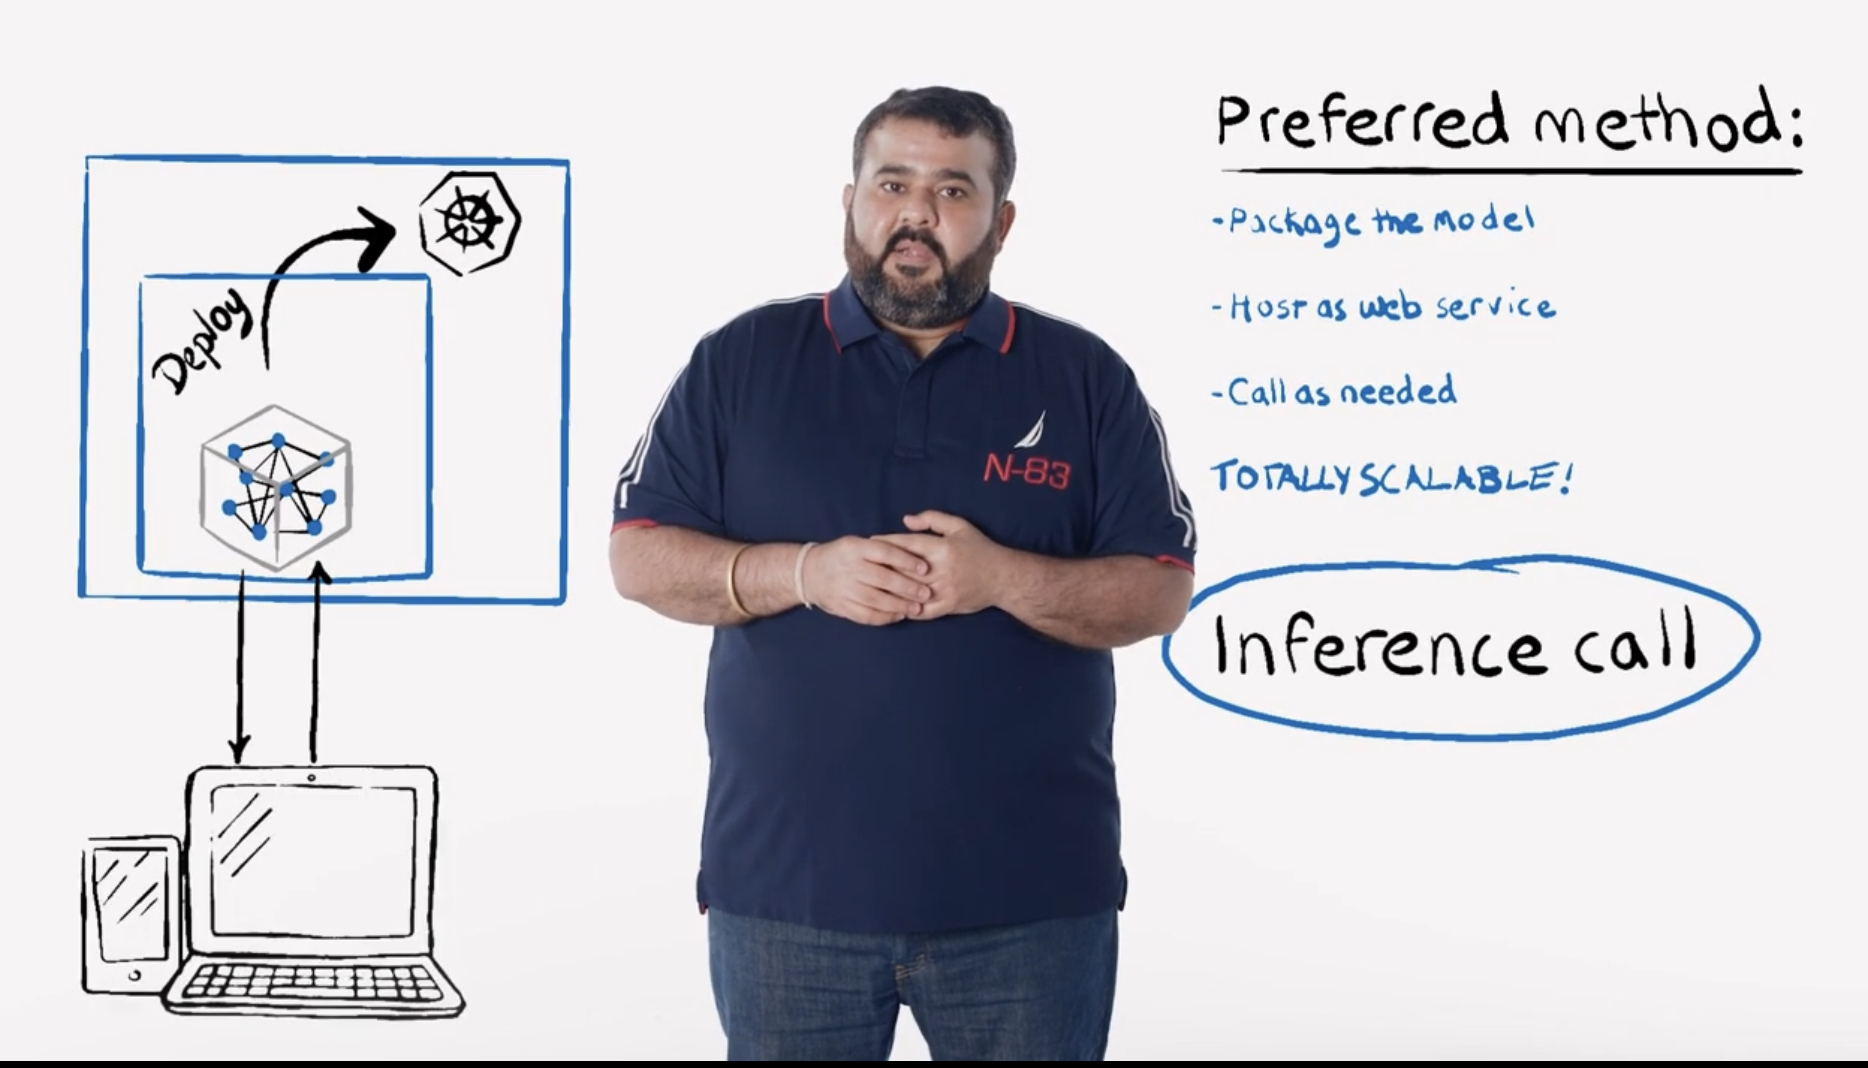
\includegraphics[scale = 0.1]{attachment/chapter_10/Scc010}
\end{figure}





\subsection{Overview Step-by-Step}
The following it structures in a way that, tries to answer the following questing
\begin{itemize}
	\item How to configure the model for the need: Batch, or Realtime
	\item How to set the soring-environment (image) for the model?
	\item How to set the execution-enviornment?
	\item Where to deploy the execution environment?
\end{itemize}
\begin{center}
Config. Model $\rightarrow$ Envir. Soring $\rightarrow$ Envir. Exection $\rightarrow$ Compute Power \\
\end{center}

\subsection{Inference Modes}
\paragraph{Ways to evaluate data send}
When a \textit{inference call} is made, what will happen is, that data is send to the model and the model evaluates the data and returns the evaluated data.
\begin{figure}[H]
	\centering
	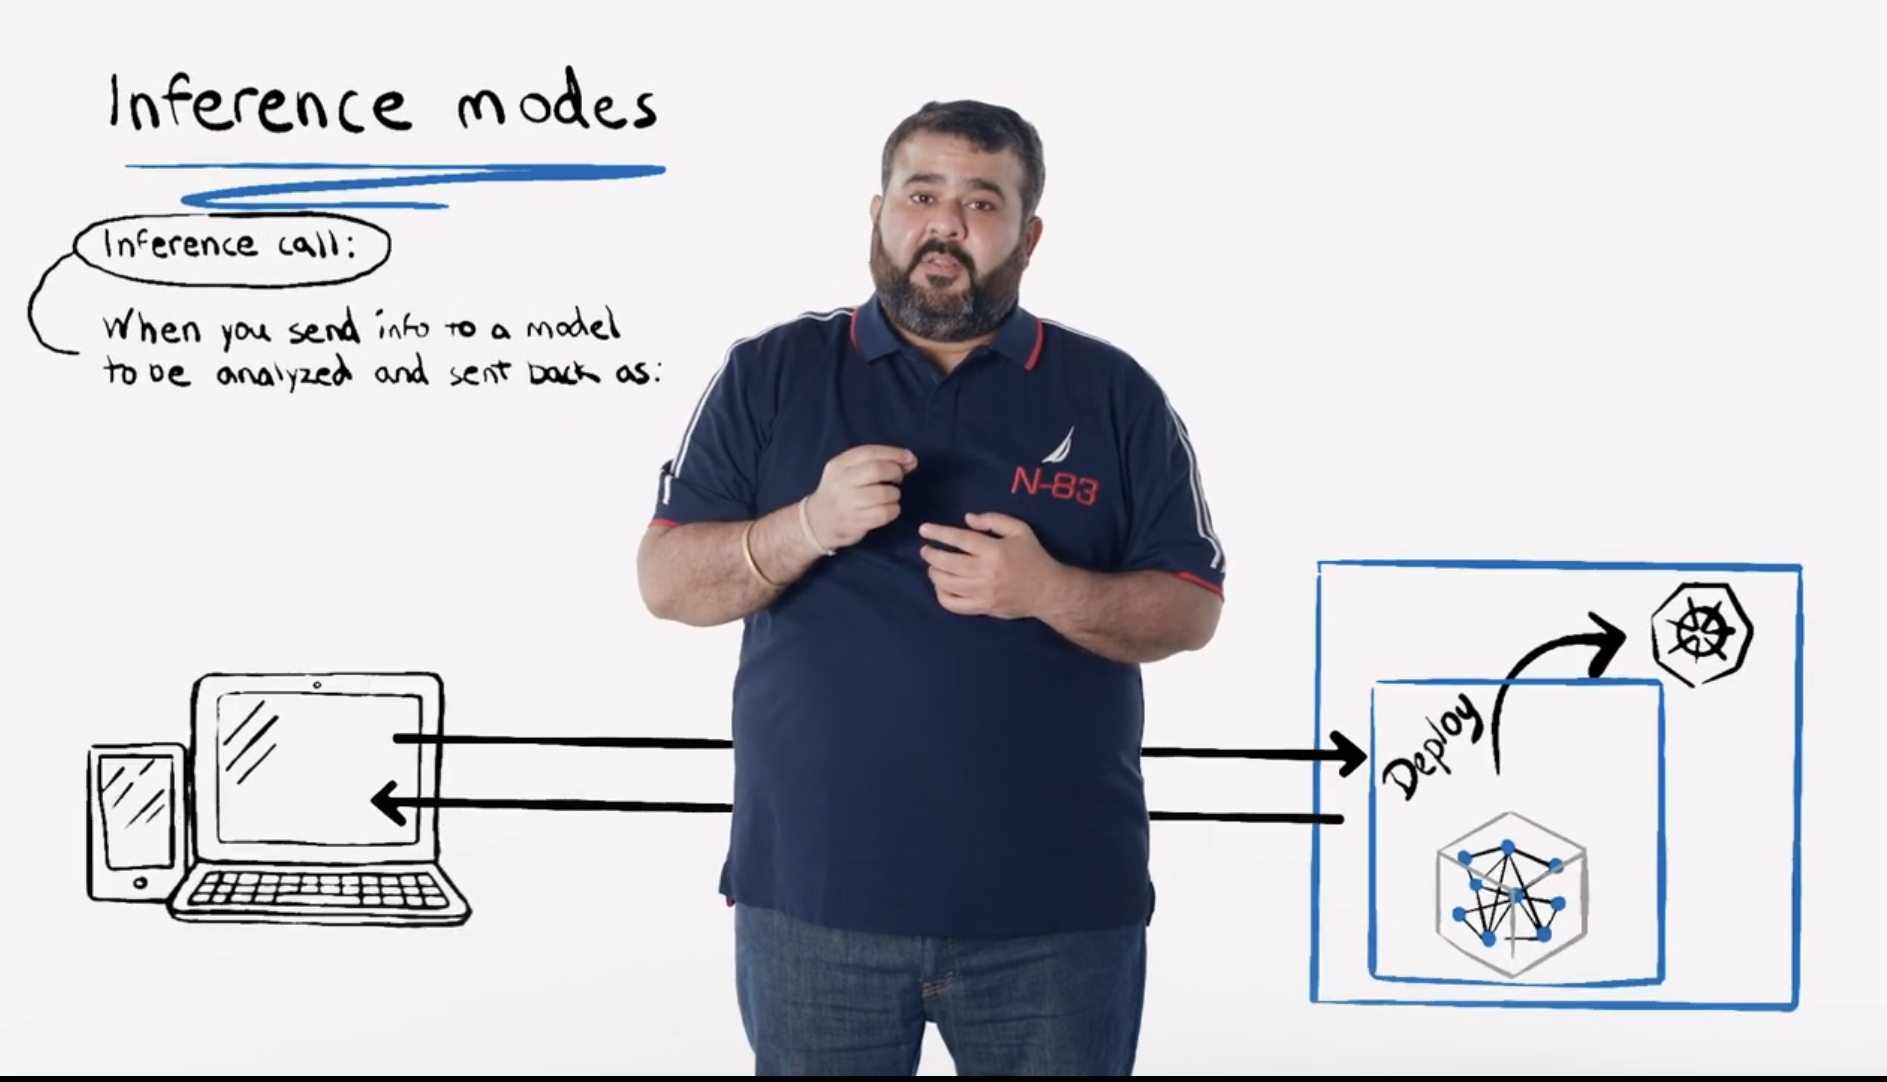
\includegraphics[scale = 0.1]{attachment/chapter_10/Scc011}
	\caption{Inference modes - Making a inference call}
\end{figure}

\paragraph{Realtime-Tupel or Batch Infereance}
There are two ways this is done:
\begin{itemize}
	\item Realtime-inference 
	\item or Batch-inference
\end{itemize}

\begin{figure}[H]
	\centering
	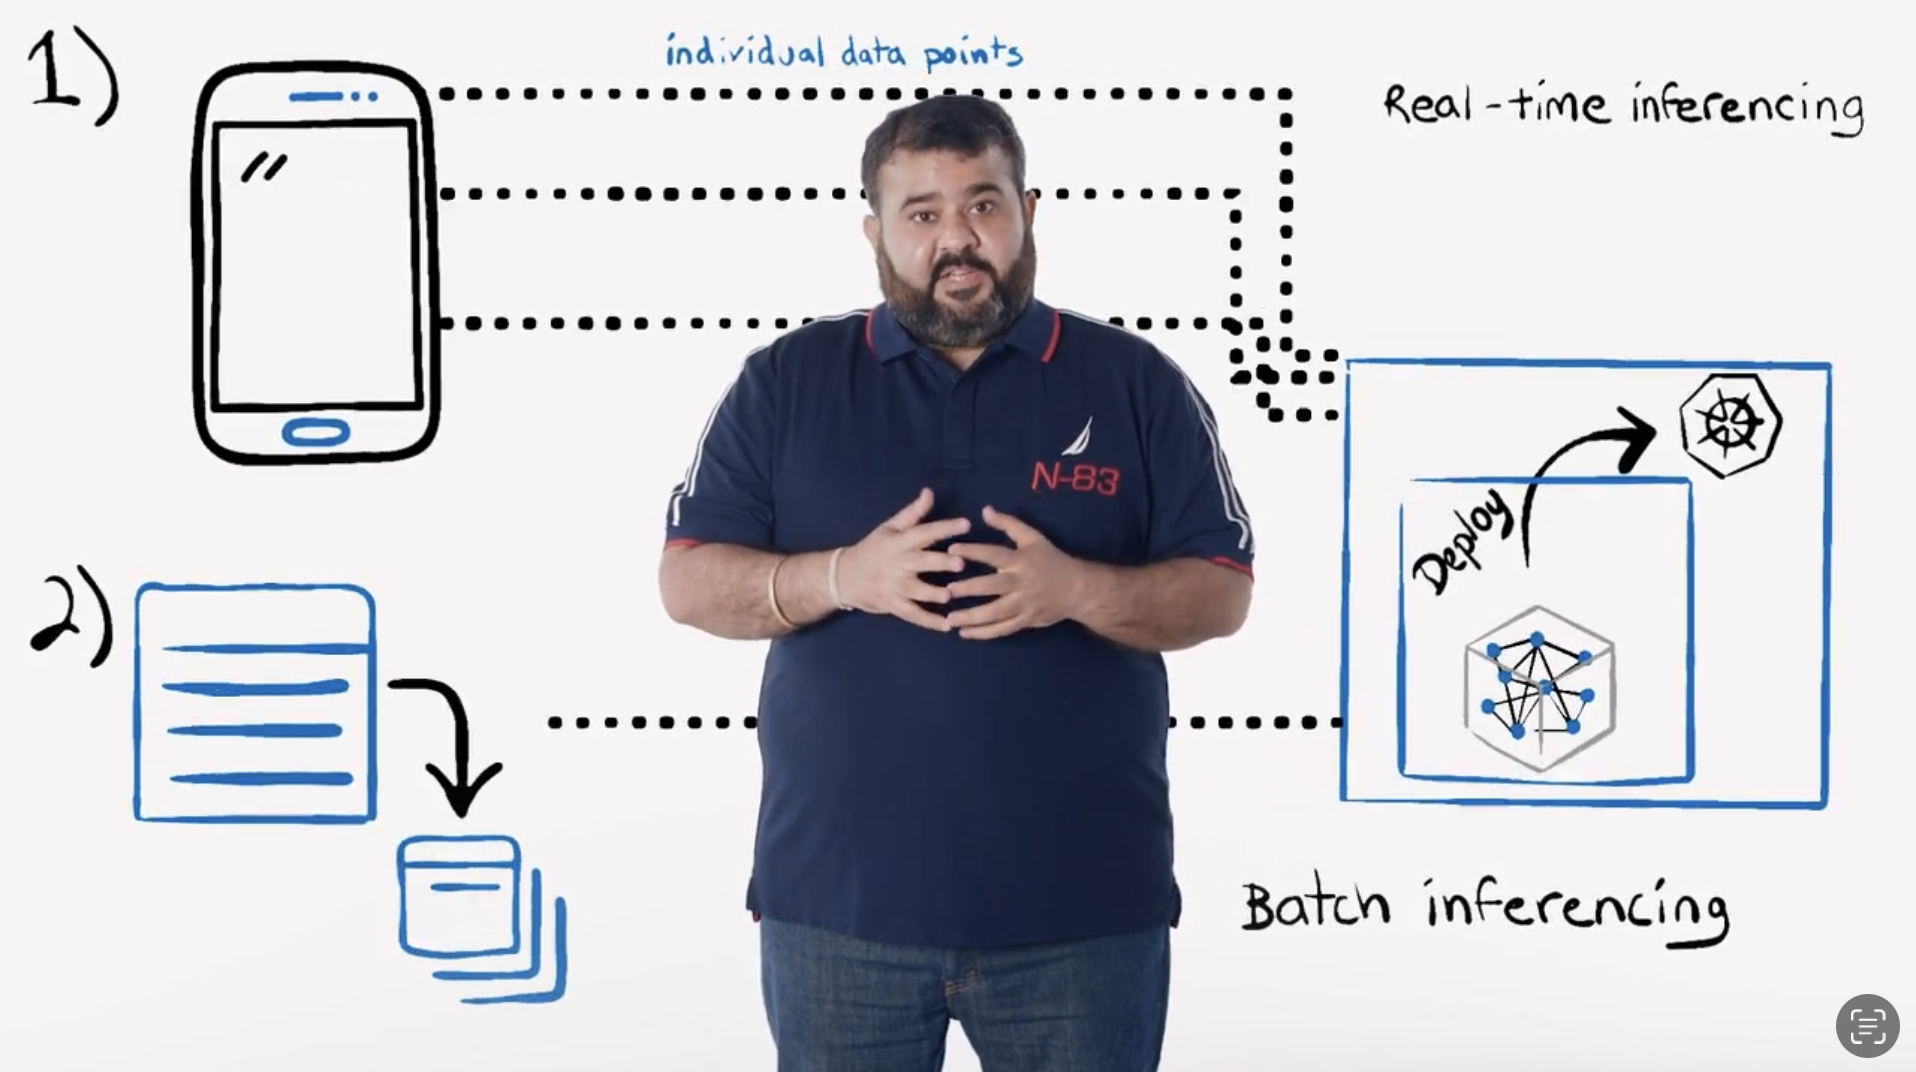
\includegraphics[scale = 0.1]{attachment/chapter_10/Scc012}
	\caption{Inference modes - Two ways of making a inference call}
\end{figure}

In the first option a tupel $(...)$ is send to the model, which sends back the evaluated tupel. This is mostly done, when low latency is required for example
\begin{itemize}
	\item predicated maintance
	\item real-time personalisation.
\end{itemize}
On the other end a decision is needed.\\

The later option transfers or sends a point to a batch of data which the model should be evaluating. Uses cases can be Sales Forcast.

\subsection{Deployment Topologies}
\paragraph{Three Base Container Image Components}
For the deployment of a model three components need to be given, to make a successful inference call.
\begin{itemize}
	\item Environment, which encapultes all the dependencies for a model (requirments)
	\item Scoring code, which specifies who the model is called and the evaluation takes place
	\item inference configuration, takes care of all other components, which is required to call the model 
\end{itemize}

\begin{figure}[H]
	\centering
	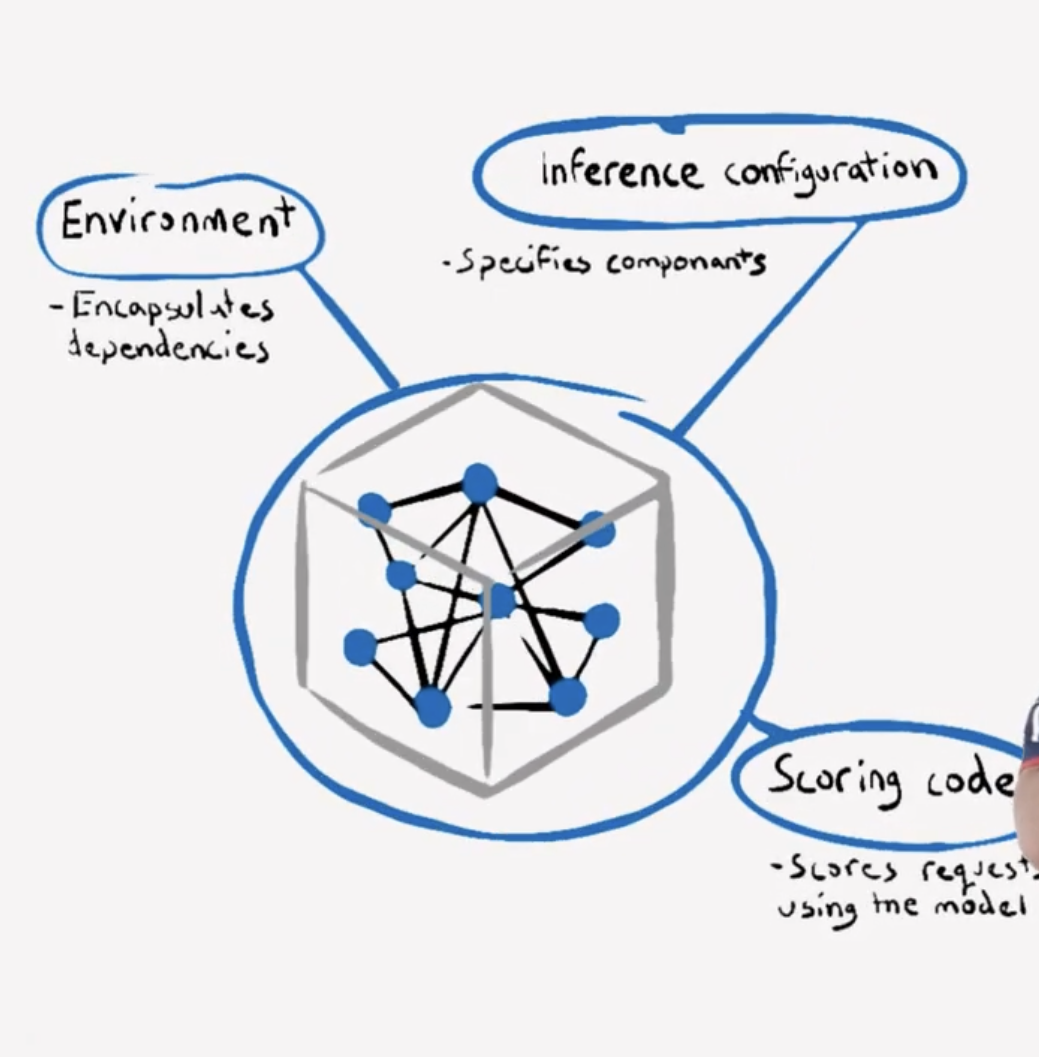
\includegraphics[scale = 0.2]{attachment/chapter_10/Scc013}
	\caption{Deployment Topologies - Environment Component}
\end{figure}

\paragraph{Three topologies}
The previous discusses three components are placed in a \textit{Base Container Image}, which becomes the \textit{Execution Environment} for the model. 

\begin{figure}[H]
	\centering
	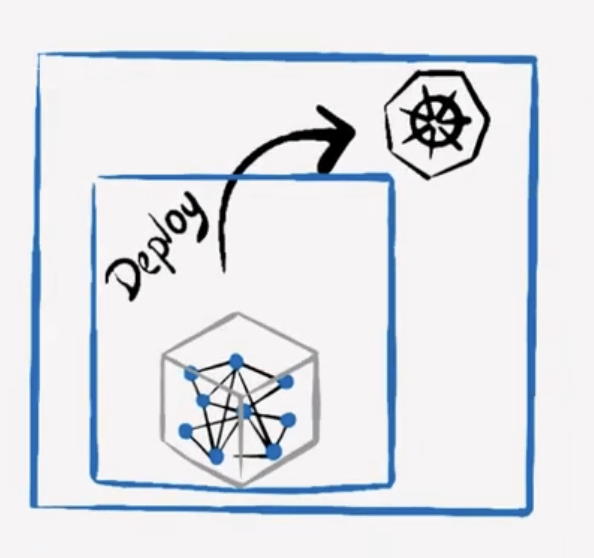
\includegraphics[scale = 0.3]{attachment/chapter_10/Scc014}
	\caption{Deployment Topologies - Base Container Image -> Execution env. for the model}
\end{figure}

This container image has a \textit{load balanced} \textbf{\gls{HTTP}} \textit{Endpoint}, which receives data to be scored. This process of \textit{setting up the Base Container Image/ Execution Environment} can happen in three different ways.
\begin{description}
	\item[No-code-deployment] In the no-code deployment is done by Azure ML in a simple way, in which the model with all it's dependency is deployed into the automatic created container. This is done mostly when using \textit{Designer} or \textit{Auto-ML} capabilities.
	\item[System Image] This is done, when using code-options like \textit{VSCode} or \textit{Jupter Notebooks} through \textit{Azure SDK}.  In give you more flexiblity in configuring the base container, when automatically creating the system image. In this case also the the latest dependency are already installed, like \gls{g_conda} packages.
	\item[\gls{BYOC}] This option let's you create you own container, with allows you to configure it the most.
\end{description}

\begin{figure}[H]
	\centering
	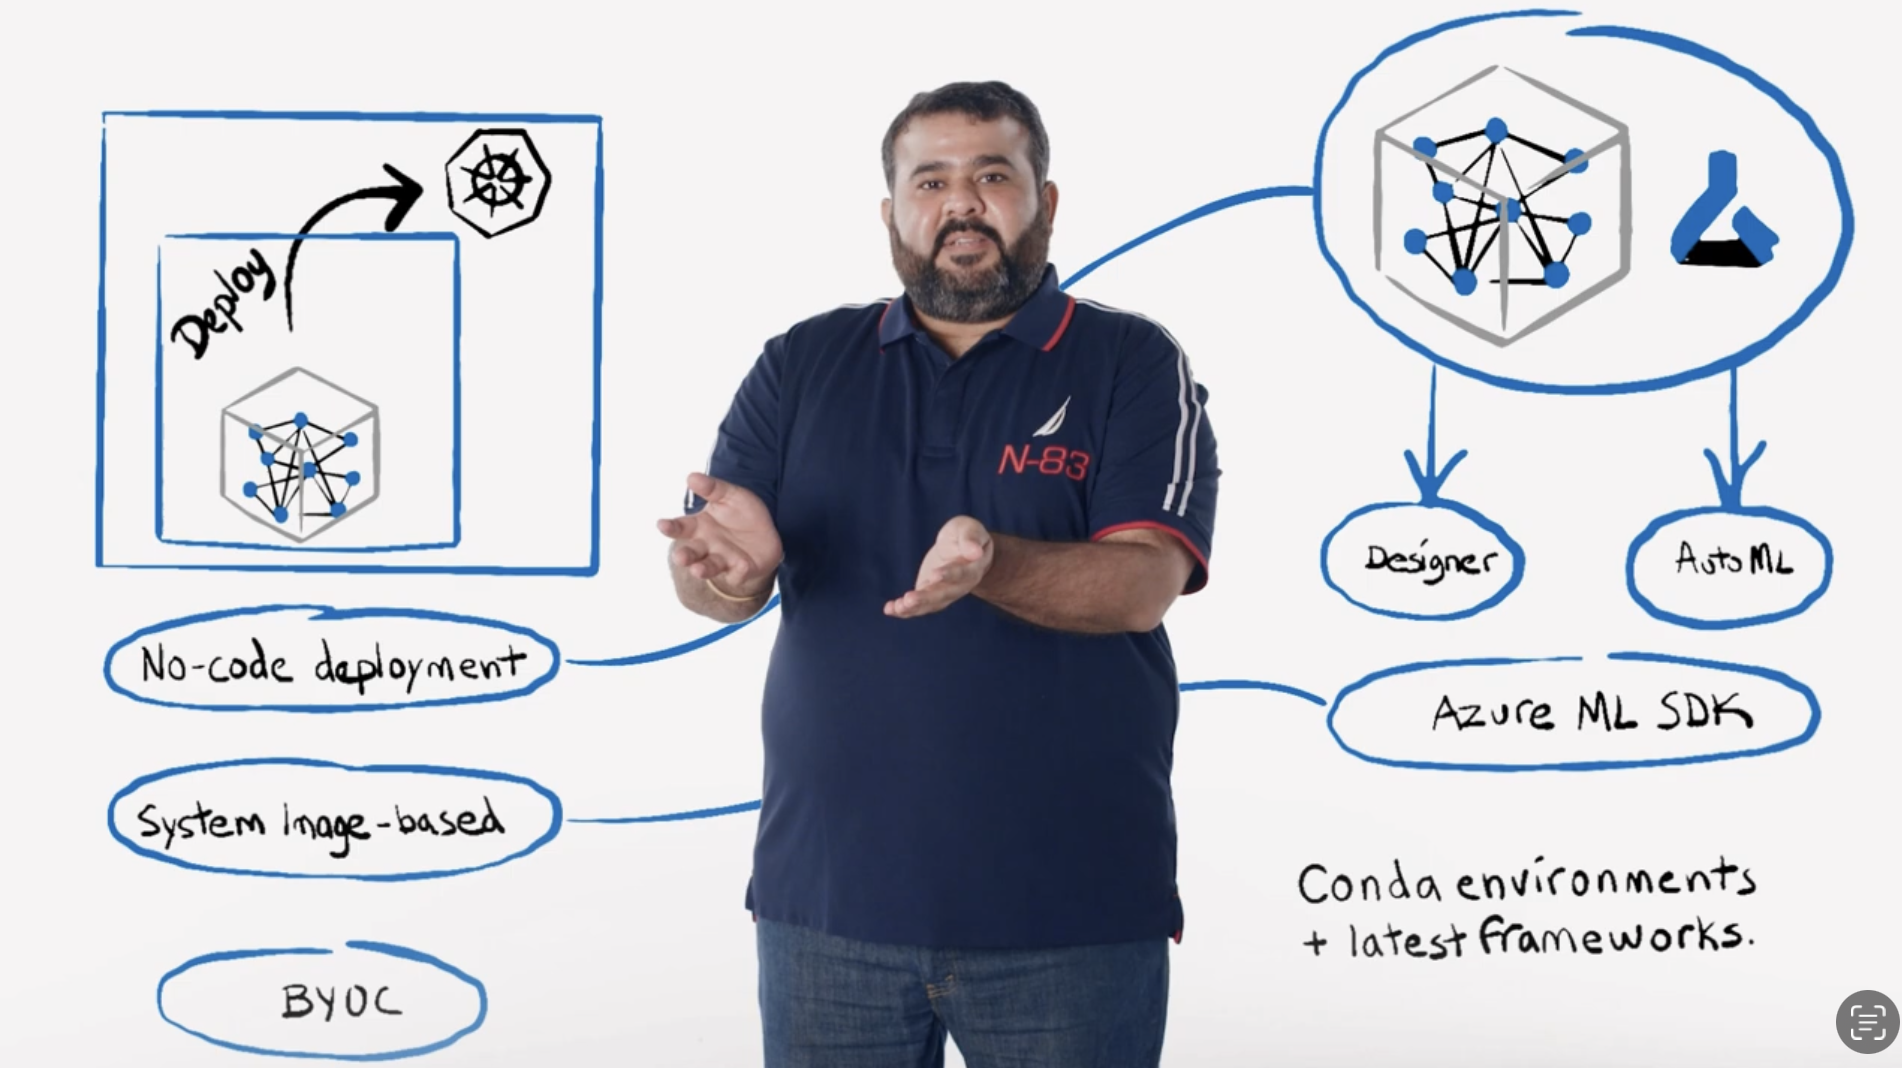
\includegraphics[scale = 0.2]{attachment/chapter_10/Scc015}
	\caption{Deployment Topologies - Three Options}
\end{figure}


The next question is, what resources are needed. 
\paragraph{Self-manage endpoints}

The first two options are for testing the deployment of the containers. The are having a low compute power (*only applies to \gls{ACI}). The later once are for a production requirments.

\begin{figure}[H]
	\centering	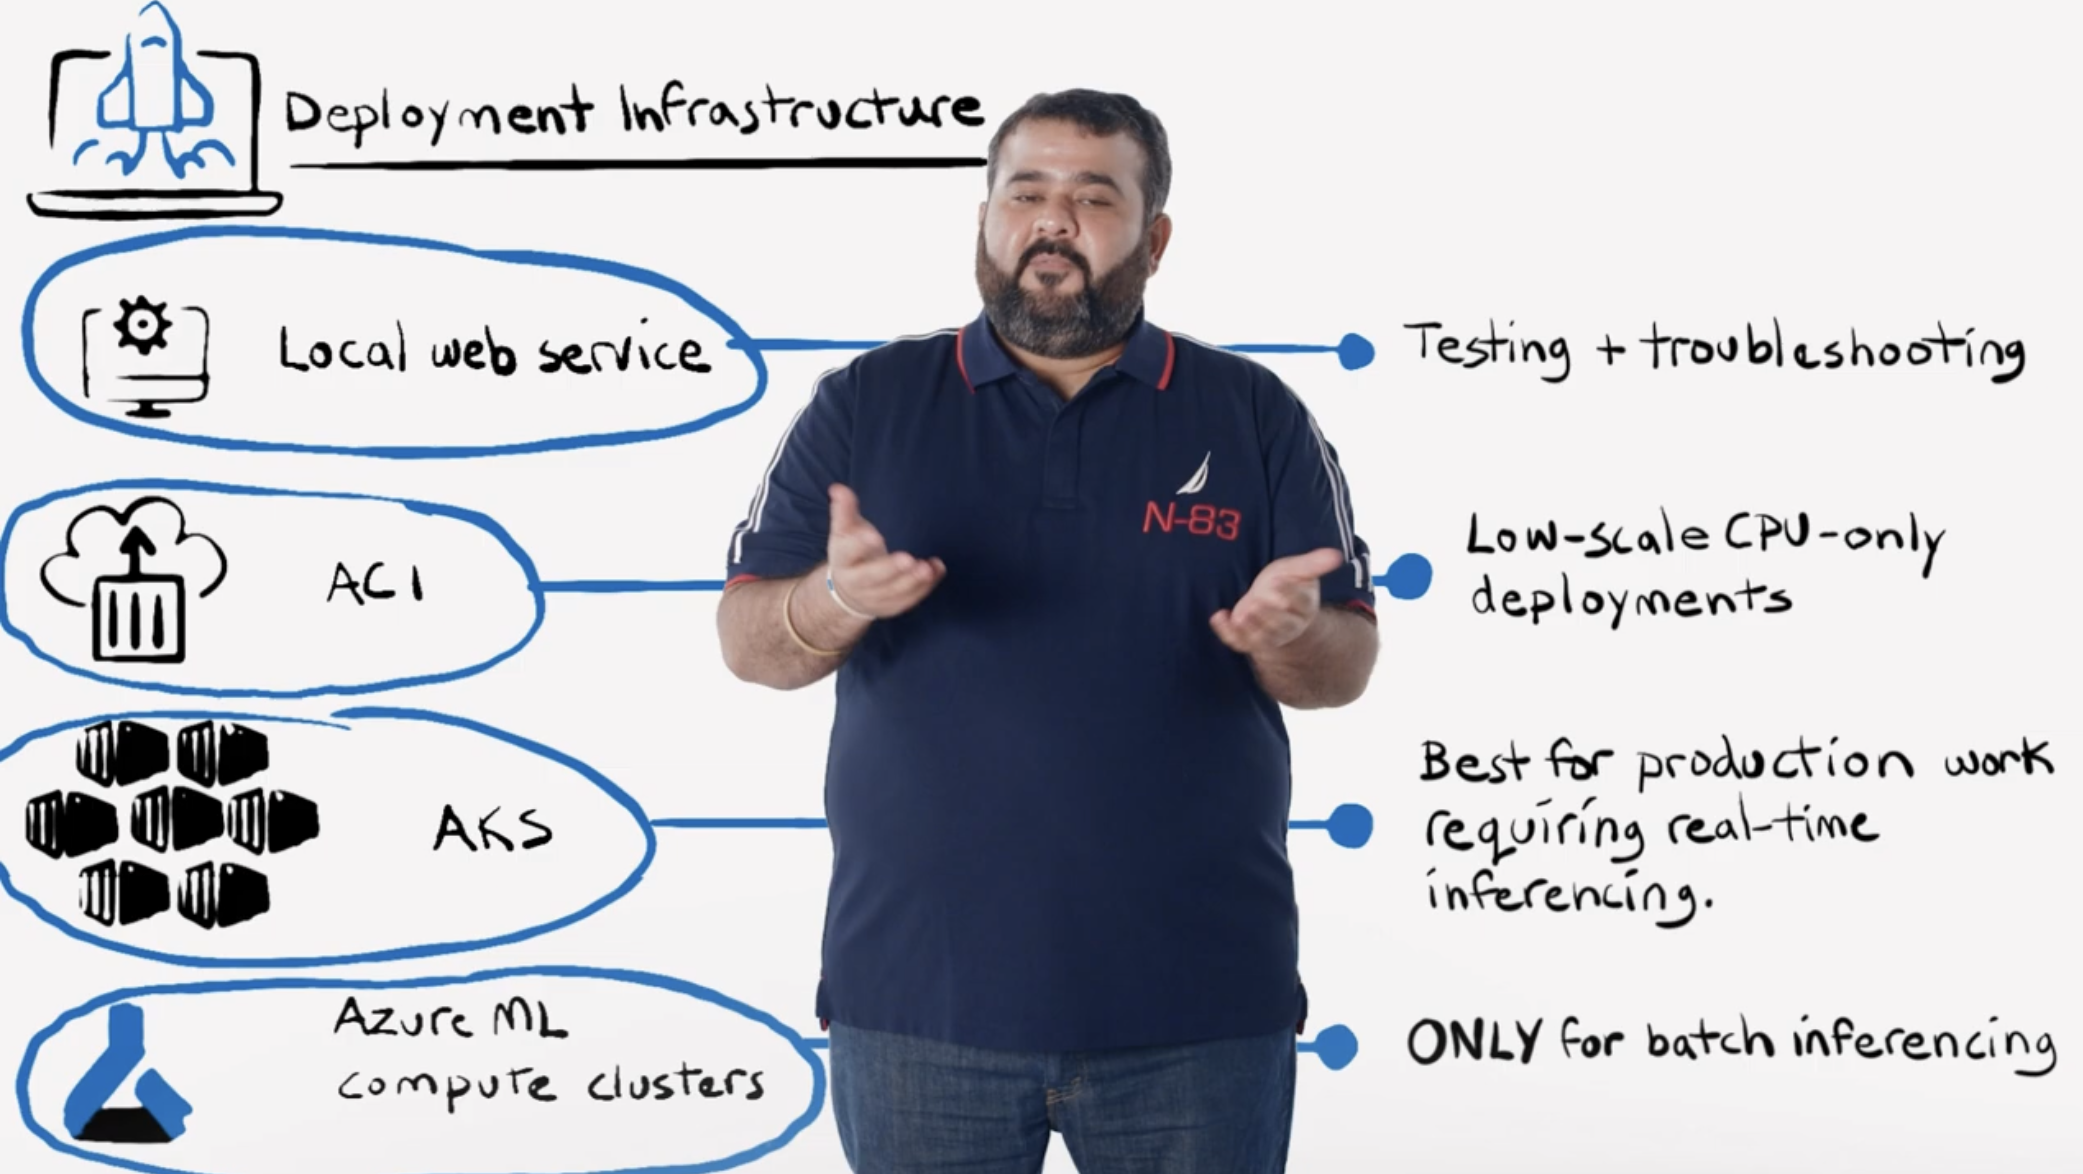
\includegraphics[scale = 0.2]{attachment/chapter_10/Scc016}
\caption{Deployment Infracstrucre - Compute Power Options}
\end{figure}
	

\begin{description}
	\item[Local web service/ \gls{ACI}] This option is for testing and trouble shooting the deployment/ conecting of the container, with the model image to the $"$live$"$ mode.
	\item[\gls{AKS}] This service is needed for production workload for either realtime or batch inferencing. This option can scale up, as the workload increases.
	\item[Azure Compute Clusters] This service is also used for the model training. This compute resources is set up for batch inferencing.
\end{description}

The production service \textit{AKS} and \textit{Azure Compute Cluster} comes with Monitoring and authentication capabilities. 

\paragraph{Managed endpoints}
A new Option takes a way any admistration of the compute cluster. This endpoints is design to allow 
\begin{itemize}
	\item managed online endpoints (Real-Time Inference)
	\item and managed batch endpoints (Batch Inference)
\end{itemize}

\begin{figure}[H]
	\centering	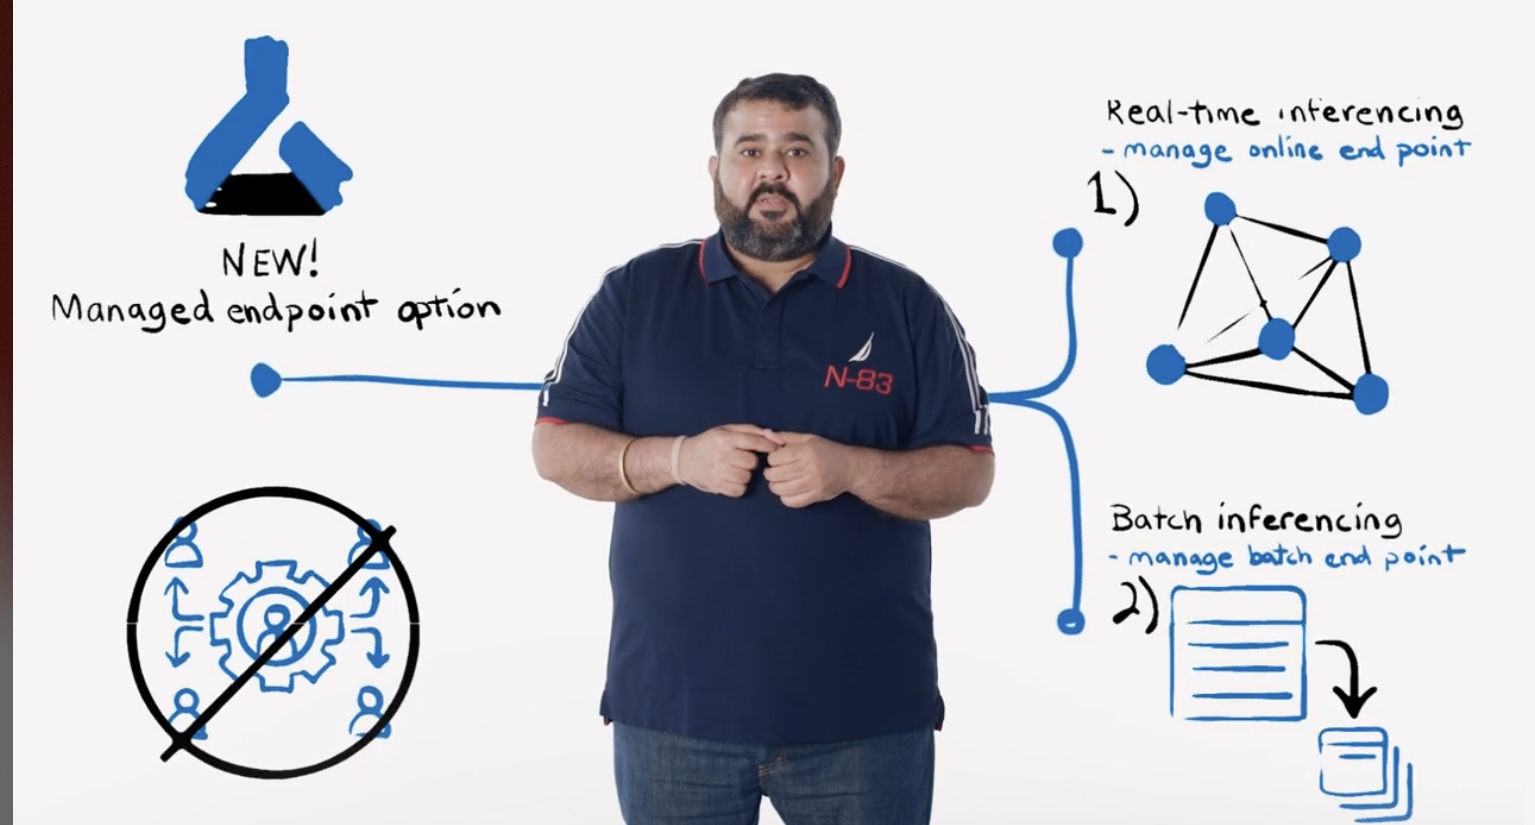
\includegraphics[scale = 0.2]{attachment/chapter_10/Scc017}
\caption{Managed Endpoints}
\end{figure}

For a managed endpoint the 
\begin{itemize}
	\item model 
	\item model version
	\item and compute instance
\end{itemize}

is provied in form of a \gls{.yaml} file.

\subsection{Inference Optimization options}

\paragraph{ONNX}
Many \gls{ML} Model Frames support the convertion of its model to \gls{ONNX}. This is a open standard for representing \gls{ML} models. A inference call to a \gls{ONNX} model can be optimize by using \gls{ONNX} Runntime. This Runner is there to accelerate the hardware components.

\begin{figure}[H]
	\centering	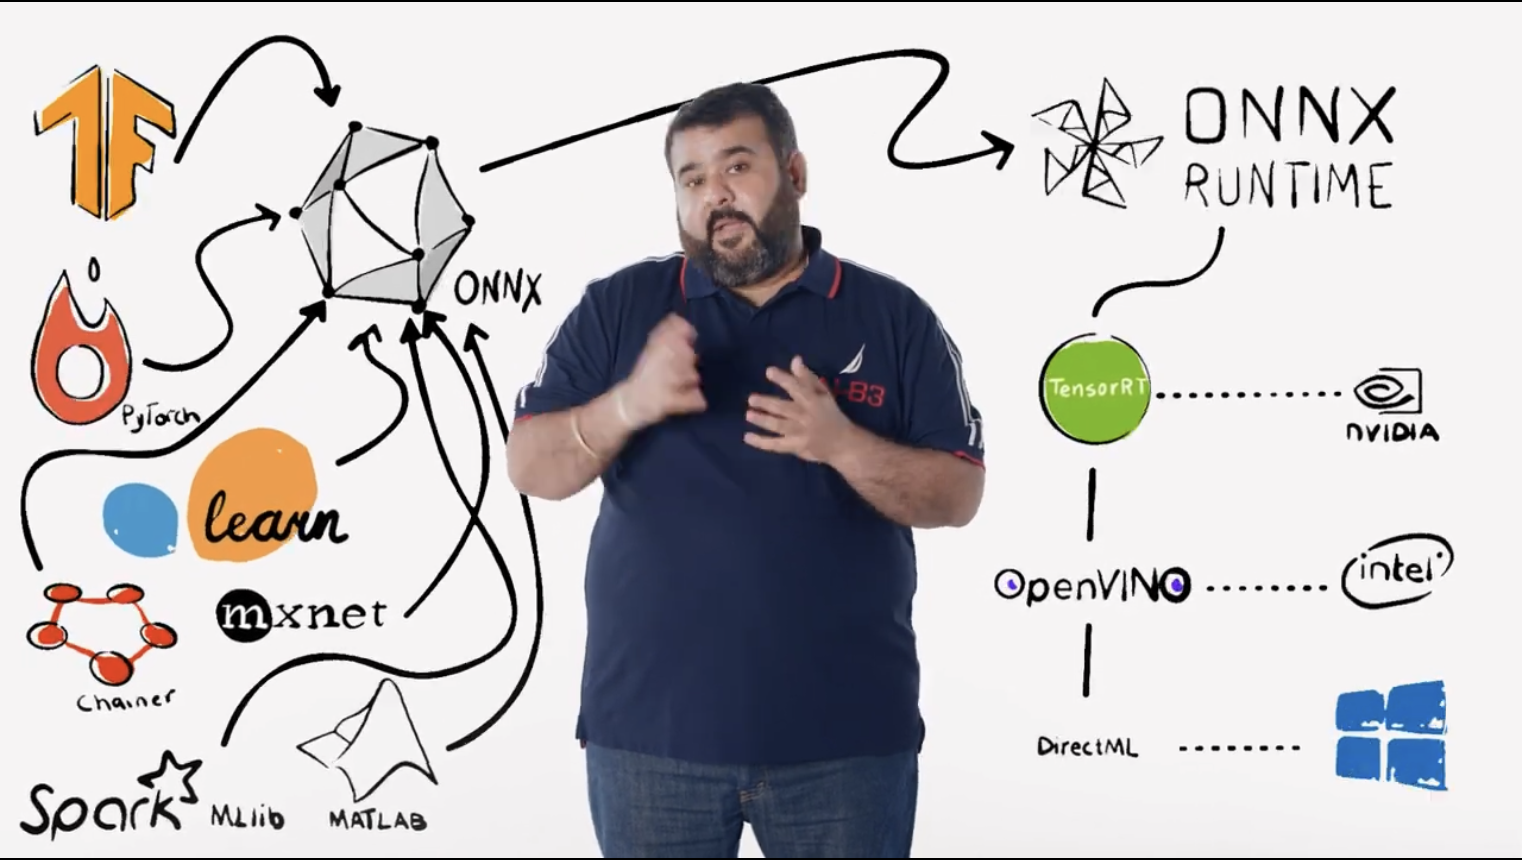
\includegraphics[scale = 0.2]{attachment/chapter_10/Scc018}
\caption{\gls{ONNX} ecosystem}
\end{figure}

Die Optimierung auf verschiedenen Platformen ist am besten erreicht, wenn ein Standardformat für die Modellierung verwendet wird.

\paragraph{Trition}
Trition seems to be a optimization for serves, in order to use \glspl{GPU} and \glspl{CPU} better. On top can be used \gls{ONNX} runtime.

\begin{figure}[H]
	\centering
	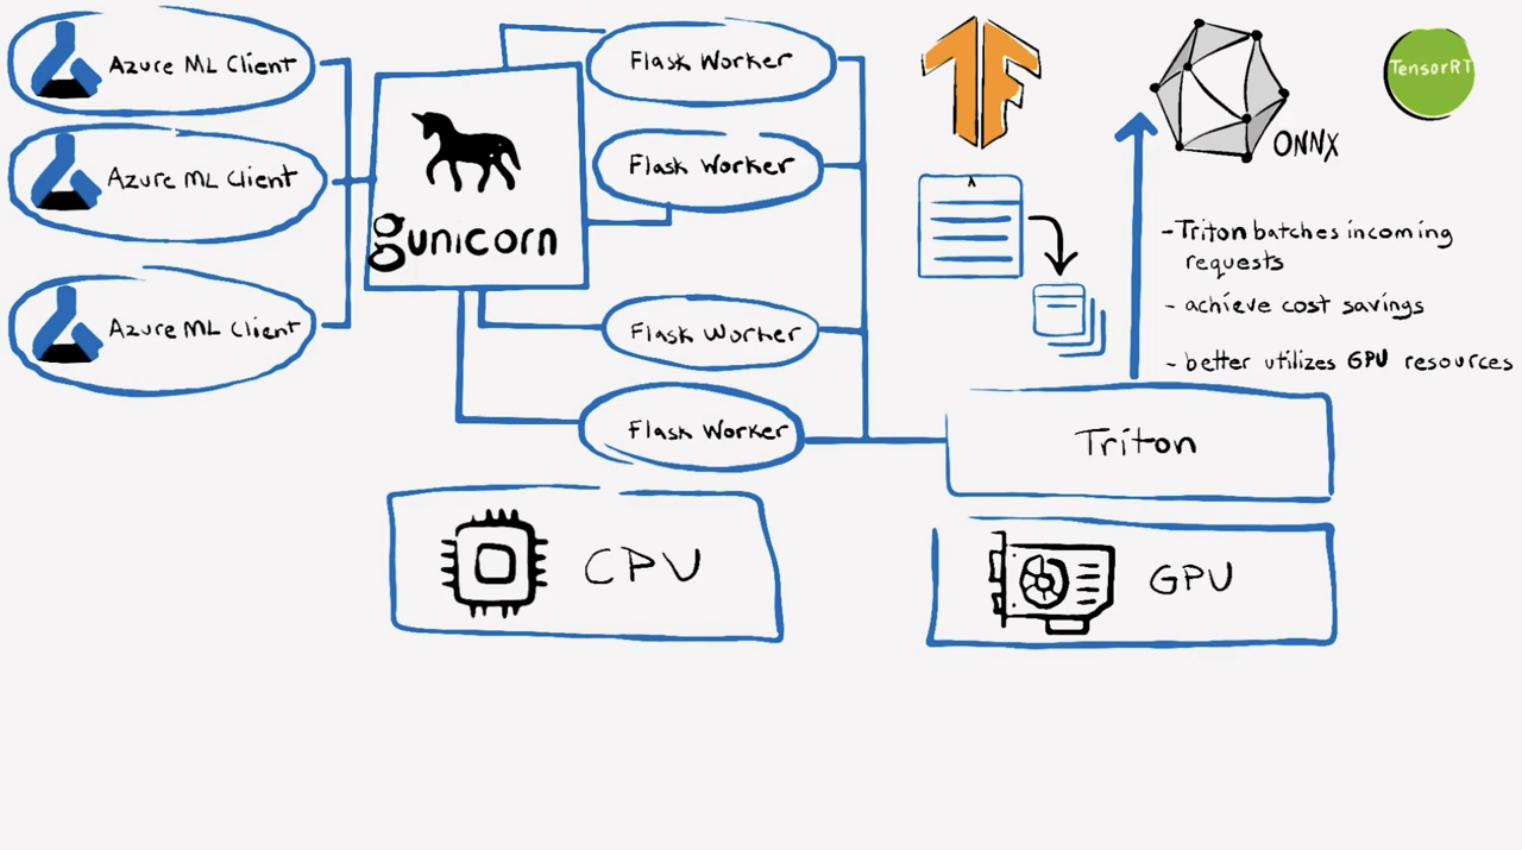
\includegraphics[scale = 0.2]{attachment/chapter_10/Scc019}
	\caption{Trition Optimization}
\end{figure}
This option is important for high frequency real time inferenes.


